\documentclass[titlepage]{article}
\usepackage{setspace}
\usepackage{subfigure}
\usepackage{titlesec}
\usepackage{mdframed}
\usepackage{listings}
\usepackage{tikz}

\setcounter{secnumdepth}{4}

\lstset{frame=tb}

\pagestyle{plain}
\usepackage{amssymb,graphicx,color}
\usepackage{amsfonts}
\usepackage{latexsym}
\usepackage{a4wide}
\usepackage{amsmath}

\newtheorem{theorem}{THEOREM}
\newtheorem{lemma}[theorem]{LEMMA}
\newtheorem{corollary}[theorem]{COROLLARY}
\newtheorem{proposition}[theorem]{PROPOSITION}
\newtheorem{remark}[theorem]{REMARK}
\newtheorem{definition}[theorem]{DEFINITION}
\newtheorem{fact}[theorem]{FACT}

\newtheorem{problem}[theorem]{PROBLEM}
\newtheorem{exercise}[theorem]{EXERCISE}
\def \set#1{\{#1\} }

\newenvironment{proof}{
PROOF:
\begin{quotation}}{
$\Box$ \end{quotation}}



\newcommand{\nats}{\mbox{\( \mathbb N \)}}
\newcommand{\rat}{\mbox{\(\mathbb Q\)}}
\newcommand{\rats}{\mbox{\(\mathbb Q\)}}
\newcommand{\reals}{\mbox{\(\mathbb R\)}}
\newcommand{\ints}{\mbox{\(\mathbb Z\)}}

%%%%%%%%%%%%%%%%%%%%%%%%%%


\title{{\vspace{-14em} 
\includegraphics[scale=0.4]{ucl_logo.png}}\\
{{\Huge Impact of automatically generated tests on the genetic improvement process}}\\

}
\date{Submission date: 5 May 2020}

\author{Lim Mingyi\thanks{
{\bf Disclaimer:}
This report is submitted as part requirement for the BSc Computer Science programme at UCL. It is
substantially the result of my own work except where explicitly indicated in the text. The report may be freely copied and distributed provided the source is explicitly acknowledged.}

\\ \\

BSc Computer Science\\ \\
Dr Justyna Petke}

\begin{document}
 
\onehalfspacing
\maketitle

\vfill
\pagebreak

\begin{abstract}
Genetic improvement (GI) uses automated search to improve existing software. GI can be used to improve runtime, energy consumption, fix bugs and more. GI usually relies on testing to validate the evolved program changes. The aim of this project is to establish what characteristics the test suites should have in order to improve the effectiveness of the GI process. In this study, we automatically generated test suites with EvoSuite using different criteria, and used them as input to GI to assess their impact on the patches generated. We find that while test suite coverage has an impact on the ability of GI to produce correct patches which do not overfit, it did not have an impact on the runtime improvements found by the patches. We also compared automated tests to manual, developer written tests and found that while manual tests were more likely to produce patches which maintained a program’s core functionality, automated tests were more likely to find better improvements when used as input to a GI process.

\end{abstract}
\vfill
\pagebreak

\tableofcontents
\setcounter{page}{1}
\pagebreak

\section{Introduction}
Software engineers and programmers constantly seek ways to improve the properties of their code. From correcting bugs in software, to improving the non-functional properties of software such as runtime, memory usage or even power usage of a program, these tasks require efforts from skilled software engineers to generate working solutions. In this study, we build upon prior research on the feasibility of using search-based software engineering techniques to solve these software engineering problems faced by developers and engineers.


Genetic Improvement is a relatively new area of knowledge that aims to generate improvements to existing software through iterating through the search space of candidate patches and applying them to an existing program to find functional or non-functional improvements to existing software \cite{petkesurvey}. A subset of GI is that of Generate and Validate (G\&V) methods, where candidate patches are generated and evaluated against a test-suite and some fitness functions \cite{harman2012,harman2007}. In GI, patches are generated iteratively using a sequence of mutations to the original code. Mutations are defined as edits made to the program at source code, assembly or binary level which involve operations such as deletions, replacement or insertion of code at either the statement or line level, though other mutations have been used \cite{petkesurvey}. Mutations are then assessed by a fitness function which provides a measure of how good a program variant is based on the goal of the process. Mutations which improve the score on the fitness function and pass all test cases in the provided test-suite are seen as improvements, kept, and are further mutated. Through this process, we are able to narrow the search space of candidate patches and find those which improve properties of the software.

Previous research on genetic improvement techniques for non-functional improvement (NFI) has shown promise. In a previous experiment conducted by Bruce et al \cite{bruceenergy}, GI was shown to be able to reduce the power consumption of programs by 2.7\% on average. Langdon and Harman were able to achieve significant performance advantages in software\cite{langdonharman2015}, and Wu et al was able to use GI to reduce memory use \cite{yuewu2015}. These results provide the motivation for future work in the future on NFI using genetic improvement.\\

In this process, the test suite plays an important role in determining the success of the patches \cite{qireiss2017}.  Given that we evaluate candidate patches during the genetic improvement process by their ability to pass the provided test suite, the test suite serves to guide the process of genetic improvement. A poorly formed test suite which fails to encapsulate the required behaviour of the program might still pass when the mutated program breaks some key functionality. Conversely, a test suite which places unnecessary restrictions on program behaviour might prevent the program from improving as much as it might be able to. Identifying the optimal properties of test suites used as inputs to the Genetic Improvement process is thus crucial to the success of generating strong, correct patches. 

The prospect of using automatically generated test suites as input to the GI process can potentially provide a simple way of generating improvements for programs quickly. Since automated test suites can be easily generated from just the source code, they can be generated at scale, and much more quickly than user written tests. Using automated test suites in conjunction with genetic improvement techniques, we can potentially automate the entire process of genetic improvement for non functional improvement, removing the need for user supervision or input. However, there is currently little research around the use of automatically generated test suites as input to the GI process.

Previous work on the use of automated tests in GI focuses mainly on improving functional properties of software. This application of GI precludes the use of automated testing as an input to the process because functional improvement relies on the existence of an oracle apart from the program to specify the correct behaviour of the program. However, in the case of non-functional improvement of the program, we assume the original source code to already fulfil all functional requirements of the program. Since it is already correct, the original source code can be used as an oracle which describes the functional requirements of the program. \cite{petkegin} As such, we can theoretically use automated test generation tools to create a test suite which captures the current behaviour of the program, and thus use this generated test suite as an oracle to guide the GI process. The use of automated testing here should thus be feasible and beneficial as it could be a suitable replacement for manual test suites where they don’t exist, or to augment the manual test suites in cases where they are not strong enough.
Building on previous work, our research thus aims to assess the feasibility of using automatically generated test-suites as input to a genetic improvement process, as well as to investigate the attributes automated test-suites should have to produce optimal results in the improvement of non-functional attributes of programs. This can guide us in understanding how automatically generated test suites might possibly work as inputs to the GI process, as well as develop a sense of which test suite characteristics contribute most to the success of a test suite in generating good patches.

All data and scripts used in this experiment are made available at : https://github.com/mingyi850/gin so the results obtained in this experiment can be replicated.


\section{Background}
Current literature around automated program repair and GI is mostly centred around automated program repair using Genetic programming \cite{petkesurvey}. However, common threads between the 2 fields exist which could be useful for our work on non-functional improvement of software.

\subsection{Genetic Improvement}
Genetic improvement uses automated search to find improvements to existing software\cite{petkesurvey}. Born out of ideas to automate the software engineering process, genetic improvement in software traverses the search space of available software, guided by some search algorithms such as metaheuristics, to find variants of the original source code which constitute improvements to the original software. In the context of non-functional improvement, such a variant preserves all its original functionality while offering evident improvements in some property unrelated to its function.

Recent advances in the availability of large amounts of source code has allowed the field of genetic improvement to make big strides, while popularising genetic programming, or mutation from an original source over program synthesis, which aims to construct programs from scratch. \cite{petkesurvey}. The large amount of source code available provides a large reservoir of genetic material which can be used in the GI process. 

These techniques have proven to be relatively successful in performing a variety of tasks from program repair to non-functional improvement.
Literature around genetic improvement (GI) has heavily focused on program repair. This is an application of GI that aims to modify some functional properties of the programs, via guidance from a test suite. These experiments have been largely successful \cite{cure,genprog} and have shown GI’s ability to improve some functional properties of programs.

\subsubsection{Overview of a GI Process}

The genetic improvement process uses automated search to find improvements in software by traversing the search space of available variants of the program. Typically, it takes in a program which is to be improved and a test suite as input. The program is first represented in a form which the GI process can work with, such as an abstract search tree (AST),or BNF like grammar \cite{langdonharman2015}. It then makes modifications to the program at the source code or binary level using a suite of mutation operators such as deletion, insertion, and replacement of statements at a level of granularity specified by the algorithm used. 

The GI process uses a genetic programming which mimics evolution in living organisms by working in ‘generations’, where several variants of the original program are spawned. Each of these initial variants contain a single mutation and is known as the initial population. From this initial population, the GI process applies mutations to each of these initial program variants for a set number of generations  \cite{petkespecialise}. With each generation, the new program mutants are evaluated by a user-defined fitness-function, which provides some measure of how desirable the mutant is. This fitness-function is typically a function of the program's functional aspects (ability to carry out a task correctly) as well as non-functional properties such as memory usage and runtime, but can be extended to include any measurable aspect of the program \cite{fitnessfunction}. At various points in the process, mutants which do not meet a specified threshold in fitness are killed. This is known as selection. Remaining mutants can continue the mutation process, either through the application of more mutation operators or via a combination of existing mutations found in the current generation. 
The GI process continues for a specified number of generations, looking for improved variants of the source code. Once it is completed, the process selects the mutant with the highest fitness score. The patch applied to the original program to achieve this mutant is considered the best patch and is returned by the GI process.

\subsection{Overfitting}

Overfitting is a phenomenon which occurs when a patch generated during the genetic-improvement process passes all the test cases of the supplied test suite used to evaluate its fitness but breaks existing functionality or fails to behave as it should on untested functionality. It occurs as test suites are imperfect representations of a program’s correctness \cite{cure}. This is a problem in G\&V methods as the process relies on the input test-suite as an oracle for program correctness. Patches which fail to exhibit correct behaviour can undermine the performance improvements found through the process. Smith et al \cite{cure} show that test-suite coverage and overfitting in program repair are highly correlated, and that automated test-suites tend to exhibit higher rates of overfitting in patches for functional improvements due to the lack of diversity of generated test suites. Subsequently, Qi and Reiss \cite{qireiss2017} have identified means to identify and thus filter out these overfitting patches through augmentation of the original test suite with additional generated tests . While much of the above research has been done on program repair, which aims to fix some failing test suite, in Non-functional Improvement, the input program can be used as its own functional oracle \cite{petkegin}. However, poorly generated test-suites can still lead to overfitting, if the test-suite does not encapsulate all functional behaviours of the program. As such, overfitting and maintaining the functional properties of generated patches are still an area of concern in Genetic Improvement. Recent studies \cite{cure,yicorrelation} point to the use of more diverse and robust test suites to reduce the risk of overfitting.


\subsection{Related Work}

A large amount of research has gone into trying to solve the overfitting problem in program repair. Qi et al \cite{qireiss2017} describes a method to validate the correctness of generated patches through additional test cases, while Xiong, Liu et al \cite{xiongliu2018} use a distance-based approach to assess the correctness of a test and its patches. Both methods provide further methods of validation to reduce or remove overfitting in program repair. In the context of Non-functional improvement however, the use of additional test cases might be more apt.

While studies have been conducted on Genetic Improvement techniques, there has not been one which shows the relationship between non-functional improvement and automated testing.

A study conducted by Yi, J, Tan et al \cite{yicorrelation} aimed to find the correlations between different conventional and non-conventional test-suite metrics and the reliability of generated patches. It measured the relationship between branch coverage, statement coverage and test-suite size against the regression ratio which identifies unreliable tests. They showed that while all 3 attributes were strongly negatively correlated with regression ratio, statement coverage was the most highly correlated at r=-0.92 . This suggests that statement coverage can be targeted as the most important metric in our automatically generated tests to ensure reliability in program repair.
Yu, Martinez et al \cite{yumartinez2019} further find methods to solve the overfitting problem by augmenting user provided test-suites with automatically generated test-suites to further constrain the patches produced. However, their results are limited to synthesis-based software repair which aims to construct programs from scratch through guidance from a specification.

On non-functional improvement, Bruce et al’s \cite{bruceenergy} work on improving energy consumption of programs through GI shows promising results, but their solution evolves solutions which pass only an appropriate number of tests rather than all tests. While they managed to succeed in reducing energy consumption in this study, automatically generated test-suites were not used to guide the GI process.

Genetic Improvement has also been applied to large-scale software systems to improve efficiency and memory usage of software \cite{yuewu2015}. However, like in Petke et al's study on improving energy consumption \cite{bruceenergy}, the test cases here were human-developed and robust. Which means that overfitting is less of an issue. This sentiment is echoed in \cite{cure} where automatically generated test-suites resulted in more overfitting than manually, professionally written ones in program repair.  That being said, we cannot always rely on the existence of an effective test suite for a program. Automated testing provides a consistent option for software testing, which can be used in the absence of a manual test suite or where a manually written test suite is not effective on it's own.

The space automated test generation for Non-functional improvement in Genetic Improvement is one which has not been explored fully. However, by drawing on previous work on Genetic Improvement, Program repair, and current work on Non-Functional improvement in Genetic improvement, we can develop some intuition and conjectures on the problems and solutions which will drive our research. 


\section{Project Aims}

Current research around GI is currently focused on program repair rather than non-functional improvement. \cite{petkesurvey} Furthermore, studies on GI for non-functional improvement do not take into consideration the challenges around the use of automated test-suites in the GI process. Previous studies on GI for NFI do not take overfitting into account as the program itself is assumed to be already correct and the test suites provided in those studies were typically developer-written and robust\cite{petkegin}. While in program repair, developer written test suites are relied upon to specify the required behaviour of the program, automated test suites can be used in non-functional improvement as the test generation process can presumably leverage and thus capture the behaviour of the existing, correct program. However, automated test suites lack the same intuition that developers do. While coverage based methods of test suite generation are focused on achieving high coverage of software, they are ultimately unable to understand the software at a higher level. This results in the inability of automated test suites in reliably capture a program's intended behaviour \cite{evosuitefaults} also evidenced by the generation of ‘flaky’ assertions \cite{coveragecombination}. As shown by Qi and Reiss \cite{qireiss2017}, the use of test suites which do not correctly encapsulate the behaviour of the program in the GI process can lead to overfitting. This then leads us to the questions - how can we ensure that we reduce the impacts of overfitting when using automated test suites as inputs to the GI process? What characteristics should automatically generated test suites possess to maximise improvements in the GI process, while minimising overfitting?

With these questions in mind, this paper seeks to fill in the knowledge gap around the use of automated test suites in Genetic Improvement. To do so, we conduct a study on 4 test suite generation criteria, the coverage metrics they aim to optimise, and their impact on the patches generated though GI process. We evaluate these test suite criteria and their corresponding coverage metrics on their ability to
\begin{enumerate}
	\item Produce patches which do not overfit to the test suite provided, and 
	\item Produce patches which provide the highest reduction in runtime of a program. 
\end{enumerate}	
Ultimately, we seek to answer the following research questions:
\bigskip

\begin{mdframed}
	\textbf{
	Research Question 1: How do test generation criteria and coverage metrics in automated tests 
	affect overfitting in patches generated through the GI process?
	}
\end{mdframed}


Given the range of issues around the use of automated testing in the GI process, we want to first identify key traits of automated test suites which can lead to lower rates of overfitting in patches generated. This will provide us an intuition for understanding the relationship between these characteristics and overfitting in the resultant patches.\\

\begin{mdframed}
	\textbf{
	Research Question 2: How do test generation criteria and coverage metrics in automated tests 			affect performance improvements gained by patches generated through the GI process?
	}
\end{mdframed}

The ability of a patch to provide increases in performance of software is ultimately the main aim of non-functional improvement. As such, we want to assess the efficacy of automatically generated test suites as input to the GI process, as well as to find out which characteristics of test suites can lead to the largest gains in performance of software.\\

\begin{mdframed}
	\textbf{
	Research Question 3: How do automated test suites compare to manually written test suites in 			terms of generating patches which do not overfit and creating performance improvements in the 			source code? 
	}
\end{mdframed}

Lastly, we want to measure how well automated test suites perform against manually written test suites as input to the GI process. In this section we compare the results obtained from the use of automatic test suites and manual test suites on both overfitting and the performance improvements gained.  This will allow us to find if there are more advantages in using automatically generated test suites as input to the GI process. 


\section{Dataset and Tools}


\subsection{Gin}
In this study, we built our experiment around Gin, an extensible and modifiable genetic improvement tool developed by David R. White, and later expanded by Brown et al. \cite{petkegin}. Gin uses search-based software engineering techniques to find suitable patches and optimisations for Java programs. It focuses on non-functional improvement (NFI) of programs, using a supplied test suite as an oracle to ensure the correctness of the program being optimised. \cite{gincasestudy}

Gin is able to perform edits at either Line or Statement level. At the Line level, source code is represented as a list of lines each one corresponding to a single line of Java code. Modifications to the code are made by making one or more edits to entire lines of code. At the statement level, the source code is  parsed and represented as an Abstract Syntax Tree (AST). This allows Gin to make edits at any level of the tree represented by a node. 
Gin traverses the search-space of possible edits and patches which can be made to a program. It uses operators delete, swap, insert, copy and replace operators to make edits to the source file,, where ‘genetic material’ or code segments for insert and replace are obtained from elsewhere in the source code, based on the ‘Plastic Surgery Hypothesis’\cite{plasticsurgery} by Barr et al, which states that “Changes to a codebase contain snippets that already exist in the codebase at the time of change, and these snippets can be efficiently found and exploited.” This means that the source code contains sufficient material for grafting, and that the material which might lead to a successful patch is likely contained within the same source code \cite{bobbyblind}. 

Gin employs LocalSearch by default as its search algorithm. It starts by applying a random, single-edit patch to the source file. At each step, a random edit is removed or a new randomly generated edit is added to the patch. At each step, the new patch is evaluated. If the patch offers an improvement, the patch is retained and the process is repeated. This continues until the set number of iterations are complete \cite{petkegin}. The final optimal patch is then applied to the source code and saved to a copy of the original source file. 

Our choice to use Gin as the GI framework in this experiment was mainly motivated by several factors. Firstly, Gin is one of only two open-source general GI tools currently available, the other being PyGGI implemented in Python \cite{pyggi2}. While both tools are able to work on Java, Gin is specifically optimised for Java and our experiment specifically targets Java code. Secondly, Gin is the only GI tool that provides a prototype integration with EvoSuite. This allows us to invoke EvoSuite through Gin, automatically generating test suites for our candidate programs using EvoSuite. Gin also allows us great flexibility in modifying and extending its functionality which allows us to create new  classes which will be used for the experiment. In doing so, we are able to design our experimental setup almost completely in Java, using the inbuilt functionality Gin provides. This reduces the need for inter-process communication while also ensuring experimental efficiency. These factors led to our conscious choice to use Gin for this experiment.


\subsection{EvoSuite}
In order to generate automated test suites, we used EvoSuite as a test case generator. Evosuite works using a genetic algorithm to generate test cases for a program. It takes in user inputs to decide on coverage criterion it should optimise, then uses a genetic algorithm to generate test-cases which aim to maximise coverage of the provided source code \cite{evosuitefaults}. EvoSuite continues to produce test-cases until coverage of all user-defined criterion is fully maximised or the end of the prescribed search budget. Once complete, assertions are then produced for each test case to capture the state of the program after each test case. Using this approach, EvoSuite is able to optimise its generated test suites for different coverage metrics, which will be the focus of our study. Due to the large search space of test parameters, we decided to use independent coverage criterion as our independent variable. The variation of coverage goals can also allow us to understand which coverage criteria set at the test generation stage have the greatest effect on the performance of patches produced in the Genetic improvement process.

Using EvoSuite, we were able to set the criterion to optimise for each generated test suite. In this study, we generated tests optimised for 4 different criteria:

\begin{enumerate}
	\item Line Coverage	\\
Line coverage directly measures the percentage of lines the test suite manages to utilize during the process. It tells the user the proportion of lines of code that are executed during the invocation of the test, and is thus a simple way to evaluate the coverage of a test suite. Optimisation for Line Coverage aims to cover as many individual units of the code as possible.
 
	\item Branch Coverage \\
Branch coverage treats the source code as a decision tree, and reports the proportion of conditional branches of this tree tested by the test suite. Optimisation for branch coverage aims to ensure that all conditional branches are reached by the test suite, to accurately capture the spectrum of behaviours of the program. A test suite which has high line coverage but low branch coverage may overlook branches which contain few lines of code in favour of those with a higher number of lines of code. 

	\item Conditional Branch Coverage \\
Conditional Branch coverage \cite{testingtextbook} is a variant of branch coverage which also aims to cover each branch of a test suite. However, instead of simply covering branches, conditional branch coverage ensures that branches are reached with the correct combination of conditions. Take for example the case where we have a function with the following branch:
\begin{lstlisting}
function() {
	IF (cond1 || cond2 || cond3) {
		Outcome a
	}
	ELSE {
		Outcome b
	}
}
\end{lstlisting}
In branch coverage, 2 test cases would suffice in achieving 100\% coverage - one test where cond1 evaluated to True and one where it evaluated to False. With test cases covering both these cases, we can execute all branches in the program and thus achieve 100\% branch coverage of the function. However, one can see that this test only covers a small subset of the expected behaviour of the program - it fails to cover the case where cond2 or cond3 is True  while cond1 is False, or any other combination of cond1, cond2 and cond3 where the if statement would evaluate to True. Optimising for Conditional Branch coverage would require that all these cases are tested for since each condition within the if statement represents a unit to be tested. The same 2 test cases stated above would only achieve a 50\% CBranch coverage, despite covering both branches of the program. Thus, we can see CBranch coverage as a stricter version of branch coverage, which ensures that all conditions are tested.



	\item Weak Mutation \\
Weak mutation \cite{mutation1, mutation2} coverage is a fault based approach to test coverage measurement and is derived from the concept of mutation testing. In mutation testing, a test suite is evaluated by its ability to detect mutations in the source code. In test evaluation, the source code is mutated with one or various edits at the statement level and the test is then run on the source code. The coverage of the test is equal to the proportion of mutants it manages to ‘kill’ or catch. Weak mutation differs from strong mutation in the fact that in Strong mutation, errors due to mutation of a component must propagate to the output of the program, thus requiring a more stringent set of test cases. However, it is stated by Offutt and Lee that Weak Mutation can produce stronger test suites than Strong mutation \cite{strongweakmutation}, and often produce largely varying results from strong mutation.

\end{enumerate}	
Aside from the above criteria, there were 4 other coverage criteria provided by EvoSuite which we omitted from the experiment. These included 

\begin{enumerate}
	\item Output Diversity Coverage \\
Output diversity coverage aims to optimise the diversity of outcomes reached by the test suite, ensuring that the range of possible outcomes by a method are covered by the test suite as far as possible. While Alshahwan and Harman \cite{outputdiversity} has shown that coverage can be an important metric in increasing the effectiveness of test suites, we omitted it from the experiment as we were unable to find suitable tools to measure output coverage. Although EvoSuite is able to measure output coverage during the test generation process, it is unable to measure the output coverage of existing tests. Since our experiment requires us to measure the coverage metrics of existing test suites, this limitation made output coverage infeasible for use as one of our coverage metrics to test for. As such, we decided to omit output coverage from our study.

	\item Method Coverage \\
We omitted method coverage as a criterion because all our test programs were single-method programs. This would result in a binary value for method coverage, which would not provide much or any variation in the coverage values obtained.

	\item Exception Coverage \\
Exception coverage aims to throw as many declared and undeclared exceptions in the source code as possible and thus expect them.
Similarly, few of the test programs had any exceptions to catch. This meant that trying to optimise for exception coverage would often lead to test suites generated with little to no tests because no exceptions needed to be covered. Thus, we decided that for this experiment, exception coverage was not usable as a criterion for test suite generation.

	\item No-Exception Method Coverage \\
No-Exception method coverage is similar to method coverage, but requires that all called methods do not throw exceptions. This was omitted for the same reason as method coverage.

\end{enumerate}

While research from Gay \cite{coveragecombination} states that test suites optimised for multiple criterion closer mimic the way humans write unit tests and are more effective for generating useful test suites we wanted to isolate the test-generation factors which would affect the patches. Thus, we exclusively optimised for one input at a time during the test generation process.

\subsection{LocoGP Benchmark Set}
The benchmark set we use to evaluate the patches from Gin is the locoGP \cite{locogp} benchmark set, a set of 11 small sorting programs with known areas for further optimisation. This dataset of small programs mimics a program a typical programmer would write to accomplish a task, and has been used in previous research \cite{locogp}. It is provided as a benchmark set in Gin. 
The use of small programs in the experimental process is a constraint driven by necessity. Due to the high computational cost of the genetic improvement process, smaller programs allow for automated test suites to be generated more quickly, and to be executed in a shorter time. Another benefit using small programs brings is that it makes understanding the optimisations to the program much easier, than if a large, more complex program were to be used. In other studies on GI, similarly small examples were also used for efficiency \cite{cure, souzagouesgenprog2018,gouesrepair2013}. This allows us to achieve a similar basis of comparison as those studies to provide cohesive results.


\section{Methodology}

\subsection{Modifications to Gin}

Gin was designed to be extensible and modifiable. This allowed us to easily make changes to the source code and design new classes built around existing functionality in Gin.
To conduct this experiment, we stitched together several existing features of Gin, while adding some functionality in order to achieve our test goals. 

Gin’s original is built around several classes which allow the user to perform certain functions on the command line directly, such as to generate patches, analyse them or to generate a new automated test. These individual classes initially have a single constructor which takes in a string as an argument. When a object is created, The constructor parses the string to populate the instance variables for the object. While this design decision allowed the action associated with each class to be easily initiated from the command line and take in a variable number of arguments, it made it difficult to instantiate the classes them from within another class. Thus, modifications had to be made to these classes.  

\subsubsection{Addition of Constructors}
To start with, new constructors had to be written for classes such as  LocalSearch, TestCaseGenerator and PatchAnalyser. These new classes would mimic the original constructors, but instead of using an argument parser to populate it’s instance variables, it would take in instance variables directly from the constructor’s arguments like a traditional constructor. This allowed these features to be instantiated as objects from another class. We allowed for flexibility in the arguments provided by using the same argument parser in the constructor of the main Experiment class. Thus, the user can just pass all parameters needed across the various modules to the Experiment class, which handles the passing of known variables to the respective constructors. 


\subsubsection{Extraction of Process Data}
Apart from constructor modifications, other functionality had to be introduced to Gin in order to extract information from the processes. 

Firstly LocalSearch originally generated a new .optimised file which applied the best patch to the original file. While this might be convenient in a case where we want to write the patch directly to the file, It does not allow for information about intermediate patches found by the LocalSearch process, as well as the best patch found to be recorded and studied. Thus, we created a variation of the original search method within LocalSearch which allowed us to record each valid intermediate patch found by LocalSearch. We could then collect the patches we found and analyse them using the TestRunner class or through Gin’s PatchAnalyser, allowing us to better understand the mutations which lead to the final patch obtained. 

Similarly, classes such as PatchAnalyser directly logged output to stdout without storing the collected data. In order to circumvent this, we created a wrapper around the original analyse() method, which allowed us to collect and parse the output of the analysis. 


\subsubsection{Inter-process communication}
While we were able to make these adjustments to the source code of Gin due to its ease of modification, processes regarding the test case generation and coverage measurement could not be modified as easily as they were not part of Gin’s core functionality. Rather, Gin invokes these functions through the construction of a command from within Gin. It then invokes EvoSuite though the command line, and halts its own process while waiting for the EvoSuite process to terminate. As such, we had to find other ways to facilitate inter-process communication. In particular, we wanted to automate the collection of test statistics data from the test generation process, as well as to obtain coverage metrics of the generation process. We created two channels of inter-process communication. 

The first form was through a common statistics file. With each test suite generated by EvoSuite, it would write its obtained statistics to a .csv file in the same directory. Using that file, we were able to consistently obtain the written statistics about the most recently generated process. To obtain different coverage metrics, we piped the output of EvoSuite's CoverageMeasurer to another .txt file in the directory. Using a regex parser, we were able to obtain the required metrics regarding the coverage reliably, As these two methods of inter-process communication relied on the assumption that other processes within the OS did not interfere with these files, data integrity had to be ensured. If at any point, there are differences in the data obtained or the process is interrupted, the program takes the obtained data as corrupted, and would omit the line and continue. This was to ensure that the experiment could carry on without being disrupted by a single faulty data point.

\subsubsection{Sampling of Test Suites}
As part of our objectives, we wanted to see how variations in the coverage of different metrics would affect the generated patch. However, we faced some challenges here. Firstly, we were unable to directly alter the coverage of generated tests through EvoSuite as there was no option to do so. This meant that given the small size of the sample programs, all tests generated by EvoSuite managed to achieve very high coverage scores within a short period of time. Secondly, a relatively high degree of correlation exists between the coverage metrics. As a result, the generated tests had generally high coverage scores on not just the optimised coverage criterion, but across all coverage metrics. As such, it was difficult to find test suites with coverage scores in the lower range to establish a relationship between coverage and patch properties such as speedup\% and overfitting. Thus we devised a method which allowed us to artificially vary the coverage of the automated tests generated through a new TestSampler class.

The TestSampler class works by modifying the source code of the original test suite. It first parses the source code to find all test cases, then randomly selects a specified number of test cases to remove. It does so by adding comment brackets “/*” around the test cases which are to be removed. While not particularly elegant, this approach provides an easy way to sample the test suites at various different capacities by specifying the number of test cases to be removed from the generated test suites. While this approach cannot ensure fixed reductions in the coverage (different tests cases overlap in their coverage, covering similar, crucial portions of the code), it did allow us to achieve some variability in our test suite coverage which would allow us to analyse the relationship between coverage metrics and the properties of their respective generated patches.

\subsection{Testing of modifications to Gin}
All modifications to Gin were tested using a combination of manually written tests and automated tests generated using EvoSuite and modified to ensure the functionality of the newly developed classes.

\subsection{Experimental Setup}
With the above modifications made to the main components of Gin, the experimental pipeline could then be written in the form of a new Experiment class, which contained the main class which would conduct the experiment. Through the experiment class, we managed the parsing of arguments from the command line, modification of these arguments and subsequently supplying these arguments to different parts of the experiment which required them. The experiment class also allowed us to control the number of iterations of each step of the experiment, allowing us to scale the experiment. 

For each program in our dataset, the Experiment class executes an experiment process, which is performed over several iterations. For each program, the experiment generates 2 unique test suites for each of the 4 criteria listed in page 9 and samples each test suite at 4 different levels. It then generates a total of 20 patches using Gin and analyses the patches obtained. A walkthrough of the process is as follows:

First, Experiment invokes the TestCaseGenerator in order to generate and compile a test with the given coverage criterion as the sole coverage criterion to be optimised for. The TestCaseGenerator was modified to compile the tests upon successful generation of the test. EvoSuite is then invoked to generate the required test suites and given a budget of 120 seconds to produce a test suite which maximises the coverage criterion supplied.

Each test suite is sampled at 100\%, 75\%, 50\% and 25\% levels, creating 4 different variants of the same test with varying coverage. This variation of coverage is done through the iterative removal of randomly selected unit tests from the test suites through the additional TestCaseSampler class which we wrote, detailed above. This creates samples of the original test suite with different levels of coverage. 

For each sampled test, we run Gin for 20 iterations to obtain multiple different patches of Gin. This allows us to account for the non-deterministic nature of the genetic improvement process, and take into consideration a larger number of realisations. This large number of iterations is also necessary to minimise random errors in the experiment setup and allow us to collect sufficient data. With each iteration of Gin, we gave Gin a budget of 100 steps to find a working patch. Gin starts the GI process and returns the best patch found through the process.
This patch is then run through the inbuilt PatchAnalyser and evaluated. The PatchAnalyser takes the supplied patch, applies it to the source code, and evaluates the patch using the evaluation test suite. Patches are evaluated on the following criteria:
\begin{enumerate}
	\item Validity \\
 The validity of a patch indicates if the GI process was successful in finding a patch which constituted an improvement over the original source code. More specifically, a patch is valid if it a) is not empty b) allows the patched source code to compile, c) passes all tests in the training test suite. Validity thus simply indicates that Gin was able to find a working patch which could be applied to the source code. 

	\item Correctness \\
Correctness is essentially an indicator of overfitting. We define a correct patch as one that is valid and manages to pass both the training and evaluation test suites.  While all valid patches successfully generated through the GI process are guaranteed to pass all test cases in the training suite by definition, they might overfit to these test suites. This means that they mutate the program in a way which breaks some functionality in the source code but still allows them to pass all test cases in the training suite. However, this broken functionality means that the patched source code fails to sufficiently generalise to pass other test cases. This overfitting behaviour is typically indicative of test suites which fail to encapsulate the full range of behaviours of the program and thus allow these critical functional changes to the program. To find these test suites, we ran all generated patches generated through the GI process through a separate test suite which represents an oracle for correctness, known as the evaluation suite. If a patched program fails to pass all tests in the evaluation suite, we deem the patch to be overfitting to the training suite, and thus one that is incorrect. 

For patches generated using an automated test suite, the evaluation suite used is the supplied test suite in the LocoGP benchmarking set, which is manually written by human developers. These manually written test suites have been vetted to ensure that it reasonably encapsulates the required functionality of their corresponding programs. For patches generated using the manual test suite provided in the LocoGP benchmark set, we generate a automated test suite to serve as the evaluation suite. This ensures that the patches generated by the manual tests would be evaluated against a different test suite. This approach to evaluation of patches was also used in the study by Smith et al \cite{cure} to identify patches which overfit to the training test suite during program repair.

	\item Speedup\% \\
The speedup\% of a patch is the percentage decrease in time taken for the patched source code to run the evaluation test suite compared to its original runtime. In our study, the GI process aims to reduce the runtime of the program. Thus, it is fitting that we evaluate the actual reduction in runtime to measure the performance of the patch produced by the GI program. This metric also serves to identify overfitting patches. Patches which overfit to the training test suite might decrease the runtime of the program on the training test suite, but significantly reduce the performance of the source code in other generalised scenarios. This degradation in performance might take several forms, but in our case is identified as a significant increase in runtime on the evaluation suite, or a negative speedup\%. This is known as non-functional overfitting. We set a threshold of -10\% on a patch’s speedup\%, accommodating inaccuracies in the measurement of runtime. Any patch which causes an increase of more than 10\% in runtime on the evaluation suite is deemed to be functionally overfitting.

\end{enumerate}

After evaluation of the patch produced by Gin is complete, we append all the data obtained from the test suite used to the results of the patch analysis.
With each generated patch, we write a row of data to the output csv file which represents a single datapoint to be used in our analysis.

After all 4 test generation criterion and their corresponding patch data has been recorded, we also generate 20 patches using the program’s accompanying manual test suite as input to the GI process. These patches are evaluated against an automated test optimised for all 4 coverage criterion used in this study. These 20 patches are also logged in the data file as additional data.

For each program, this test generation process generates 2 test suites for each of the 4 criteria. Each test suite is sampled at 4 levels, with 20 patches generated for each sample. This creates a resultant datafile with 640 patches generated using automated test suites and 660 total patches, 20 of which are generated using the manual test suite. 

With 11 test programs we generated 11 files for a total of 7260 unique datapoints.  The pseudo-code of each experiment follows:
\begin{lstlisting}
Experiment(program):
FOR criterion in criterionList:
	FOR n iterations:
		Generate test suite
		FOR level in [100%, 75%, 50%, 25%]:
			sampledtest := sample(test, level)
			FOR 20 runs:
				patch := LocalSearch(program, sampledtest)
				results := PatchAnalyser(program, patch)
				datafile.write(results)

\end{lstlisting}


\subsection{Data Collection and Runtime}
A script was used to generate shell scripts which contained commands required to execute experiments across each program in the LocoGP benchmarking set. This was done to ensure consistency across the experiment scripts. For each program in the source code, the gin.util.Experiment class was run with its source file and corresponding test suite as input. Each run of gin.util.Experiment contained the same parameters except for the program used. The experiments were run in parallel on various machines due to a lack of access to computing resources. The results of the experiments were then collected in individual .csv files in a separate folder. Once all experiments were complete, the individual .csv data files were collated into a large dataframe using Python and analysed using statistical tools and libraries such as pandas, numpy, scipy and matplotlib for visualisation, in order to answer the individual research questions.

The following machines were used to run experiments for the programs:
\begin{enumerate}
	\item Mac Mini with a 3.2GHz 6-core Intel Core i7 Processor: \\
SortInsertion, SortMerge, SortBubble, SortBubbleLoops, SortBubbleDouble, SortCocktail (No-intermediate patches)
	\item MacBook Air 2013 1.3GHz dual-core Intel Core i5: \\
SortSelection, SortSelection2, SortRadix, SortQuick. SortHeap (No-intermediate patches)
\end{enumerate}

Collection of all data took a total of approximately 104 hours, with each machine running the experiments in the foreground with no background processes. The time taken to complete each experiment ranged from 3 hours to 51 hours. Experiments for SortHeap and SortCocktail were conducted, but intermediate patch data was not collected for these 2 programs due to the excessively long time was taking. Even without the collection of intermediate patch data, SortHeap and SortCocktail took 16 hours and 10 hours to complete on the Mac Mini and Macbook respectively.


\section{Results and Analysis}
Through our experiments, we want to find out how automatically generated test suites would fare as inputs to the GI process compared to manual test suites. We also want to explore the impact of different test suite coverage metrics on the patches produced by Gin in order to gain an intuition of which coverage metrics played the biggest part in guiding the GI process to producing patches which did not overfit to the training suite and were able to provide a significant decrease in runtime of the program.

\subsection{Research Question 1: How does test suite generation criterion and coverage metrics affect overfitting in generated patches?}
While we know that patches produced through the GI process must pass all training test cases supplied as input to the GI process, we also want to ensure that these patches generalise and no functionality is broken in the process of improving the runtime of the program. In other words, we want to learn if the patches produced by the GI process overfit to the training test suite. Unlike the case of program repair, where overfitting is only considered when functional properties of the program are broken, in the context of non-functional repair, overfitting can also take the form of failure of performance improvements to generalise to other test scenarios. This is known as non-functional overfitting. For example, a patch might be trained to give performance improvements when performing task a. However, the same patch might cause the program’s performance to deteriorate significantly when performing another task b. While a patch might find performance improvements when run on the training test suite and pass all tests in the evaluation suite, if it causes degradation of the performance of the program on the evaluation suite, it defeats the purpose of the GI process which seeks to improve the runtime of the program. Thus it is said to overfit to the training suite.

Taking into consideration the small runtime of the programs used and the imprecision in CPU clock speed measurements, we only take a program which causes a degradation in performance on the evaluation suite by more than 10\% to be overfitting. 

Additionally, we want to know how:
\begin{enumerate}
 \item Test Generation criteria affects the rate of overfitting
 \item Coverage metrics of generated test suites affect the rate of overfitting
\end{enumerate}



The difference between these 2 factors is subtle but one which must be emphasised. Test generation criterion refers to the optimisation criterion specified as input to EvoSuite. This guides the generation of the test suite. In our case, the optimisation criterion takes the form of the coverage metrics specified above. On the other hand the coverage metrics of generated test suites refer to the actual measured coverage obtained from test suites after they have been generated. 

For example, a test suite can be generated with line coverage as it’s optimisation criterion. This criterion guides the test generation process in EvoSuite. The resultant test suite, while more likely to achieve higher values for line coverage, might still not achieve 100\% line coverage. The resultant test suite contains other coverage metrics such as branch coverage weakmutation and conditional branch coverage, which can also be measured. These properties of the generated test suites make up the coverage metrics. While test generation criterion is correlated with coverage here, they are not equivalent and need to be examined individually.

In this section, we analyse the patches generated from test-suites which were generated from Gin and sampled at 100\% to provide an accurate representation of automated test suites as a whole. Given 11 programs, 4 criteria, 2 iterations per criterion and 20 runs of Gin per iteration, we ran Gin a total of 1760 times on 88 distinct automated  test suites generated by EvoSuite. With each run, we collected information about whether Gin was able to find a patch and in cases where Gin was successful in doing so, we ran the patch obtained on the evaluation test suite to check if overfitting had occurred.

\begin{table}[]
\centering
\begin{tabular}{lllll}
             & Total & Valid & Success & Success Rate \\
BRANCH       & 22    & 19    & 13      & 0.59         \\
LINE         & 22    & 21    & 13      & 0.59         \\
WEAKMUTATION & 22    & 21    & 11      & 0.5          \\
CBRANCH      & 22    & 20    & 11      & 0.5          \\
TOTAL        & 88    & 81    & 48      & 0.545       
\end{tabular}
\caption{Out of 88 unique test suites generated, Gin managed to successfully find a good patch for 48, with a total success rate of 0.545\%}
\label{tab:table1}
\end{table}

Out of all 88 original test suites generated by EvoSuite, Gin managed to find a patch for 81 different test suites over 20 runs. In addition, a total of 48 test suites managed to yield at least 1 successful patch which found performance improvements and did not overfit. This is shown in Table \ref{tab:table1}. Results from the experiment show that the GI process was successful in finding a non-overfitting patch for the program 55\% of the time, which highlights the overall success of the GI process in finding improvements using automated test suites as input.

Out of all 1760 runs of Gin, Gin managed to find a patch in 381  runs. We analysed these 381 patches and their performance when evaluated against the evaluation suite. Additionally, we classified these 381 patches by their generation criterion in order to observe the effect of test generation criterion on overfitting in the patches. For each test suite generation criterion, we split the generated tests into those which had overfit and those which had not. 

Table \ref{tab:table2} showcases the results obtained.

\begin{table}[h]
\centering
\begin{tabular}{lllll}
             & valid & non-overfitting & overfitting & success rate \\
BRANCH       & 97    & 31              & 66          & 0.32         \\
LINE         & 95    & 20              & 75          & 0.21         \\
WEAKMUTATION & 88    & 20              & 68          & 0.23         \\
CBRANCH      & 101   & 27              & 74          & 0.27         \\
TOTAL        & 381   & 98              & 283         & 0.26        
\end{tabular}
\caption{Gin managed to produce a non-overfitting patch 98 times over 1760 runs. Additionally, branch coverage had the highest sucess generating non-overfitting patches}
\label{tab:table2}
\end{table}


\begin{figure}
    \begin{center}
        \resizebox{0.8\textwidth}{!}{%% Creator: Matplotlib, PGF backend
%%
%% To include the figure in your LaTeX document, write
%%   \input{<filename>.pgf}
%%
%% Make sure the required packages are loaded in your preamble
%%   \usepackage{pgf}
%%
%% Figures using additional raster images can only be included by \input if
%% they are in the same directory as the main LaTeX file. For loading figures
%% from other directories you can use the `import` package
%%   \usepackage{import}
%% and then include the figures with
%%   \import{<path to file>}{<filename>.pgf}
%%
%% Matplotlib used the following preamble
%%
\begingroup%
\makeatletter%
\begin{pgfpicture}%
\pgfpathrectangle{\pgfpointorigin}{\pgfqpoint{5.000000in}{3.000000in}}%
\pgfusepath{use as bounding box, clip}%
\begin{pgfscope}%
\pgfsetbuttcap%
\pgfsetmiterjoin%
\definecolor{currentfill}{rgb}{1.000000,1.000000,1.000000}%
\pgfsetfillcolor{currentfill}%
\pgfsetlinewidth{0.000000pt}%
\definecolor{currentstroke}{rgb}{1.000000,1.000000,1.000000}%
\pgfsetstrokecolor{currentstroke}%
\pgfsetdash{}{0pt}%
\pgfpathmoveto{\pgfqpoint{0.000000in}{0.000000in}}%
\pgfpathlineto{\pgfqpoint{5.000000in}{0.000000in}}%
\pgfpathlineto{\pgfqpoint{5.000000in}{3.000000in}}%
\pgfpathlineto{\pgfqpoint{0.000000in}{3.000000in}}%
\pgfpathclose%
\pgfusepath{fill}%
\end{pgfscope}%
\begin{pgfscope}%
\pgfsetbuttcap%
\pgfsetmiterjoin%
\definecolor{currentfill}{rgb}{0.917647,0.917647,0.949020}%
\pgfsetfillcolor{currentfill}%
\pgfsetlinewidth{0.000000pt}%
\definecolor{currentstroke}{rgb}{0.000000,0.000000,0.000000}%
\pgfsetstrokecolor{currentstroke}%
\pgfsetstrokeopacity{0.000000}%
\pgfsetdash{}{0pt}%
\pgfpathmoveto{\pgfqpoint{0.591452in}{0.586438in}}%
\pgfpathlineto{\pgfqpoint{4.789333in}{0.586438in}}%
\pgfpathlineto{\pgfqpoint{4.789333in}{2.789333in}}%
\pgfpathlineto{\pgfqpoint{0.591452in}{2.789333in}}%
\pgfpathclose%
\pgfusepath{fill}%
\end{pgfscope}%
\begin{pgfscope}%
\pgfpathrectangle{\pgfqpoint{0.591452in}{0.586438in}}{\pgfqpoint{4.197881in}{2.202896in}}%
\pgfusepath{clip}%
\pgfsetroundcap%
\pgfsetroundjoin%
\pgfsetlinewidth{0.803000pt}%
\definecolor{currentstroke}{rgb}{1.000000,1.000000,1.000000}%
\pgfsetstrokecolor{currentstroke}%
\pgfsetdash{}{0pt}%
\pgfpathmoveto{\pgfqpoint{1.129197in}{0.586438in}}%
\pgfpathlineto{\pgfqpoint{1.129197in}{2.789333in}}%
\pgfusepath{stroke}%
\end{pgfscope}%
\begin{pgfscope}%
\definecolor{textcolor}{rgb}{0.150000,0.150000,0.150000}%
\pgfsetstrokecolor{textcolor}%
\pgfsetfillcolor{textcolor}%
\pgftext[x=1.129197in,y=0.471160in,,top]{\color{textcolor}\rmfamily\fontsize{9.600000}{11.520000}\selectfont BRANCH}%
\end{pgfscope}%
\begin{pgfscope}%
\pgfpathrectangle{\pgfqpoint{0.591452in}{0.586438in}}{\pgfqpoint{4.197881in}{2.202896in}}%
\pgfusepath{clip}%
\pgfsetroundcap%
\pgfsetroundjoin%
\pgfsetlinewidth{0.803000pt}%
\definecolor{currentstroke}{rgb}{1.000000,1.000000,1.000000}%
\pgfsetstrokecolor{currentstroke}%
\pgfsetdash{}{0pt}%
\pgfpathmoveto{\pgfqpoint{2.169994in}{0.586438in}}%
\pgfpathlineto{\pgfqpoint{2.169994in}{2.789333in}}%
\pgfusepath{stroke}%
\end{pgfscope}%
\begin{pgfscope}%
\definecolor{textcolor}{rgb}{0.150000,0.150000,0.150000}%
\pgfsetstrokecolor{textcolor}%
\pgfsetfillcolor{textcolor}%
\pgftext[x=2.169994in,y=0.471160in,,top]{\color{textcolor}\rmfamily\fontsize{9.600000}{11.520000}\selectfont LINE}%
\end{pgfscope}%
\begin{pgfscope}%
\pgfpathrectangle{\pgfqpoint{0.591452in}{0.586438in}}{\pgfqpoint{4.197881in}{2.202896in}}%
\pgfusepath{clip}%
\pgfsetroundcap%
\pgfsetroundjoin%
\pgfsetlinewidth{0.803000pt}%
\definecolor{currentstroke}{rgb}{1.000000,1.000000,1.000000}%
\pgfsetstrokecolor{currentstroke}%
\pgfsetdash{}{0pt}%
\pgfpathmoveto{\pgfqpoint{3.210791in}{0.586438in}}%
\pgfpathlineto{\pgfqpoint{3.210791in}{2.789333in}}%
\pgfusepath{stroke}%
\end{pgfscope}%
\begin{pgfscope}%
\definecolor{textcolor}{rgb}{0.150000,0.150000,0.150000}%
\pgfsetstrokecolor{textcolor}%
\pgfsetfillcolor{textcolor}%
\pgftext[x=3.210791in,y=0.471160in,,top]{\color{textcolor}\rmfamily\fontsize{9.600000}{11.520000}\selectfont WEAKMUTATION}%
\end{pgfscope}%
\begin{pgfscope}%
\pgfpathrectangle{\pgfqpoint{0.591452in}{0.586438in}}{\pgfqpoint{4.197881in}{2.202896in}}%
\pgfusepath{clip}%
\pgfsetroundcap%
\pgfsetroundjoin%
\pgfsetlinewidth{0.803000pt}%
\definecolor{currentstroke}{rgb}{1.000000,1.000000,1.000000}%
\pgfsetstrokecolor{currentstroke}%
\pgfsetdash{}{0pt}%
\pgfpathmoveto{\pgfqpoint{4.251588in}{0.586438in}}%
\pgfpathlineto{\pgfqpoint{4.251588in}{2.789333in}}%
\pgfusepath{stroke}%
\end{pgfscope}%
\begin{pgfscope}%
\definecolor{textcolor}{rgb}{0.150000,0.150000,0.150000}%
\pgfsetstrokecolor{textcolor}%
\pgfsetfillcolor{textcolor}%
\pgftext[x=4.251588in,y=0.471160in,,top]{\color{textcolor}\rmfamily\fontsize{9.600000}{11.520000}\selectfont CBRANCH}%
\end{pgfscope}%
\begin{pgfscope}%
\definecolor{textcolor}{rgb}{0.150000,0.150000,0.150000}%
\pgfsetstrokecolor{textcolor}%
\pgfsetfillcolor{textcolor}%
\pgftext[x=2.690393in,y=0.292148in,,top]{\color{textcolor}\rmfamily\fontsize{12.000000}{14.400000}\selectfont Test suite generation criterion}%
\end{pgfscope}%
\begin{pgfscope}%
\pgfpathrectangle{\pgfqpoint{0.591452in}{0.586438in}}{\pgfqpoint{4.197881in}{2.202896in}}%
\pgfusepath{clip}%
\pgfsetroundcap%
\pgfsetroundjoin%
\pgfsetlinewidth{0.803000pt}%
\definecolor{currentstroke}{rgb}{1.000000,1.000000,1.000000}%
\pgfsetstrokecolor{currentstroke}%
\pgfsetdash{}{0pt}%
\pgfpathmoveto{\pgfqpoint{0.591452in}{0.586438in}}%
\pgfpathlineto{\pgfqpoint{4.789333in}{0.586438in}}%
\pgfusepath{stroke}%
\end{pgfscope}%
\begin{pgfscope}%
\definecolor{textcolor}{rgb}{0.150000,0.150000,0.150000}%
\pgfsetstrokecolor{textcolor}%
\pgfsetfillcolor{textcolor}%
\pgftext[x=0.411939in,y=0.543035in,left,base]{\color{textcolor}\rmfamily\fontsize{8.800000}{10.560000}\selectfont \(\displaystyle 0\)}%
\end{pgfscope}%
\begin{pgfscope}%
\pgfpathrectangle{\pgfqpoint{0.591452in}{0.586438in}}{\pgfqpoint{4.197881in}{2.202896in}}%
\pgfusepath{clip}%
\pgfsetroundcap%
\pgfsetroundjoin%
\pgfsetlinewidth{0.803000pt}%
\definecolor{currentstroke}{rgb}{1.000000,1.000000,1.000000}%
\pgfsetstrokecolor{currentstroke}%
\pgfsetdash{}{0pt}%
\pgfpathmoveto{\pgfqpoint{0.591452in}{0.866170in}}%
\pgfpathlineto{\pgfqpoint{4.789333in}{0.866170in}}%
\pgfusepath{stroke}%
\end{pgfscope}%
\begin{pgfscope}%
\definecolor{textcolor}{rgb}{0.150000,0.150000,0.150000}%
\pgfsetstrokecolor{textcolor}%
\pgfsetfillcolor{textcolor}%
\pgftext[x=0.347703in,y=0.822768in,left,base]{\color{textcolor}\rmfamily\fontsize{8.800000}{10.560000}\selectfont \(\displaystyle 10\)}%
\end{pgfscope}%
\begin{pgfscope}%
\pgfpathrectangle{\pgfqpoint{0.591452in}{0.586438in}}{\pgfqpoint{4.197881in}{2.202896in}}%
\pgfusepath{clip}%
\pgfsetroundcap%
\pgfsetroundjoin%
\pgfsetlinewidth{0.803000pt}%
\definecolor{currentstroke}{rgb}{1.000000,1.000000,1.000000}%
\pgfsetstrokecolor{currentstroke}%
\pgfsetdash{}{0pt}%
\pgfpathmoveto{\pgfqpoint{0.591452in}{1.145903in}}%
\pgfpathlineto{\pgfqpoint{4.789333in}{1.145903in}}%
\pgfusepath{stroke}%
\end{pgfscope}%
\begin{pgfscope}%
\definecolor{textcolor}{rgb}{0.150000,0.150000,0.150000}%
\pgfsetstrokecolor{textcolor}%
\pgfsetfillcolor{textcolor}%
\pgftext[x=0.347703in,y=1.102500in,left,base]{\color{textcolor}\rmfamily\fontsize{8.800000}{10.560000}\selectfont \(\displaystyle 20\)}%
\end{pgfscope}%
\begin{pgfscope}%
\pgfpathrectangle{\pgfqpoint{0.591452in}{0.586438in}}{\pgfqpoint{4.197881in}{2.202896in}}%
\pgfusepath{clip}%
\pgfsetroundcap%
\pgfsetroundjoin%
\pgfsetlinewidth{0.803000pt}%
\definecolor{currentstroke}{rgb}{1.000000,1.000000,1.000000}%
\pgfsetstrokecolor{currentstroke}%
\pgfsetdash{}{0pt}%
\pgfpathmoveto{\pgfqpoint{0.591452in}{1.425636in}}%
\pgfpathlineto{\pgfqpoint{4.789333in}{1.425636in}}%
\pgfusepath{stroke}%
\end{pgfscope}%
\begin{pgfscope}%
\definecolor{textcolor}{rgb}{0.150000,0.150000,0.150000}%
\pgfsetstrokecolor{textcolor}%
\pgfsetfillcolor{textcolor}%
\pgftext[x=0.347703in,y=1.382233in,left,base]{\color{textcolor}\rmfamily\fontsize{8.800000}{10.560000}\selectfont \(\displaystyle 30\)}%
\end{pgfscope}%
\begin{pgfscope}%
\pgfpathrectangle{\pgfqpoint{0.591452in}{0.586438in}}{\pgfqpoint{4.197881in}{2.202896in}}%
\pgfusepath{clip}%
\pgfsetroundcap%
\pgfsetroundjoin%
\pgfsetlinewidth{0.803000pt}%
\definecolor{currentstroke}{rgb}{1.000000,1.000000,1.000000}%
\pgfsetstrokecolor{currentstroke}%
\pgfsetdash{}{0pt}%
\pgfpathmoveto{\pgfqpoint{0.591452in}{1.705369in}}%
\pgfpathlineto{\pgfqpoint{4.789333in}{1.705369in}}%
\pgfusepath{stroke}%
\end{pgfscope}%
\begin{pgfscope}%
\definecolor{textcolor}{rgb}{0.150000,0.150000,0.150000}%
\pgfsetstrokecolor{textcolor}%
\pgfsetfillcolor{textcolor}%
\pgftext[x=0.347703in,y=1.661966in,left,base]{\color{textcolor}\rmfamily\fontsize{8.800000}{10.560000}\selectfont \(\displaystyle 40\)}%
\end{pgfscope}%
\begin{pgfscope}%
\pgfpathrectangle{\pgfqpoint{0.591452in}{0.586438in}}{\pgfqpoint{4.197881in}{2.202896in}}%
\pgfusepath{clip}%
\pgfsetroundcap%
\pgfsetroundjoin%
\pgfsetlinewidth{0.803000pt}%
\definecolor{currentstroke}{rgb}{1.000000,1.000000,1.000000}%
\pgfsetstrokecolor{currentstroke}%
\pgfsetdash{}{0pt}%
\pgfpathmoveto{\pgfqpoint{0.591452in}{1.985102in}}%
\pgfpathlineto{\pgfqpoint{4.789333in}{1.985102in}}%
\pgfusepath{stroke}%
\end{pgfscope}%
\begin{pgfscope}%
\definecolor{textcolor}{rgb}{0.150000,0.150000,0.150000}%
\pgfsetstrokecolor{textcolor}%
\pgfsetfillcolor{textcolor}%
\pgftext[x=0.347703in,y=1.941699in,left,base]{\color{textcolor}\rmfamily\fontsize{8.800000}{10.560000}\selectfont \(\displaystyle 50\)}%
\end{pgfscope}%
\begin{pgfscope}%
\pgfpathrectangle{\pgfqpoint{0.591452in}{0.586438in}}{\pgfqpoint{4.197881in}{2.202896in}}%
\pgfusepath{clip}%
\pgfsetroundcap%
\pgfsetroundjoin%
\pgfsetlinewidth{0.803000pt}%
\definecolor{currentstroke}{rgb}{1.000000,1.000000,1.000000}%
\pgfsetstrokecolor{currentstroke}%
\pgfsetdash{}{0pt}%
\pgfpathmoveto{\pgfqpoint{0.591452in}{2.264834in}}%
\pgfpathlineto{\pgfqpoint{4.789333in}{2.264834in}}%
\pgfusepath{stroke}%
\end{pgfscope}%
\begin{pgfscope}%
\definecolor{textcolor}{rgb}{0.150000,0.150000,0.150000}%
\pgfsetstrokecolor{textcolor}%
\pgfsetfillcolor{textcolor}%
\pgftext[x=0.347703in,y=2.221432in,left,base]{\color{textcolor}\rmfamily\fontsize{8.800000}{10.560000}\selectfont \(\displaystyle 60\)}%
\end{pgfscope}%
\begin{pgfscope}%
\pgfpathrectangle{\pgfqpoint{0.591452in}{0.586438in}}{\pgfqpoint{4.197881in}{2.202896in}}%
\pgfusepath{clip}%
\pgfsetroundcap%
\pgfsetroundjoin%
\pgfsetlinewidth{0.803000pt}%
\definecolor{currentstroke}{rgb}{1.000000,1.000000,1.000000}%
\pgfsetstrokecolor{currentstroke}%
\pgfsetdash{}{0pt}%
\pgfpathmoveto{\pgfqpoint{0.591452in}{2.544567in}}%
\pgfpathlineto{\pgfqpoint{4.789333in}{2.544567in}}%
\pgfusepath{stroke}%
\end{pgfscope}%
\begin{pgfscope}%
\definecolor{textcolor}{rgb}{0.150000,0.150000,0.150000}%
\pgfsetstrokecolor{textcolor}%
\pgfsetfillcolor{textcolor}%
\pgftext[x=0.347703in,y=2.501164in,left,base]{\color{textcolor}\rmfamily\fontsize{8.800000}{10.560000}\selectfont \(\displaystyle 70\)}%
\end{pgfscope}%
\begin{pgfscope}%
\definecolor{textcolor}{rgb}{0.150000,0.150000,0.150000}%
\pgfsetstrokecolor{textcolor}%
\pgfsetfillcolor{textcolor}%
\pgftext[x=0.292147in,y=1.687885in,,bottom,rotate=90.000000]{\color{textcolor}\rmfamily\fontsize{12.000000}{14.400000}\selectfont Number of patches}%
\end{pgfscope}%
\begin{pgfscope}%
\pgfpathrectangle{\pgfqpoint{0.591452in}{0.586438in}}{\pgfqpoint{4.197881in}{2.202896in}}%
\pgfusepath{clip}%
\pgfsetbuttcap%
\pgfsetmiterjoin%
\definecolor{currentfill}{rgb}{0.333333,0.658824,0.407843}%
\pgfsetfillcolor{currentfill}%
\pgfsetfillopacity{0.800000}%
\pgfsetlinewidth{0.803000pt}%
\definecolor{currentstroke}{rgb}{1.000000,1.000000,1.000000}%
\pgfsetstrokecolor{currentstroke}%
\pgfsetstrokeopacity{0.800000}%
\pgfsetdash{}{0pt}%
\pgfpathmoveto{\pgfqpoint{0.782265in}{0.586438in}}%
\pgfpathlineto{\pgfqpoint{1.129197in}{0.586438in}}%
\pgfpathlineto{\pgfqpoint{1.129197in}{1.453609in}}%
\pgfpathlineto{\pgfqpoint{0.782265in}{1.453609in}}%
\pgfpathclose%
\pgfusepath{stroke,fill}%
\end{pgfscope}%
\begin{pgfscope}%
\pgfpathrectangle{\pgfqpoint{0.591452in}{0.586438in}}{\pgfqpoint{4.197881in}{2.202896in}}%
\pgfusepath{clip}%
\pgfsetbuttcap%
\pgfsetmiterjoin%
\definecolor{currentfill}{rgb}{0.333333,0.658824,0.407843}%
\pgfsetfillcolor{currentfill}%
\pgfsetfillopacity{0.800000}%
\pgfsetlinewidth{0.803000pt}%
\definecolor{currentstroke}{rgb}{1.000000,1.000000,1.000000}%
\pgfsetstrokecolor{currentstroke}%
\pgfsetstrokeopacity{0.800000}%
\pgfsetdash{}{0pt}%
\pgfpathmoveto{\pgfqpoint{1.823062in}{0.586438in}}%
\pgfpathlineto{\pgfqpoint{2.169994in}{0.586438in}}%
\pgfpathlineto{\pgfqpoint{2.169994in}{1.145903in}}%
\pgfpathlineto{\pgfqpoint{1.823062in}{1.145903in}}%
\pgfpathclose%
\pgfusepath{stroke,fill}%
\end{pgfscope}%
\begin{pgfscope}%
\pgfpathrectangle{\pgfqpoint{0.591452in}{0.586438in}}{\pgfqpoint{4.197881in}{2.202896in}}%
\pgfusepath{clip}%
\pgfsetbuttcap%
\pgfsetmiterjoin%
\definecolor{currentfill}{rgb}{0.333333,0.658824,0.407843}%
\pgfsetfillcolor{currentfill}%
\pgfsetfillopacity{0.800000}%
\pgfsetlinewidth{0.803000pt}%
\definecolor{currentstroke}{rgb}{1.000000,1.000000,1.000000}%
\pgfsetstrokecolor{currentstroke}%
\pgfsetstrokeopacity{0.800000}%
\pgfsetdash{}{0pt}%
\pgfpathmoveto{\pgfqpoint{2.863859in}{0.586438in}}%
\pgfpathlineto{\pgfqpoint{3.210791in}{0.586438in}}%
\pgfpathlineto{\pgfqpoint{3.210791in}{1.145903in}}%
\pgfpathlineto{\pgfqpoint{2.863859in}{1.145903in}}%
\pgfpathclose%
\pgfusepath{stroke,fill}%
\end{pgfscope}%
\begin{pgfscope}%
\pgfpathrectangle{\pgfqpoint{0.591452in}{0.586438in}}{\pgfqpoint{4.197881in}{2.202896in}}%
\pgfusepath{clip}%
\pgfsetbuttcap%
\pgfsetmiterjoin%
\definecolor{currentfill}{rgb}{0.333333,0.658824,0.407843}%
\pgfsetfillcolor{currentfill}%
\pgfsetfillopacity{0.800000}%
\pgfsetlinewidth{0.803000pt}%
\definecolor{currentstroke}{rgb}{1.000000,1.000000,1.000000}%
\pgfsetstrokecolor{currentstroke}%
\pgfsetstrokeopacity{0.800000}%
\pgfsetdash{}{0pt}%
\pgfpathmoveto{\pgfqpoint{3.904656in}{0.586438in}}%
\pgfpathlineto{\pgfqpoint{4.251588in}{0.586438in}}%
\pgfpathlineto{\pgfqpoint{4.251588in}{1.341716in}}%
\pgfpathlineto{\pgfqpoint{3.904656in}{1.341716in}}%
\pgfpathclose%
\pgfusepath{stroke,fill}%
\end{pgfscope}%
\begin{pgfscope}%
\pgfpathrectangle{\pgfqpoint{0.591452in}{0.586438in}}{\pgfqpoint{4.197881in}{2.202896in}}%
\pgfusepath{clip}%
\pgfsetbuttcap%
\pgfsetmiterjoin%
\definecolor{currentfill}{rgb}{0.298039,0.447059,0.690196}%
\pgfsetfillcolor{currentfill}%
\pgfsetfillopacity{0.800000}%
\pgfsetlinewidth{0.803000pt}%
\definecolor{currentstroke}{rgb}{1.000000,1.000000,1.000000}%
\pgfsetstrokecolor{currentstroke}%
\pgfsetstrokeopacity{0.800000}%
\pgfsetdash{}{0pt}%
\pgfpathmoveto{\pgfqpoint{1.129197in}{0.586438in}}%
\pgfpathlineto{\pgfqpoint{1.476130in}{0.586438in}}%
\pgfpathlineto{\pgfqpoint{1.476130in}{2.432674in}}%
\pgfpathlineto{\pgfqpoint{1.129197in}{2.432674in}}%
\pgfpathclose%
\pgfusepath{stroke,fill}%
\end{pgfscope}%
\begin{pgfscope}%
\pgfpathrectangle{\pgfqpoint{0.591452in}{0.586438in}}{\pgfqpoint{4.197881in}{2.202896in}}%
\pgfusepath{clip}%
\pgfsetbuttcap%
\pgfsetmiterjoin%
\definecolor{currentfill}{rgb}{0.298039,0.447059,0.690196}%
\pgfsetfillcolor{currentfill}%
\pgfsetfillopacity{0.800000}%
\pgfsetlinewidth{0.803000pt}%
\definecolor{currentstroke}{rgb}{1.000000,1.000000,1.000000}%
\pgfsetstrokecolor{currentstroke}%
\pgfsetstrokeopacity{0.800000}%
\pgfsetdash{}{0pt}%
\pgfpathmoveto{\pgfqpoint{2.169994in}{0.586438in}}%
\pgfpathlineto{\pgfqpoint{2.516927in}{0.586438in}}%
\pgfpathlineto{\pgfqpoint{2.516927in}{2.684434in}}%
\pgfpathlineto{\pgfqpoint{2.169994in}{2.684434in}}%
\pgfpathclose%
\pgfusepath{stroke,fill}%
\end{pgfscope}%
\begin{pgfscope}%
\pgfpathrectangle{\pgfqpoint{0.591452in}{0.586438in}}{\pgfqpoint{4.197881in}{2.202896in}}%
\pgfusepath{clip}%
\pgfsetbuttcap%
\pgfsetmiterjoin%
\definecolor{currentfill}{rgb}{0.298039,0.447059,0.690196}%
\pgfsetfillcolor{currentfill}%
\pgfsetfillopacity{0.800000}%
\pgfsetlinewidth{0.803000pt}%
\definecolor{currentstroke}{rgb}{1.000000,1.000000,1.000000}%
\pgfsetstrokecolor{currentstroke}%
\pgfsetstrokeopacity{0.800000}%
\pgfsetdash{}{0pt}%
\pgfpathmoveto{\pgfqpoint{3.210791in}{0.586438in}}%
\pgfpathlineto{\pgfqpoint{3.557724in}{0.586438in}}%
\pgfpathlineto{\pgfqpoint{3.557724in}{2.488621in}}%
\pgfpathlineto{\pgfqpoint{3.210791in}{2.488621in}}%
\pgfpathclose%
\pgfusepath{stroke,fill}%
\end{pgfscope}%
\begin{pgfscope}%
\pgfpathrectangle{\pgfqpoint{0.591452in}{0.586438in}}{\pgfqpoint{4.197881in}{2.202896in}}%
\pgfusepath{clip}%
\pgfsetbuttcap%
\pgfsetmiterjoin%
\definecolor{currentfill}{rgb}{0.298039,0.447059,0.690196}%
\pgfsetfillcolor{currentfill}%
\pgfsetfillopacity{0.800000}%
\pgfsetlinewidth{0.803000pt}%
\definecolor{currentstroke}{rgb}{1.000000,1.000000,1.000000}%
\pgfsetstrokecolor{currentstroke}%
\pgfsetstrokeopacity{0.800000}%
\pgfsetdash{}{0pt}%
\pgfpathmoveto{\pgfqpoint{4.251588in}{0.586438in}}%
\pgfpathlineto{\pgfqpoint{4.598521in}{0.586438in}}%
\pgfpathlineto{\pgfqpoint{4.598521in}{2.656460in}}%
\pgfpathlineto{\pgfqpoint{4.251588in}{2.656460in}}%
\pgfpathclose%
\pgfusepath{stroke,fill}%
\end{pgfscope}%
\begin{pgfscope}%
\pgfsetrectcap%
\pgfsetmiterjoin%
\pgfsetlinewidth{1.003750pt}%
\definecolor{currentstroke}{rgb}{1.000000,1.000000,1.000000}%
\pgfsetstrokecolor{currentstroke}%
\pgfsetdash{}{0pt}%
\pgfpathmoveto{\pgfqpoint{0.591452in}{0.586438in}}%
\pgfpathlineto{\pgfqpoint{0.591452in}{2.789333in}}%
\pgfusepath{stroke}%
\end{pgfscope}%
\begin{pgfscope}%
\pgfsetrectcap%
\pgfsetmiterjoin%
\pgfsetlinewidth{1.003750pt}%
\definecolor{currentstroke}{rgb}{1.000000,1.000000,1.000000}%
\pgfsetstrokecolor{currentstroke}%
\pgfsetdash{}{0pt}%
\pgfpathmoveto{\pgfqpoint{4.789333in}{0.586438in}}%
\pgfpathlineto{\pgfqpoint{4.789333in}{2.789333in}}%
\pgfusepath{stroke}%
\end{pgfscope}%
\begin{pgfscope}%
\pgfsetrectcap%
\pgfsetmiterjoin%
\pgfsetlinewidth{1.003750pt}%
\definecolor{currentstroke}{rgb}{1.000000,1.000000,1.000000}%
\pgfsetstrokecolor{currentstroke}%
\pgfsetdash{}{0pt}%
\pgfpathmoveto{\pgfqpoint{0.591452in}{0.586438in}}%
\pgfpathlineto{\pgfqpoint{4.789333in}{0.586438in}}%
\pgfusepath{stroke}%
\end{pgfscope}%
\begin{pgfscope}%
\pgfsetrectcap%
\pgfsetmiterjoin%
\pgfsetlinewidth{1.003750pt}%
\definecolor{currentstroke}{rgb}{1.000000,1.000000,1.000000}%
\pgfsetstrokecolor{currentstroke}%
\pgfsetdash{}{0pt}%
\pgfpathmoveto{\pgfqpoint{0.591452in}{2.789333in}}%
\pgfpathlineto{\pgfqpoint{4.789333in}{2.789333in}}%
\pgfusepath{stroke}%
\end{pgfscope}%
\begin{pgfscope}%
\pgfsetbuttcap%
\pgfsetmiterjoin%
\definecolor{currentfill}{rgb}{0.917647,0.917647,0.949020}%
\pgfsetfillcolor{currentfill}%
\pgfsetfillopacity{0.800000}%
\pgfsetlinewidth{0.803000pt}%
\definecolor{currentstroke}{rgb}{0.800000,0.800000,0.800000}%
\pgfsetstrokecolor{currentstroke}%
\pgfsetstrokeopacity{0.800000}%
\pgfsetdash{}{0pt}%
\pgfpathmoveto{\pgfqpoint{2.991059in}{2.340722in}}%
\pgfpathlineto{\pgfqpoint{4.701833in}{2.340722in}}%
\pgfpathquadraticcurveto{\pgfqpoint{4.726833in}{2.340722in}}{\pgfqpoint{4.726833in}{2.365722in}}%
\pgfpathlineto{\pgfqpoint{4.726833in}{2.701833in}}%
\pgfpathquadraticcurveto{\pgfqpoint{4.726833in}{2.726833in}}{\pgfqpoint{4.701833in}{2.726833in}}%
\pgfpathlineto{\pgfqpoint{2.991059in}{2.726833in}}%
\pgfpathquadraticcurveto{\pgfqpoint{2.966059in}{2.726833in}}{\pgfqpoint{2.966059in}{2.701833in}}%
\pgfpathlineto{\pgfqpoint{2.966059in}{2.365722in}}%
\pgfpathquadraticcurveto{\pgfqpoint{2.966059in}{2.340722in}}{\pgfqpoint{2.991059in}{2.340722in}}%
\pgfpathclose%
\pgfusepath{stroke,fill}%
\end{pgfscope}%
\begin{pgfscope}%
\pgfsetbuttcap%
\pgfsetmiterjoin%
\definecolor{currentfill}{rgb}{0.333333,0.658824,0.407843}%
\pgfsetfillcolor{currentfill}%
\pgfsetfillopacity{0.800000}%
\pgfsetlinewidth{0.803000pt}%
\definecolor{currentstroke}{rgb}{1.000000,1.000000,1.000000}%
\pgfsetstrokecolor{currentstroke}%
\pgfsetstrokeopacity{0.800000}%
\pgfsetdash{}{0pt}%
\pgfpathmoveto{\pgfqpoint{3.016059in}{2.589333in}}%
\pgfpathlineto{\pgfqpoint{3.266059in}{2.589333in}}%
\pgfpathlineto{\pgfqpoint{3.266059in}{2.676833in}}%
\pgfpathlineto{\pgfqpoint{3.016059in}{2.676833in}}%
\pgfpathclose%
\pgfusepath{stroke,fill}%
\end{pgfscope}%
\begin{pgfscope}%
\definecolor{textcolor}{rgb}{0.150000,0.150000,0.150000}%
\pgfsetstrokecolor{textcolor}%
\pgfsetfillcolor{textcolor}%
\pgftext[x=3.366059in,y=2.589333in,left,base]{\color{textcolor}\rmfamily\fontsize{9.000000}{10.800000}\selectfont Non-overfitting patches}%
\end{pgfscope}%
\begin{pgfscope}%
\pgfsetbuttcap%
\pgfsetmiterjoin%
\definecolor{currentfill}{rgb}{0.298039,0.447059,0.690196}%
\pgfsetfillcolor{currentfill}%
\pgfsetfillopacity{0.800000}%
\pgfsetlinewidth{0.803000pt}%
\definecolor{currentstroke}{rgb}{1.000000,1.000000,1.000000}%
\pgfsetstrokecolor{currentstroke}%
\pgfsetstrokeopacity{0.800000}%
\pgfsetdash{}{0pt}%
\pgfpathmoveto{\pgfqpoint{3.016059in}{2.415028in}}%
\pgfpathlineto{\pgfqpoint{3.266059in}{2.415028in}}%
\pgfpathlineto{\pgfqpoint{3.266059in}{2.502528in}}%
\pgfpathlineto{\pgfqpoint{3.016059in}{2.502528in}}%
\pgfpathclose%
\pgfusepath{stroke,fill}%
\end{pgfscope}%
\begin{pgfscope}%
\definecolor{textcolor}{rgb}{0.150000,0.150000,0.150000}%
\pgfsetstrokecolor{textcolor}%
\pgfsetfillcolor{textcolor}%
\pgftext[x=3.366059in,y=2.415028in,left,base]{\color{textcolor}\rmfamily\fontsize{9.000000}{10.800000}\selectfont Overfitting patches}%
\end{pgfscope}%
\end{pgfpicture}%
\makeatother%
\endgroup%
}
    \end{center}
    \caption{The number of successfully generated patches split into correct and incorrect patches, grouped by the test generation criterion of the training test suite. Test suites generated optimising for branch and conditional branch coverage were able to find the highest number of non-overfitting patches at 31 and 27 respectively. Additionally, branch coverage generated less overfitting test suites than any other generation criterion, with only 66 overfitting test suites.}
\end{figure}


\begin{figure}
    \begin{center}
        \resizebox{0.8\textwidth}{!}{%% Creator: Matplotlib, PGF backend
%%
%% To include the figure in your LaTeX document, write
%%   \input{<filename>.pgf}
%%
%% Make sure the required packages are loaded in your preamble
%%   \usepackage{pgf}
%%
%% Figures using additional raster images can only be included by \input if
%% they are in the same directory as the main LaTeX file. For loading figures
%% from other directories you can use the `import` package
%%   \usepackage{import}
%% and then include the figures with
%%   \import{<path to file>}{<filename>.pgf}
%%
%% Matplotlib used the following preamble
%%
\begingroup%
\makeatletter%
\begin{pgfpicture}%
\pgfpathrectangle{\pgfpointorigin}{\pgfqpoint{5.000000in}{3.000000in}}%
\pgfusepath{use as bounding box, clip}%
\begin{pgfscope}%
\pgfsetbuttcap%
\pgfsetmiterjoin%
\definecolor{currentfill}{rgb}{1.000000,1.000000,1.000000}%
\pgfsetfillcolor{currentfill}%
\pgfsetlinewidth{0.000000pt}%
\definecolor{currentstroke}{rgb}{1.000000,1.000000,1.000000}%
\pgfsetstrokecolor{currentstroke}%
\pgfsetdash{}{0pt}%
\pgfpathmoveto{\pgfqpoint{0.000000in}{0.000000in}}%
\pgfpathlineto{\pgfqpoint{5.000000in}{0.000000in}}%
\pgfpathlineto{\pgfqpoint{5.000000in}{3.000000in}}%
\pgfpathlineto{\pgfqpoint{0.000000in}{3.000000in}}%
\pgfpathclose%
\pgfusepath{fill}%
\end{pgfscope}%
\begin{pgfscope}%
\pgfsetbuttcap%
\pgfsetmiterjoin%
\definecolor{currentfill}{rgb}{0.917647,0.917647,0.949020}%
\pgfsetfillcolor{currentfill}%
\pgfsetlinewidth{0.000000pt}%
\definecolor{currentstroke}{rgb}{0.000000,0.000000,0.000000}%
\pgfsetstrokecolor{currentstroke}%
\pgfsetstrokeopacity{0.000000}%
\pgfsetdash{}{0pt}%
\pgfpathmoveto{\pgfqpoint{0.565343in}{0.421310in}}%
\pgfpathlineto{\pgfqpoint{4.824444in}{0.421310in}}%
\pgfpathlineto{\pgfqpoint{4.824444in}{2.842000in}}%
\pgfpathlineto{\pgfqpoint{0.565343in}{2.842000in}}%
\pgfpathclose%
\pgfusepath{fill}%
\end{pgfscope}%
\begin{pgfscope}%
\pgfpathrectangle{\pgfqpoint{0.565343in}{0.421310in}}{\pgfqpoint{4.259101in}{2.420690in}}%
\pgfusepath{clip}%
\pgfsetroundcap%
\pgfsetroundjoin%
\pgfsetlinewidth{0.803000pt}%
\definecolor{currentstroke}{rgb}{1.000000,1.000000,1.000000}%
\pgfsetstrokecolor{currentstroke}%
\pgfsetdash{}{0pt}%
\pgfpathmoveto{\pgfqpoint{0.907859in}{0.421310in}}%
\pgfpathlineto{\pgfqpoint{0.907859in}{2.842000in}}%
\pgfusepath{stroke}%
\end{pgfscope}%
\begin{pgfscope}%
\definecolor{textcolor}{rgb}{0.150000,0.150000,0.150000}%
\pgfsetstrokecolor{textcolor}%
\pgfsetfillcolor{textcolor}%
\pgftext[x=0.907859in,y=0.306032in,,top]{\color{textcolor}\rmfamily\fontsize{7.996800}{9.596160}\selectfont TOTAL}%
\end{pgfscope}%
\begin{pgfscope}%
\pgfpathrectangle{\pgfqpoint{0.565343in}{0.421310in}}{\pgfqpoint{4.259101in}{2.420690in}}%
\pgfusepath{clip}%
\pgfsetroundcap%
\pgfsetroundjoin%
\pgfsetlinewidth{0.803000pt}%
\definecolor{currentstroke}{rgb}{1.000000,1.000000,1.000000}%
\pgfsetstrokecolor{currentstroke}%
\pgfsetdash{}{0pt}%
\pgfpathmoveto{\pgfqpoint{1.801376in}{0.421310in}}%
\pgfpathlineto{\pgfqpoint{1.801376in}{2.842000in}}%
\pgfusepath{stroke}%
\end{pgfscope}%
\begin{pgfscope}%
\definecolor{textcolor}{rgb}{0.150000,0.150000,0.150000}%
\pgfsetstrokecolor{textcolor}%
\pgfsetfillcolor{textcolor}%
\pgftext[x=1.801376in,y=0.306032in,,top]{\color{textcolor}\rmfamily\fontsize{7.996800}{9.596160}\selectfont BRANCH}%
\end{pgfscope}%
\begin{pgfscope}%
\pgfpathrectangle{\pgfqpoint{0.565343in}{0.421310in}}{\pgfqpoint{4.259101in}{2.420690in}}%
\pgfusepath{clip}%
\pgfsetroundcap%
\pgfsetroundjoin%
\pgfsetlinewidth{0.803000pt}%
\definecolor{currentstroke}{rgb}{1.000000,1.000000,1.000000}%
\pgfsetstrokecolor{currentstroke}%
\pgfsetdash{}{0pt}%
\pgfpathmoveto{\pgfqpoint{2.694894in}{0.421310in}}%
\pgfpathlineto{\pgfqpoint{2.694894in}{2.842000in}}%
\pgfusepath{stroke}%
\end{pgfscope}%
\begin{pgfscope}%
\definecolor{textcolor}{rgb}{0.150000,0.150000,0.150000}%
\pgfsetstrokecolor{textcolor}%
\pgfsetfillcolor{textcolor}%
\pgftext[x=2.694894in,y=0.306032in,,top]{\color{textcolor}\rmfamily\fontsize{7.996800}{9.596160}\selectfont LINE}%
\end{pgfscope}%
\begin{pgfscope}%
\pgfpathrectangle{\pgfqpoint{0.565343in}{0.421310in}}{\pgfqpoint{4.259101in}{2.420690in}}%
\pgfusepath{clip}%
\pgfsetroundcap%
\pgfsetroundjoin%
\pgfsetlinewidth{0.803000pt}%
\definecolor{currentstroke}{rgb}{1.000000,1.000000,1.000000}%
\pgfsetstrokecolor{currentstroke}%
\pgfsetdash{}{0pt}%
\pgfpathmoveto{\pgfqpoint{3.588412in}{0.421310in}}%
\pgfpathlineto{\pgfqpoint{3.588412in}{2.842000in}}%
\pgfusepath{stroke}%
\end{pgfscope}%
\begin{pgfscope}%
\definecolor{textcolor}{rgb}{0.150000,0.150000,0.150000}%
\pgfsetstrokecolor{textcolor}%
\pgfsetfillcolor{textcolor}%
\pgftext[x=3.588412in,y=0.306032in,,top]{\color{textcolor}\rmfamily\fontsize{7.996800}{9.596160}\selectfont WEAKMUTATION}%
\end{pgfscope}%
\begin{pgfscope}%
\pgfpathrectangle{\pgfqpoint{0.565343in}{0.421310in}}{\pgfqpoint{4.259101in}{2.420690in}}%
\pgfusepath{clip}%
\pgfsetroundcap%
\pgfsetroundjoin%
\pgfsetlinewidth{0.803000pt}%
\definecolor{currentstroke}{rgb}{1.000000,1.000000,1.000000}%
\pgfsetstrokecolor{currentstroke}%
\pgfsetdash{}{0pt}%
\pgfpathmoveto{\pgfqpoint{4.481929in}{0.421310in}}%
\pgfpathlineto{\pgfqpoint{4.481929in}{2.842000in}}%
\pgfusepath{stroke}%
\end{pgfscope}%
\begin{pgfscope}%
\definecolor{textcolor}{rgb}{0.150000,0.150000,0.150000}%
\pgfsetstrokecolor{textcolor}%
\pgfsetfillcolor{textcolor}%
\pgftext[x=4.481929in,y=0.306032in,,top]{\color{textcolor}\rmfamily\fontsize{7.996800}{9.596160}\selectfont CBRANCH}%
\end{pgfscope}%
\begin{pgfscope}%
\definecolor{textcolor}{rgb}{0.150000,0.150000,0.150000}%
\pgfsetstrokecolor{textcolor}%
\pgfsetfillcolor{textcolor}%
\pgftext[x=2.694894in,y=0.151711in,,top]{\color{textcolor}\rmfamily\fontsize{12.000000}{14.400000}\selectfont Test Generation Criterion}%
\end{pgfscope}%
\begin{pgfscope}%
\pgfpathrectangle{\pgfqpoint{0.565343in}{0.421310in}}{\pgfqpoint{4.259101in}{2.420690in}}%
\pgfusepath{clip}%
\pgfsetroundcap%
\pgfsetroundjoin%
\pgfsetlinewidth{0.803000pt}%
\definecolor{currentstroke}{rgb}{1.000000,1.000000,1.000000}%
\pgfsetstrokecolor{currentstroke}%
\pgfsetdash{}{0pt}%
\pgfpathmoveto{\pgfqpoint{0.565343in}{0.421310in}}%
\pgfpathlineto{\pgfqpoint{4.824444in}{0.421310in}}%
\pgfusepath{stroke}%
\end{pgfscope}%
\begin{pgfscope}%
\definecolor{textcolor}{rgb}{0.150000,0.150000,0.150000}%
\pgfsetstrokecolor{textcolor}%
\pgfsetfillcolor{textcolor}%
\pgftext[x=0.221672in,y=0.377907in,left,base]{\color{textcolor}\rmfamily\fontsize{8.800000}{10.560000}\selectfont \(\displaystyle 0.00\)}%
\end{pgfscope}%
\begin{pgfscope}%
\pgfpathrectangle{\pgfqpoint{0.565343in}{0.421310in}}{\pgfqpoint{4.259101in}{2.420690in}}%
\pgfusepath{clip}%
\pgfsetroundcap%
\pgfsetroundjoin%
\pgfsetlinewidth{0.803000pt}%
\definecolor{currentstroke}{rgb}{1.000000,1.000000,1.000000}%
\pgfsetstrokecolor{currentstroke}%
\pgfsetdash{}{0pt}%
\pgfpathmoveto{\pgfqpoint{0.565343in}{0.781996in}}%
\pgfpathlineto{\pgfqpoint{4.824444in}{0.781996in}}%
\pgfusepath{stroke}%
\end{pgfscope}%
\begin{pgfscope}%
\definecolor{textcolor}{rgb}{0.150000,0.150000,0.150000}%
\pgfsetstrokecolor{textcolor}%
\pgfsetfillcolor{textcolor}%
\pgftext[x=0.221672in,y=0.738594in,left,base]{\color{textcolor}\rmfamily\fontsize{8.800000}{10.560000}\selectfont \(\displaystyle 0.05\)}%
\end{pgfscope}%
\begin{pgfscope}%
\pgfpathrectangle{\pgfqpoint{0.565343in}{0.421310in}}{\pgfqpoint{4.259101in}{2.420690in}}%
\pgfusepath{clip}%
\pgfsetroundcap%
\pgfsetroundjoin%
\pgfsetlinewidth{0.803000pt}%
\definecolor{currentstroke}{rgb}{1.000000,1.000000,1.000000}%
\pgfsetstrokecolor{currentstroke}%
\pgfsetdash{}{0pt}%
\pgfpathmoveto{\pgfqpoint{0.565343in}{1.142683in}}%
\pgfpathlineto{\pgfqpoint{4.824444in}{1.142683in}}%
\pgfusepath{stroke}%
\end{pgfscope}%
\begin{pgfscope}%
\definecolor{textcolor}{rgb}{0.150000,0.150000,0.150000}%
\pgfsetstrokecolor{textcolor}%
\pgfsetfillcolor{textcolor}%
\pgftext[x=0.221672in,y=1.099280in,left,base]{\color{textcolor}\rmfamily\fontsize{8.800000}{10.560000}\selectfont \(\displaystyle 0.10\)}%
\end{pgfscope}%
\begin{pgfscope}%
\pgfpathrectangle{\pgfqpoint{0.565343in}{0.421310in}}{\pgfqpoint{4.259101in}{2.420690in}}%
\pgfusepath{clip}%
\pgfsetroundcap%
\pgfsetroundjoin%
\pgfsetlinewidth{0.803000pt}%
\definecolor{currentstroke}{rgb}{1.000000,1.000000,1.000000}%
\pgfsetstrokecolor{currentstroke}%
\pgfsetdash{}{0pt}%
\pgfpathmoveto{\pgfqpoint{0.565343in}{1.503369in}}%
\pgfpathlineto{\pgfqpoint{4.824444in}{1.503369in}}%
\pgfusepath{stroke}%
\end{pgfscope}%
\begin{pgfscope}%
\definecolor{textcolor}{rgb}{0.150000,0.150000,0.150000}%
\pgfsetstrokecolor{textcolor}%
\pgfsetfillcolor{textcolor}%
\pgftext[x=0.221672in,y=1.459967in,left,base]{\color{textcolor}\rmfamily\fontsize{8.800000}{10.560000}\selectfont \(\displaystyle 0.15\)}%
\end{pgfscope}%
\begin{pgfscope}%
\pgfpathrectangle{\pgfqpoint{0.565343in}{0.421310in}}{\pgfqpoint{4.259101in}{2.420690in}}%
\pgfusepath{clip}%
\pgfsetroundcap%
\pgfsetroundjoin%
\pgfsetlinewidth{0.803000pt}%
\definecolor{currentstroke}{rgb}{1.000000,1.000000,1.000000}%
\pgfsetstrokecolor{currentstroke}%
\pgfsetdash{}{0pt}%
\pgfpathmoveto{\pgfqpoint{0.565343in}{1.864056in}}%
\pgfpathlineto{\pgfqpoint{4.824444in}{1.864056in}}%
\pgfusepath{stroke}%
\end{pgfscope}%
\begin{pgfscope}%
\definecolor{textcolor}{rgb}{0.150000,0.150000,0.150000}%
\pgfsetstrokecolor{textcolor}%
\pgfsetfillcolor{textcolor}%
\pgftext[x=0.221672in,y=1.820653in,left,base]{\color{textcolor}\rmfamily\fontsize{8.800000}{10.560000}\selectfont \(\displaystyle 0.20\)}%
\end{pgfscope}%
\begin{pgfscope}%
\pgfpathrectangle{\pgfqpoint{0.565343in}{0.421310in}}{\pgfqpoint{4.259101in}{2.420690in}}%
\pgfusepath{clip}%
\pgfsetroundcap%
\pgfsetroundjoin%
\pgfsetlinewidth{0.803000pt}%
\definecolor{currentstroke}{rgb}{1.000000,1.000000,1.000000}%
\pgfsetstrokecolor{currentstroke}%
\pgfsetdash{}{0pt}%
\pgfpathmoveto{\pgfqpoint{0.565343in}{2.224743in}}%
\pgfpathlineto{\pgfqpoint{4.824444in}{2.224743in}}%
\pgfusepath{stroke}%
\end{pgfscope}%
\begin{pgfscope}%
\definecolor{textcolor}{rgb}{0.150000,0.150000,0.150000}%
\pgfsetstrokecolor{textcolor}%
\pgfsetfillcolor{textcolor}%
\pgftext[x=0.221672in,y=2.181340in,left,base]{\color{textcolor}\rmfamily\fontsize{8.800000}{10.560000}\selectfont \(\displaystyle 0.25\)}%
\end{pgfscope}%
\begin{pgfscope}%
\pgfpathrectangle{\pgfqpoint{0.565343in}{0.421310in}}{\pgfqpoint{4.259101in}{2.420690in}}%
\pgfusepath{clip}%
\pgfsetroundcap%
\pgfsetroundjoin%
\pgfsetlinewidth{0.803000pt}%
\definecolor{currentstroke}{rgb}{1.000000,1.000000,1.000000}%
\pgfsetstrokecolor{currentstroke}%
\pgfsetdash{}{0pt}%
\pgfpathmoveto{\pgfqpoint{0.565343in}{2.585429in}}%
\pgfpathlineto{\pgfqpoint{4.824444in}{2.585429in}}%
\pgfusepath{stroke}%
\end{pgfscope}%
\begin{pgfscope}%
\definecolor{textcolor}{rgb}{0.150000,0.150000,0.150000}%
\pgfsetstrokecolor{textcolor}%
\pgfsetfillcolor{textcolor}%
\pgftext[x=0.221672in,y=2.542026in,left,base]{\color{textcolor}\rmfamily\fontsize{8.800000}{10.560000}\selectfont \(\displaystyle 0.30\)}%
\end{pgfscope}%
\begin{pgfscope}%
\definecolor{textcolor}{rgb}{0.150000,0.150000,0.150000}%
\pgfsetstrokecolor{textcolor}%
\pgfsetfillcolor{textcolor}%
\pgftext[x=0.166116in,y=1.631655in,,bottom,rotate=90.000000]{\color{textcolor}\rmfamily\fontsize{11.000000}{13.200000}\selectfont Proportion of Non-Overfitting Patches}%
\end{pgfscope}%
\begin{pgfscope}%
\pgfpathrectangle{\pgfqpoint{0.565343in}{0.421310in}}{\pgfqpoint{4.259101in}{2.420690in}}%
\pgfusepath{clip}%
\pgfsetbuttcap%
\pgfsetmiterjoin%
\definecolor{currentfill}{rgb}{0.333333,0.658824,0.407843}%
\pgfsetfillcolor{currentfill}%
\pgfsetfillopacity{0.800000}%
\pgfsetlinewidth{0.803000pt}%
\definecolor{currentstroke}{rgb}{1.000000,1.000000,1.000000}%
\pgfsetstrokecolor{currentstroke}%
\pgfsetstrokeopacity{0.800000}%
\pgfsetdash{}{0pt}%
\pgfpathmoveto{\pgfqpoint{0.758939in}{0.421310in}}%
\pgfpathlineto{\pgfqpoint{1.056778in}{0.421310in}}%
\pgfpathlineto{\pgfqpoint{1.056778in}{2.276810in}}%
\pgfpathlineto{\pgfqpoint{0.758939in}{2.276810in}}%
\pgfpathclose%
\pgfusepath{stroke,fill}%
\end{pgfscope}%
\begin{pgfscope}%
\pgfpathrectangle{\pgfqpoint{0.565343in}{0.421310in}}{\pgfqpoint{4.259101in}{2.420690in}}%
\pgfusepath{clip}%
\pgfsetbuttcap%
\pgfsetmiterjoin%
\definecolor{currentfill}{rgb}{0.333333,0.658824,0.407843}%
\pgfsetfillcolor{currentfill}%
\pgfsetfillopacity{0.800000}%
\pgfsetlinewidth{0.803000pt}%
\definecolor{currentstroke}{rgb}{1.000000,1.000000,1.000000}%
\pgfsetstrokecolor{currentstroke}%
\pgfsetstrokeopacity{0.800000}%
\pgfsetdash{}{0pt}%
\pgfpathmoveto{\pgfqpoint{1.652457in}{0.421310in}}%
\pgfpathlineto{\pgfqpoint{1.950296in}{0.421310in}}%
\pgfpathlineto{\pgfqpoint{1.950296in}{2.726729in}}%
\pgfpathlineto{\pgfqpoint{1.652457in}{2.726729in}}%
\pgfpathclose%
\pgfusepath{stroke,fill}%
\end{pgfscope}%
\begin{pgfscope}%
\pgfpathrectangle{\pgfqpoint{0.565343in}{0.421310in}}{\pgfqpoint{4.259101in}{2.420690in}}%
\pgfusepath{clip}%
\pgfsetbuttcap%
\pgfsetmiterjoin%
\definecolor{currentfill}{rgb}{0.333333,0.658824,0.407843}%
\pgfsetfillcolor{currentfill}%
\pgfsetfillopacity{0.800000}%
\pgfsetlinewidth{0.803000pt}%
\definecolor{currentstroke}{rgb}{1.000000,1.000000,1.000000}%
\pgfsetstrokecolor{currentstroke}%
\pgfsetstrokeopacity{0.800000}%
\pgfsetdash{}{0pt}%
\pgfpathmoveto{\pgfqpoint{2.545974in}{0.421310in}}%
\pgfpathlineto{\pgfqpoint{2.843814in}{0.421310in}}%
\pgfpathlineto{\pgfqpoint{2.843814in}{1.939990in}}%
\pgfpathlineto{\pgfqpoint{2.545974in}{1.939990in}}%
\pgfpathclose%
\pgfusepath{stroke,fill}%
\end{pgfscope}%
\begin{pgfscope}%
\pgfpathrectangle{\pgfqpoint{0.565343in}{0.421310in}}{\pgfqpoint{4.259101in}{2.420690in}}%
\pgfusepath{clip}%
\pgfsetbuttcap%
\pgfsetmiterjoin%
\definecolor{currentfill}{rgb}{0.333333,0.658824,0.407843}%
\pgfsetfillcolor{currentfill}%
\pgfsetfillopacity{0.800000}%
\pgfsetlinewidth{0.803000pt}%
\definecolor{currentstroke}{rgb}{1.000000,1.000000,1.000000}%
\pgfsetstrokecolor{currentstroke}%
\pgfsetstrokeopacity{0.800000}%
\pgfsetdash{}{0pt}%
\pgfpathmoveto{\pgfqpoint{3.439492in}{0.421310in}}%
\pgfpathlineto{\pgfqpoint{3.737331in}{0.421310in}}%
\pgfpathlineto{\pgfqpoint{3.737331in}{2.060794in}}%
\pgfpathlineto{\pgfqpoint{3.439492in}{2.060794in}}%
\pgfpathclose%
\pgfusepath{stroke,fill}%
\end{pgfscope}%
\begin{pgfscope}%
\pgfpathrectangle{\pgfqpoint{0.565343in}{0.421310in}}{\pgfqpoint{4.259101in}{2.420690in}}%
\pgfusepath{clip}%
\pgfsetbuttcap%
\pgfsetmiterjoin%
\definecolor{currentfill}{rgb}{0.333333,0.658824,0.407843}%
\pgfsetfillcolor{currentfill}%
\pgfsetfillopacity{0.800000}%
\pgfsetlinewidth{0.803000pt}%
\definecolor{currentstroke}{rgb}{1.000000,1.000000,1.000000}%
\pgfsetstrokecolor{currentstroke}%
\pgfsetstrokeopacity{0.800000}%
\pgfsetdash{}{0pt}%
\pgfpathmoveto{\pgfqpoint{4.333010in}{0.421310in}}%
\pgfpathlineto{\pgfqpoint{4.630849in}{0.421310in}}%
\pgfpathlineto{\pgfqpoint{4.630849in}{2.349733in}}%
\pgfpathlineto{\pgfqpoint{4.333010in}{2.349733in}}%
\pgfpathclose%
\pgfusepath{stroke,fill}%
\end{pgfscope}%
\begin{pgfscope}%
\pgfsetrectcap%
\pgfsetmiterjoin%
\pgfsetlinewidth{1.003750pt}%
\definecolor{currentstroke}{rgb}{1.000000,1.000000,1.000000}%
\pgfsetstrokecolor{currentstroke}%
\pgfsetdash{}{0pt}%
\pgfpathmoveto{\pgfqpoint{0.565343in}{0.421310in}}%
\pgfpathlineto{\pgfqpoint{0.565343in}{2.842000in}}%
\pgfusepath{stroke}%
\end{pgfscope}%
\begin{pgfscope}%
\pgfsetrectcap%
\pgfsetmiterjoin%
\pgfsetlinewidth{1.003750pt}%
\definecolor{currentstroke}{rgb}{1.000000,1.000000,1.000000}%
\pgfsetstrokecolor{currentstroke}%
\pgfsetdash{}{0pt}%
\pgfpathmoveto{\pgfqpoint{4.824444in}{0.421310in}}%
\pgfpathlineto{\pgfqpoint{4.824444in}{2.842000in}}%
\pgfusepath{stroke}%
\end{pgfscope}%
\begin{pgfscope}%
\pgfsetrectcap%
\pgfsetmiterjoin%
\pgfsetlinewidth{1.003750pt}%
\definecolor{currentstroke}{rgb}{1.000000,1.000000,1.000000}%
\pgfsetstrokecolor{currentstroke}%
\pgfsetdash{}{0pt}%
\pgfpathmoveto{\pgfqpoint{0.565343in}{0.421310in}}%
\pgfpathlineto{\pgfqpoint{4.824444in}{0.421310in}}%
\pgfusepath{stroke}%
\end{pgfscope}%
\begin{pgfscope}%
\pgfsetrectcap%
\pgfsetmiterjoin%
\pgfsetlinewidth{1.003750pt}%
\definecolor{currentstroke}{rgb}{1.000000,1.000000,1.000000}%
\pgfsetstrokecolor{currentstroke}%
\pgfsetdash{}{0pt}%
\pgfpathmoveto{\pgfqpoint{0.565343in}{2.842000in}}%
\pgfpathlineto{\pgfqpoint{4.824444in}{2.842000in}}%
\pgfusepath{stroke}%
\end{pgfscope}%
\end{pgfpicture}%
\makeatother%
\endgroup%
}
    \end{center}
    \caption{Comparing the proportions of patches which pass the evaluation suite for each coverage metric, we see that branch coverage produces the highest number of correct patches by far, with 32\% of patches produced being non-overfitting}
\end{figure}

Figure 1 and 2 shows the number of valid patches produced by Gin using test suites from the above criteria. We see that branch coverage was the most successful in producing test suites which did not overfit. Conditional-branch coverage optimised tests also performed above-average in producing patches which did not overfit, both in quantity and in proportion. On the other end of the spectrum, line coverage optimised test suites managed to generate a large number of patches. However, most of these patches overfit to the training suite, resulting in just a 21\% success rate among its produced patches.

From the obtained results, it appears that optimising for more sophisticated coverage metrics such as branch and conditional branch coverage seem to produce patches which overfit less. It can be argued that these test criteria produce stronger test suites which manage to better cover the range of behaviour expected of the program. Another way to look at this is that test suites which optimised for branch and conditional-branch coverage were able to mimic the human-written test suites more closely, resulting in their patches’ ability to pass the evaluation suite more often. 

To study the impact of test suite coverage metrics on the GI’s ability to produce non-overfitting patches, we conducted a correlation study using all sampled test suites. Through the experiment, we obtained a total of 7040 unique patches, with 1760 patches per sampling level, and each test suite sampled at 4 different sampling levels, [25\%, 50\%, 75\% and 100\%]. Samples of the test suites are obtained through the process described in part 5.1.4. We plot every patch as a datapoint in the graph based on each coverage metric of the test suite used to generate it and whether the patch had overfit. We then conducted a linear regression on the obtained data points. The goal here was to establish if coverage metrics of the obtained test suites had an impact on the GI process’s ability to produce patches which did not overfit, and to observe if there was a correlation between the 2 factors. 

\begin{figure}
	\begin{center}
 	\makebox[\textwidth]{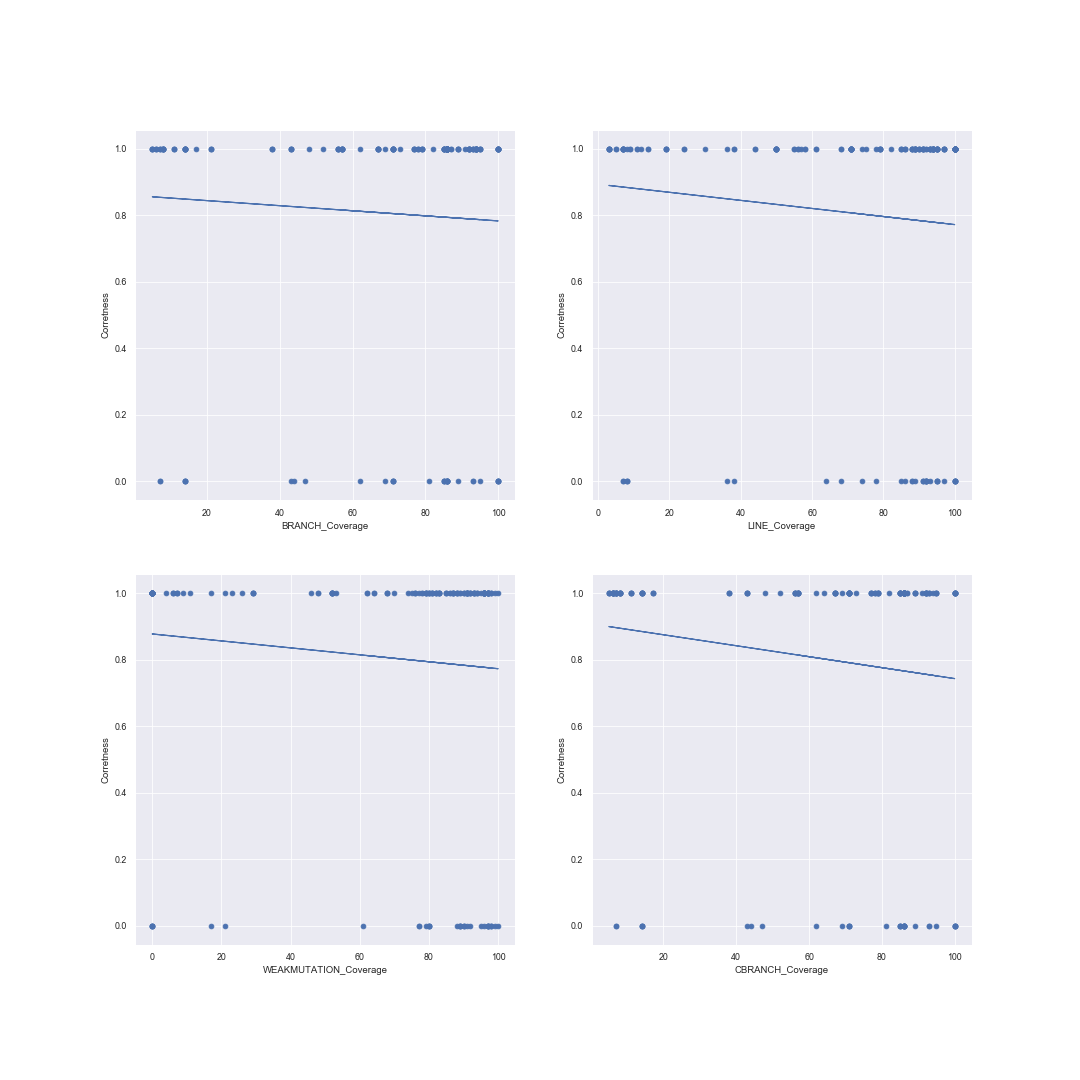
\includegraphics[width=0.8\paperwidth]{q1ScatterValidCorrectness.png}}
    \caption{Plotting the patches against the different coverage metrics, we obtain a series of regression lines for each coverage metric, with p values 0.04, 0.02, 0.08 and 0.07 for branch, line, weakmutation and conditional-branch coverage respectively. There was a positive correlation observed between most test suite coverage metrics and a test suite’s ability to produce patches which do not overfit. Only conditional branch coverage was seen to negatively affect the rate of overfitting. }
    \end{center}
\end{figure}


From Figure 3, we observe that test suites with higher coverage might not necessarily produce patches that are more likely to be correct. In general, however we see that increasing branch coverage, line coverage and weakmutation coverage tended to yield patches which were less likely to overfit. Test suites with higher coverage in those coverage metrics tend to be stronger, and thus more effective in representing program behavior. This potentially leads to less overfitting in the generated patches. 
On the other hand, there was a negative correlation between conditional-branch coverage and the correctness of the patches produced. This means that as conditional-branch coverage of the test suites increased, it was more likely to produce overfitting patches, or at least not more likely to produce non-overfitting patches. This was surprising because in our analysis of test generation metrics, we saw that test suites optimising for conditional branch coverage performed relatively well. One explanation for this phenomenon can be found in the distribution of data points in the scatterplot. A closer look at the data points in the conditional branch and branch plot shows that they mirror each other closely. This is likely because in most cases in the dataset, branches only used 1 conditional statement. Thus, the values obtained for conditional-branch and branch coverage naturally follow each other closely. However, we see that in the plot for conditional-branch coverage,  there are more instances where low conditional-branch coverage values still lead to patches that did not overfit, managing to pass all tests in the evaluation suite. Since conditional-branch coverage is a strict subset of branch coverage, it’s values are always equal to or lower than branch coverage.

\begin{figure}
	\makebox[\textwidth]{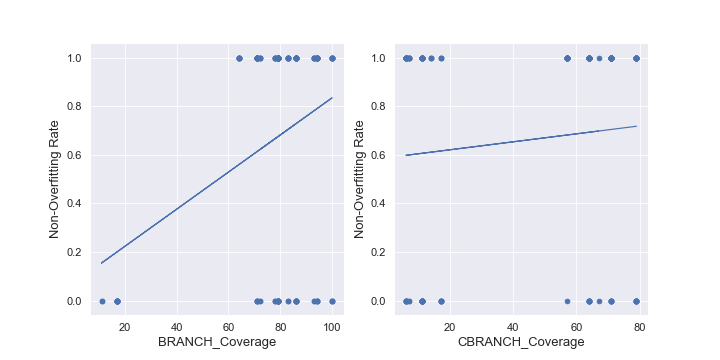
\includegraphics[width=0.8\paperwidth]{q1ScatterValidCorrectnessBranchCBranch.png}}
    \caption{A comparison of only patches generated using test suites for which branch coverage differed from conditional branch coverage. Test suites with low branch coverage almost always produced patches which overfit. Conversely, low conditional-branch coverage still yielded a high rate of patches which did not overfit. Regression lines are used to illustrate the general trend and have p-values of $2.5e-5$ and 0.19 for branch and conditional branch coverage respectively.
}
    \centering
\end{figure}

To investigate the difference, we conducted a study of the 164 patches generated by test suites in which conditional-branch coverage differed from branch coverage. The figure shows that even with test suites with low conditional-branch coverage values, Gin was able to produce non-overfitting patches at least 60\% of the time. In contrast to this, test suites with low branch coverage almost always produced overfitting patches. This emphasises that a fall in conditional-branch coverage has less bearing on overfitting rate and also points to the fact that perhaps the evaluation test suites do not emphasise conditional branch coverage. Across the 11 manual test suites in the dataset, the mean branch coverage was 89\% while the mean conditional-branch coverage was 79\% which might explain this phenomenon. This case study also reinforces the point that test suite metrics are not always accurate predictors of a test suite’s effectiveness, depending on the context. \cite{coveragenotcorrelated}. \\

We can obtain a further look at the relationship between test suite coverage and overfitting in intermediate patches. Intermediate patches are patches which are generated as part of the GI process, but are not returned by the GI process. At every stage, the GI process applies a mutation operator to the current population and records the patch obtained. This new patch is evaluated by the fitness function. Patches which fail to pass some fitness threshold are killed and removed, while the remaining patches are kept and continue to be mutated upon. We refer to the group of patches which pass the fitness threshold at any stage as the intermediate patches. By tracking the growth of these intermediate patches, we can obtain insights into how the final patch returned by the GI process was obtained. Since the final patches represent a small subset of the all patches generated by the GI process, the success of the patch might be obtained by chance. Looking into the intermediate patch data can reinforce our understanding of the trends observed in the final patches.

To conduct this analysis we ran all 11 experiments again, this time recording all the intermediate patches obtained and whether they managed to pass the evaluation suite. Unfortunately, in this version of the experiment, 2 out of the 11 test programs repeatedly took an exceptionally long time to run, exceeding 60 hours. We had no choice but to remove the 2 programs from the experiment. That being said, the remaining dataset still provided a sizable amount of data for us to analyse. In 5760 runs of Gin We managed to obtain 29407 unique intermediate patches. Out of these 29407 patches, 23920 patches were non-empty. We then used these 23920 patches, plotting them as data points on 4 different scatter plots corresponding to each coverage metric based on whether they managed to pass the evaluation test suite.

\begin{figure}
	\makebox[\textwidth]{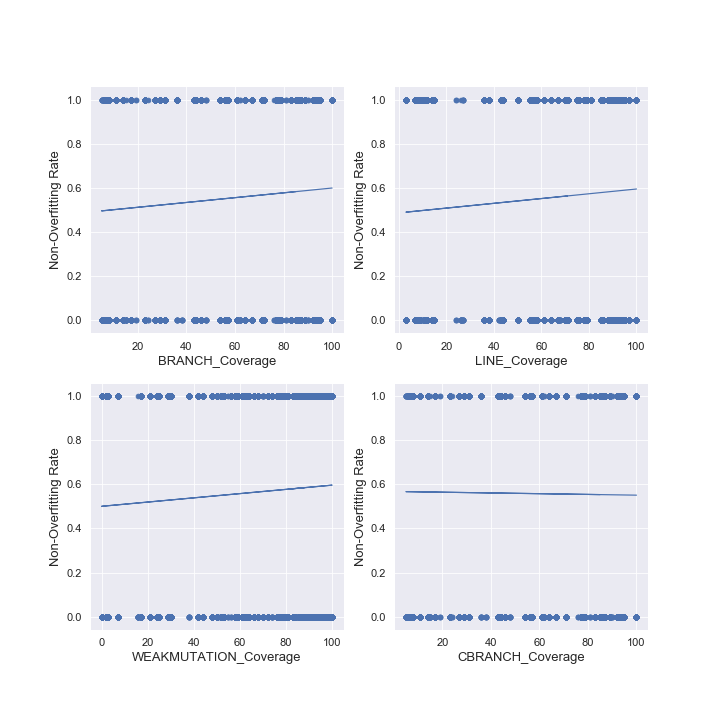
\includegraphics[width=0.8\paperwidth]{q1ScatterIntermediateValidCorrectness.png}}
    \caption{We observe the same broad trends in the intermediate patches as we did in the final patches in Figure 4. However, the correlation between the coverage metrics and overfitting is generally more pronounced, and the non-overfitting rate is higher across the board. All regression lines obtained have p-values of $3.4e-27$, $2.4e-29$, $1.4e-30$ and 0.08 for branch, line, weakmutation and conditional branch coverage respectively}
    \centering
\end{figure}

In Figure 5, we generated a scatterplot for each coverage criterion and used linear regression to obtain a regression line for each coverage metric. Taking a look at the graphs generated, we see that the intermediate patches largely echo the trend seen in the final patches. An increase in branch, line and weakmutation coverage still leads to a lower rate of overfitting, while conditional-branch coverage is still negatively correlated with producing non-overfitting patches, albeit much less so. These findings reinforce our belief that the coverage criteria of test suites still have a large impact on whether generated patches overfit. Moreover, the negative effect of the increase in conditional-branch coverage has been reduced. This is in agreement with our earlier hypothesis that conditional-branch coverage was not actually negatively correlated with the non-overfitting rate. Rather, it was just less highly correlated due to the lack of emphasis on conditional branch coverage in the evaluation suite. 


\subsection{How does test suite generation criterion and coverage metrics of generated tests affect the performance of the generated patches?}

Apart from generating patches which do not overfit, we wanted to assess which criterion would lead to test suites which could generate the most effective patches. In addition to this, we wanted to assess which coverage metric of the generated test suites had the largest impact on the performance of the patches generated. 

With a small search budget, performance improvements were found in all 11 programs using Automated Test suites as input to the process. Out of 1760 runs, Gin managed to produce a patch 381 times. Out of these 381 patches, 98 patches did not overfit, and provided runtime improvements in the evaluation suite. We analysed the runtime improvements provided by these 98 patches by first categorising them by the test suite criterion of the test suite used to generate these patches, and later analysing them based on coverage metrics of these test suites used to generate them.

\begin{figure}
    \begin{center}
        \resizebox{0.8\textwidth}{!}{%% Creator: Matplotlib, PGF backend
%%
%% To include the figure in your LaTeX document, write
%%   \input{<filename>.pgf}
%%
%% Make sure the required packages are loaded in your preamble
%%   \usepackage{pgf}
%%
%% Figures using additional raster images can only be included by \input if
%% they are in the same directory as the main LaTeX file. For loading figures
%% from other directories you can use the `import` package
%%   \usepackage{import}
%% and then include the figures with
%%   \import{<path to file>}{<filename>.pgf}
%%
%% Matplotlib used the following preamble
%%
\begingroup%
\makeatletter%
\begin{pgfpicture}%
\pgfpathrectangle{\pgfpointorigin}{\pgfqpoint{8.000000in}{6.000000in}}%
\pgfusepath{use as bounding box, clip}%
\begin{pgfscope}%
\pgfsetbuttcap%
\pgfsetmiterjoin%
\definecolor{currentfill}{rgb}{1.000000,1.000000,1.000000}%
\pgfsetfillcolor{currentfill}%
\pgfsetlinewidth{0.000000pt}%
\definecolor{currentstroke}{rgb}{1.000000,1.000000,1.000000}%
\pgfsetstrokecolor{currentstroke}%
\pgfsetdash{}{0pt}%
\pgfpathmoveto{\pgfqpoint{0.000000in}{0.000000in}}%
\pgfpathlineto{\pgfqpoint{8.000000in}{0.000000in}}%
\pgfpathlineto{\pgfqpoint{8.000000in}{6.000000in}}%
\pgfpathlineto{\pgfqpoint{0.000000in}{6.000000in}}%
\pgfpathclose%
\pgfusepath{fill}%
\end{pgfscope}%
\begin{pgfscope}%
\pgfsetbuttcap%
\pgfsetmiterjoin%
\definecolor{currentfill}{rgb}{0.917647,0.917647,0.949020}%
\pgfsetfillcolor{currentfill}%
\pgfsetlinewidth{0.000000pt}%
\definecolor{currentstroke}{rgb}{0.000000,0.000000,0.000000}%
\pgfsetstrokecolor{currentstroke}%
\pgfsetstrokeopacity{0.000000}%
\pgfsetdash{}{0pt}%
\pgfpathmoveto{\pgfqpoint{1.000000in}{0.750000in}}%
\pgfpathlineto{\pgfqpoint{7.200000in}{0.750000in}}%
\pgfpathlineto{\pgfqpoint{7.200000in}{5.280000in}}%
\pgfpathlineto{\pgfqpoint{1.000000in}{5.280000in}}%
\pgfpathclose%
\pgfusepath{fill}%
\end{pgfscope}%
\begin{pgfscope}%
\pgfpathrectangle{\pgfqpoint{1.000000in}{0.750000in}}{\pgfqpoint{6.200000in}{4.530000in}}%
\pgfusepath{clip}%
\pgfsetroundcap%
\pgfsetroundjoin%
\pgfsetlinewidth{0.803000pt}%
\definecolor{currentstroke}{rgb}{1.000000,1.000000,1.000000}%
\pgfsetstrokecolor{currentstroke}%
\pgfsetdash{}{0pt}%
\pgfpathmoveto{\pgfqpoint{1.620000in}{0.750000in}}%
\pgfpathlineto{\pgfqpoint{1.620000in}{5.280000in}}%
\pgfusepath{stroke}%
\end{pgfscope}%
\begin{pgfscope}%
\definecolor{textcolor}{rgb}{0.150000,0.150000,0.150000}%
\pgfsetstrokecolor{textcolor}%
\pgfsetfillcolor{textcolor}%
\pgftext[x=1.620000in,y=0.634722in,,top]{\color{textcolor}\rmfamily\fontsize{13.000000}{15.600000}\selectfont Total}%
\end{pgfscope}%
\begin{pgfscope}%
\pgfpathrectangle{\pgfqpoint{1.000000in}{0.750000in}}{\pgfqpoint{6.200000in}{4.530000in}}%
\pgfusepath{clip}%
\pgfsetroundcap%
\pgfsetroundjoin%
\pgfsetlinewidth{0.803000pt}%
\definecolor{currentstroke}{rgb}{1.000000,1.000000,1.000000}%
\pgfsetstrokecolor{currentstroke}%
\pgfsetdash{}{0pt}%
\pgfpathmoveto{\pgfqpoint{2.860000in}{0.750000in}}%
\pgfpathlineto{\pgfqpoint{2.860000in}{5.280000in}}%
\pgfusepath{stroke}%
\end{pgfscope}%
\begin{pgfscope}%
\definecolor{textcolor}{rgb}{0.150000,0.150000,0.150000}%
\pgfsetstrokecolor{textcolor}%
\pgfsetfillcolor{textcolor}%
\pgftext[x=2.860000in,y=0.634722in,,top]{\color{textcolor}\rmfamily\fontsize{13.000000}{15.600000}\selectfont BRANCH}%
\end{pgfscope}%
\begin{pgfscope}%
\pgfpathrectangle{\pgfqpoint{1.000000in}{0.750000in}}{\pgfqpoint{6.200000in}{4.530000in}}%
\pgfusepath{clip}%
\pgfsetroundcap%
\pgfsetroundjoin%
\pgfsetlinewidth{0.803000pt}%
\definecolor{currentstroke}{rgb}{1.000000,1.000000,1.000000}%
\pgfsetstrokecolor{currentstroke}%
\pgfsetdash{}{0pt}%
\pgfpathmoveto{\pgfqpoint{4.100000in}{0.750000in}}%
\pgfpathlineto{\pgfqpoint{4.100000in}{5.280000in}}%
\pgfusepath{stroke}%
\end{pgfscope}%
\begin{pgfscope}%
\definecolor{textcolor}{rgb}{0.150000,0.150000,0.150000}%
\pgfsetstrokecolor{textcolor}%
\pgfsetfillcolor{textcolor}%
\pgftext[x=4.100000in,y=0.634722in,,top]{\color{textcolor}\rmfamily\fontsize{13.000000}{15.600000}\selectfont LINE}%
\end{pgfscope}%
\begin{pgfscope}%
\pgfpathrectangle{\pgfqpoint{1.000000in}{0.750000in}}{\pgfqpoint{6.200000in}{4.530000in}}%
\pgfusepath{clip}%
\pgfsetroundcap%
\pgfsetroundjoin%
\pgfsetlinewidth{0.803000pt}%
\definecolor{currentstroke}{rgb}{1.000000,1.000000,1.000000}%
\pgfsetstrokecolor{currentstroke}%
\pgfsetdash{}{0pt}%
\pgfpathmoveto{\pgfqpoint{5.340000in}{0.750000in}}%
\pgfpathlineto{\pgfqpoint{5.340000in}{5.280000in}}%
\pgfusepath{stroke}%
\end{pgfscope}%
\begin{pgfscope}%
\definecolor{textcolor}{rgb}{0.150000,0.150000,0.150000}%
\pgfsetstrokecolor{textcolor}%
\pgfsetfillcolor{textcolor}%
\pgftext[x=5.340000in,y=0.634722in,,top]{\color{textcolor}\rmfamily\fontsize{13.000000}{15.600000}\selectfont WEAKMUTATION}%
\end{pgfscope}%
\begin{pgfscope}%
\pgfpathrectangle{\pgfqpoint{1.000000in}{0.750000in}}{\pgfqpoint{6.200000in}{4.530000in}}%
\pgfusepath{clip}%
\pgfsetroundcap%
\pgfsetroundjoin%
\pgfsetlinewidth{0.803000pt}%
\definecolor{currentstroke}{rgb}{1.000000,1.000000,1.000000}%
\pgfsetstrokecolor{currentstroke}%
\pgfsetdash{}{0pt}%
\pgfpathmoveto{\pgfqpoint{6.580000in}{0.750000in}}%
\pgfpathlineto{\pgfqpoint{6.580000in}{5.280000in}}%
\pgfusepath{stroke}%
\end{pgfscope}%
\begin{pgfscope}%
\definecolor{textcolor}{rgb}{0.150000,0.150000,0.150000}%
\pgfsetstrokecolor{textcolor}%
\pgfsetfillcolor{textcolor}%
\pgftext[x=6.580000in,y=0.634722in,,top]{\color{textcolor}\rmfamily\fontsize{13.000000}{15.600000}\selectfont CBRANCH}%
\end{pgfscope}%
\begin{pgfscope}%
\definecolor{textcolor}{rgb}{0.150000,0.150000,0.150000}%
\pgfsetstrokecolor{textcolor}%
\pgfsetfillcolor{textcolor}%
\pgftext[x=4.100000in,y=0.431019in,,top]{\color{textcolor}\rmfamily\fontsize{14.000000}{16.800000}\selectfont Test Criterion used for Patch generation}%
\end{pgfscope}%
\begin{pgfscope}%
\pgfpathrectangle{\pgfqpoint{1.000000in}{0.750000in}}{\pgfqpoint{6.200000in}{4.530000in}}%
\pgfusepath{clip}%
\pgfsetroundcap%
\pgfsetroundjoin%
\pgfsetlinewidth{0.803000pt}%
\definecolor{currentstroke}{rgb}{1.000000,1.000000,1.000000}%
\pgfsetstrokecolor{currentstroke}%
\pgfsetdash{}{0pt}%
\pgfpathmoveto{\pgfqpoint{1.000000in}{1.305495in}}%
\pgfpathlineto{\pgfqpoint{7.200000in}{1.305495in}}%
\pgfusepath{stroke}%
\end{pgfscope}%
\begin{pgfscope}%
\definecolor{textcolor}{rgb}{0.150000,0.150000,0.150000}%
\pgfsetstrokecolor{textcolor}%
\pgfsetfillcolor{textcolor}%
\pgftext[x=0.803126in,y=1.247625in,left,base]{\color{textcolor}\rmfamily\fontsize{13.000000}{15.600000}\selectfont \(\displaystyle 0\)}%
\end{pgfscope}%
\begin{pgfscope}%
\pgfpathrectangle{\pgfqpoint{1.000000in}{0.750000in}}{\pgfqpoint{6.200000in}{4.530000in}}%
\pgfusepath{clip}%
\pgfsetroundcap%
\pgfsetroundjoin%
\pgfsetlinewidth{0.803000pt}%
\definecolor{currentstroke}{rgb}{1.000000,1.000000,1.000000}%
\pgfsetstrokecolor{currentstroke}%
\pgfsetdash{}{0pt}%
\pgfpathmoveto{\pgfqpoint{1.000000in}{2.067338in}}%
\pgfpathlineto{\pgfqpoint{7.200000in}{2.067338in}}%
\pgfusepath{stroke}%
\end{pgfscope}%
\begin{pgfscope}%
\definecolor{textcolor}{rgb}{0.150000,0.150000,0.150000}%
\pgfsetstrokecolor{textcolor}%
\pgfsetfillcolor{textcolor}%
\pgftext[x=0.721529in,y=2.009468in,left,base]{\color{textcolor}\rmfamily\fontsize{13.000000}{15.600000}\selectfont \(\displaystyle 20\)}%
\end{pgfscope}%
\begin{pgfscope}%
\pgfpathrectangle{\pgfqpoint{1.000000in}{0.750000in}}{\pgfqpoint{6.200000in}{4.530000in}}%
\pgfusepath{clip}%
\pgfsetroundcap%
\pgfsetroundjoin%
\pgfsetlinewidth{0.803000pt}%
\definecolor{currentstroke}{rgb}{1.000000,1.000000,1.000000}%
\pgfsetstrokecolor{currentstroke}%
\pgfsetdash{}{0pt}%
\pgfpathmoveto{\pgfqpoint{1.000000in}{2.829182in}}%
\pgfpathlineto{\pgfqpoint{7.200000in}{2.829182in}}%
\pgfusepath{stroke}%
\end{pgfscope}%
\begin{pgfscope}%
\definecolor{textcolor}{rgb}{0.150000,0.150000,0.150000}%
\pgfsetstrokecolor{textcolor}%
\pgfsetfillcolor{textcolor}%
\pgftext[x=0.721529in,y=2.771312in,left,base]{\color{textcolor}\rmfamily\fontsize{13.000000}{15.600000}\selectfont \(\displaystyle 40\)}%
\end{pgfscope}%
\begin{pgfscope}%
\pgfpathrectangle{\pgfqpoint{1.000000in}{0.750000in}}{\pgfqpoint{6.200000in}{4.530000in}}%
\pgfusepath{clip}%
\pgfsetroundcap%
\pgfsetroundjoin%
\pgfsetlinewidth{0.803000pt}%
\definecolor{currentstroke}{rgb}{1.000000,1.000000,1.000000}%
\pgfsetstrokecolor{currentstroke}%
\pgfsetdash{}{0pt}%
\pgfpathmoveto{\pgfqpoint{1.000000in}{3.591025in}}%
\pgfpathlineto{\pgfqpoint{7.200000in}{3.591025in}}%
\pgfusepath{stroke}%
\end{pgfscope}%
\begin{pgfscope}%
\definecolor{textcolor}{rgb}{0.150000,0.150000,0.150000}%
\pgfsetstrokecolor{textcolor}%
\pgfsetfillcolor{textcolor}%
\pgftext[x=0.721529in,y=3.533155in,left,base]{\color{textcolor}\rmfamily\fontsize{13.000000}{15.600000}\selectfont \(\displaystyle 60\)}%
\end{pgfscope}%
\begin{pgfscope}%
\pgfpathrectangle{\pgfqpoint{1.000000in}{0.750000in}}{\pgfqpoint{6.200000in}{4.530000in}}%
\pgfusepath{clip}%
\pgfsetroundcap%
\pgfsetroundjoin%
\pgfsetlinewidth{0.803000pt}%
\definecolor{currentstroke}{rgb}{1.000000,1.000000,1.000000}%
\pgfsetstrokecolor{currentstroke}%
\pgfsetdash{}{0pt}%
\pgfpathmoveto{\pgfqpoint{1.000000in}{4.352869in}}%
\pgfpathlineto{\pgfqpoint{7.200000in}{4.352869in}}%
\pgfusepath{stroke}%
\end{pgfscope}%
\begin{pgfscope}%
\definecolor{textcolor}{rgb}{0.150000,0.150000,0.150000}%
\pgfsetstrokecolor{textcolor}%
\pgfsetfillcolor{textcolor}%
\pgftext[x=0.721529in,y=4.294998in,left,base]{\color{textcolor}\rmfamily\fontsize{13.000000}{15.600000}\selectfont \(\displaystyle 80\)}%
\end{pgfscope}%
\begin{pgfscope}%
\pgfpathrectangle{\pgfqpoint{1.000000in}{0.750000in}}{\pgfqpoint{6.200000in}{4.530000in}}%
\pgfusepath{clip}%
\pgfsetroundcap%
\pgfsetroundjoin%
\pgfsetlinewidth{0.803000pt}%
\definecolor{currentstroke}{rgb}{1.000000,1.000000,1.000000}%
\pgfsetstrokecolor{currentstroke}%
\pgfsetdash{}{0pt}%
\pgfpathmoveto{\pgfqpoint{1.000000in}{5.114712in}}%
\pgfpathlineto{\pgfqpoint{7.200000in}{5.114712in}}%
\pgfusepath{stroke}%
\end{pgfscope}%
\begin{pgfscope}%
\definecolor{textcolor}{rgb}{0.150000,0.150000,0.150000}%
\pgfsetstrokecolor{textcolor}%
\pgfsetfillcolor{textcolor}%
\pgftext[x=0.639933in,y=5.056842in,left,base]{\color{textcolor}\rmfamily\fontsize{13.000000}{15.600000}\selectfont \(\displaystyle 100\)}%
\end{pgfscope}%
\begin{pgfscope}%
\definecolor{textcolor}{rgb}{0.150000,0.150000,0.150000}%
\pgfsetstrokecolor{textcolor}%
\pgfsetfillcolor{textcolor}%
\pgftext[x=0.584377in,y=3.015000in,,bottom,rotate=90.000000]{\color{textcolor}\rmfamily\fontsize{14.000000}{16.800000}\selectfont \% Speedup on evaluation test}%
\end{pgfscope}%
\begin{pgfscope}%
\pgfpathrectangle{\pgfqpoint{1.000000in}{0.750000in}}{\pgfqpoint{6.200000in}{4.530000in}}%
\pgfusepath{clip}%
\pgfsetroundcap%
\pgfsetroundjoin%
\pgfsetlinewidth{1.003750pt}%
\definecolor{currentstroke}{rgb}{0.000000,0.000000,0.000000}%
\pgfsetstrokecolor{currentstroke}%
\pgfsetdash{}{0pt}%
\pgfpathmoveto{\pgfqpoint{1.310000in}{1.314672in}}%
\pgfpathlineto{\pgfqpoint{1.930000in}{1.314672in}}%
\pgfpathlineto{\pgfqpoint{1.930000in}{2.973756in}}%
\pgfpathlineto{\pgfqpoint{1.310000in}{2.973756in}}%
\pgfpathlineto{\pgfqpoint{1.310000in}{1.314672in}}%
\pgfusepath{stroke}%
\end{pgfscope}%
\begin{pgfscope}%
\pgfpathrectangle{\pgfqpoint{1.000000in}{0.750000in}}{\pgfqpoint{6.200000in}{4.530000in}}%
\pgfusepath{clip}%
\pgfsetroundcap%
\pgfsetroundjoin%
\pgfsetlinewidth{1.003750pt}%
\definecolor{currentstroke}{rgb}{0.000000,0.000000,0.000000}%
\pgfsetstrokecolor{currentstroke}%
\pgfsetdash{}{0pt}%
\pgfpathmoveto{\pgfqpoint{1.620000in}{1.314672in}}%
\pgfpathlineto{\pgfqpoint{1.620000in}{0.955909in}}%
\pgfusepath{stroke}%
\end{pgfscope}%
\begin{pgfscope}%
\pgfpathrectangle{\pgfqpoint{1.000000in}{0.750000in}}{\pgfqpoint{6.200000in}{4.530000in}}%
\pgfusepath{clip}%
\pgfsetroundcap%
\pgfsetroundjoin%
\pgfsetlinewidth{1.003750pt}%
\definecolor{currentstroke}{rgb}{0.000000,0.000000,0.000000}%
\pgfsetstrokecolor{currentstroke}%
\pgfsetdash{}{0pt}%
\pgfpathmoveto{\pgfqpoint{1.620000in}{2.973756in}}%
\pgfpathlineto{\pgfqpoint{1.620000in}{5.074091in}}%
\pgfusepath{stroke}%
\end{pgfscope}%
\begin{pgfscope}%
\pgfpathrectangle{\pgfqpoint{1.000000in}{0.750000in}}{\pgfqpoint{6.200000in}{4.530000in}}%
\pgfusepath{clip}%
\pgfsetroundcap%
\pgfsetroundjoin%
\pgfsetlinewidth{1.003750pt}%
\definecolor{currentstroke}{rgb}{0.000000,0.000000,0.000000}%
\pgfsetstrokecolor{currentstroke}%
\pgfsetdash{}{0pt}%
\pgfpathmoveto{\pgfqpoint{1.465000in}{0.955909in}}%
\pgfpathlineto{\pgfqpoint{1.775000in}{0.955909in}}%
\pgfusepath{stroke}%
\end{pgfscope}%
\begin{pgfscope}%
\pgfpathrectangle{\pgfqpoint{1.000000in}{0.750000in}}{\pgfqpoint{6.200000in}{4.530000in}}%
\pgfusepath{clip}%
\pgfsetroundcap%
\pgfsetroundjoin%
\pgfsetlinewidth{1.003750pt}%
\definecolor{currentstroke}{rgb}{0.000000,0.000000,0.000000}%
\pgfsetstrokecolor{currentstroke}%
\pgfsetdash{}{0pt}%
\pgfpathmoveto{\pgfqpoint{1.465000in}{5.074091in}}%
\pgfpathlineto{\pgfqpoint{1.775000in}{5.074091in}}%
\pgfusepath{stroke}%
\end{pgfscope}%
\begin{pgfscope}%
\pgfpathrectangle{\pgfqpoint{1.000000in}{0.750000in}}{\pgfqpoint{6.200000in}{4.530000in}}%
\pgfusepath{clip}%
\pgfsetroundcap%
\pgfsetroundjoin%
\pgfsetlinewidth{1.003750pt}%
\definecolor{currentstroke}{rgb}{0.000000,0.000000,0.000000}%
\pgfsetstrokecolor{currentstroke}%
\pgfsetdash{}{0pt}%
\pgfpathmoveto{\pgfqpoint{2.550000in}{1.679442in}}%
\pgfpathlineto{\pgfqpoint{3.170000in}{1.679442in}}%
\pgfpathlineto{\pgfqpoint{3.170000in}{3.252907in}}%
\pgfpathlineto{\pgfqpoint{2.550000in}{3.252907in}}%
\pgfpathlineto{\pgfqpoint{2.550000in}{1.679442in}}%
\pgfusepath{stroke}%
\end{pgfscope}%
\begin{pgfscope}%
\pgfpathrectangle{\pgfqpoint{1.000000in}{0.750000in}}{\pgfqpoint{6.200000in}{4.530000in}}%
\pgfusepath{clip}%
\pgfsetroundcap%
\pgfsetroundjoin%
\pgfsetlinewidth{1.003750pt}%
\definecolor{currentstroke}{rgb}{0.000000,0.000000,0.000000}%
\pgfsetstrokecolor{currentstroke}%
\pgfsetdash{}{0pt}%
\pgfpathmoveto{\pgfqpoint{2.860000in}{1.679442in}}%
\pgfpathlineto{\pgfqpoint{2.860000in}{1.149499in}}%
\pgfusepath{stroke}%
\end{pgfscope}%
\begin{pgfscope}%
\pgfpathrectangle{\pgfqpoint{1.000000in}{0.750000in}}{\pgfqpoint{6.200000in}{4.530000in}}%
\pgfusepath{clip}%
\pgfsetroundcap%
\pgfsetroundjoin%
\pgfsetlinewidth{1.003750pt}%
\definecolor{currentstroke}{rgb}{0.000000,0.000000,0.000000}%
\pgfsetstrokecolor{currentstroke}%
\pgfsetdash{}{0pt}%
\pgfpathmoveto{\pgfqpoint{2.860000in}{3.252907in}}%
\pgfpathlineto{\pgfqpoint{2.860000in}{5.074091in}}%
\pgfusepath{stroke}%
\end{pgfscope}%
\begin{pgfscope}%
\pgfpathrectangle{\pgfqpoint{1.000000in}{0.750000in}}{\pgfqpoint{6.200000in}{4.530000in}}%
\pgfusepath{clip}%
\pgfsetroundcap%
\pgfsetroundjoin%
\pgfsetlinewidth{1.003750pt}%
\definecolor{currentstroke}{rgb}{0.000000,0.000000,0.000000}%
\pgfsetstrokecolor{currentstroke}%
\pgfsetdash{}{0pt}%
\pgfpathmoveto{\pgfqpoint{2.705000in}{1.149499in}}%
\pgfpathlineto{\pgfqpoint{3.015000in}{1.149499in}}%
\pgfusepath{stroke}%
\end{pgfscope}%
\begin{pgfscope}%
\pgfpathrectangle{\pgfqpoint{1.000000in}{0.750000in}}{\pgfqpoint{6.200000in}{4.530000in}}%
\pgfusepath{clip}%
\pgfsetroundcap%
\pgfsetroundjoin%
\pgfsetlinewidth{1.003750pt}%
\definecolor{currentstroke}{rgb}{0.000000,0.000000,0.000000}%
\pgfsetstrokecolor{currentstroke}%
\pgfsetdash{}{0pt}%
\pgfpathmoveto{\pgfqpoint{2.705000in}{5.074091in}}%
\pgfpathlineto{\pgfqpoint{3.015000in}{5.074091in}}%
\pgfusepath{stroke}%
\end{pgfscope}%
\begin{pgfscope}%
\pgfpathrectangle{\pgfqpoint{1.000000in}{0.750000in}}{\pgfqpoint{6.200000in}{4.530000in}}%
\pgfusepath{clip}%
\pgfsetroundcap%
\pgfsetroundjoin%
\pgfsetlinewidth{1.003750pt}%
\definecolor{currentstroke}{rgb}{0.000000,0.000000,0.000000}%
\pgfsetstrokecolor{currentstroke}%
\pgfsetdash{}{0pt}%
\pgfpathmoveto{\pgfqpoint{3.790000in}{1.240310in}}%
\pgfpathlineto{\pgfqpoint{4.410000in}{1.240310in}}%
\pgfpathlineto{\pgfqpoint{4.410000in}{2.691856in}}%
\pgfpathlineto{\pgfqpoint{3.790000in}{2.691856in}}%
\pgfpathlineto{\pgfqpoint{3.790000in}{1.240310in}}%
\pgfusepath{stroke}%
\end{pgfscope}%
\begin{pgfscope}%
\pgfpathrectangle{\pgfqpoint{1.000000in}{0.750000in}}{\pgfqpoint{6.200000in}{4.530000in}}%
\pgfusepath{clip}%
\pgfsetroundcap%
\pgfsetroundjoin%
\pgfsetlinewidth{1.003750pt}%
\definecolor{currentstroke}{rgb}{0.000000,0.000000,0.000000}%
\pgfsetstrokecolor{currentstroke}%
\pgfsetdash{}{0pt}%
\pgfpathmoveto{\pgfqpoint{4.100000in}{1.240310in}}%
\pgfpathlineto{\pgfqpoint{4.100000in}{0.955909in}}%
\pgfusepath{stroke}%
\end{pgfscope}%
\begin{pgfscope}%
\pgfpathrectangle{\pgfqpoint{1.000000in}{0.750000in}}{\pgfqpoint{6.200000in}{4.530000in}}%
\pgfusepath{clip}%
\pgfsetroundcap%
\pgfsetroundjoin%
\pgfsetlinewidth{1.003750pt}%
\definecolor{currentstroke}{rgb}{0.000000,0.000000,0.000000}%
\pgfsetstrokecolor{currentstroke}%
\pgfsetdash{}{0pt}%
\pgfpathmoveto{\pgfqpoint{4.100000in}{2.691856in}}%
\pgfpathlineto{\pgfqpoint{4.100000in}{3.495425in}}%
\pgfusepath{stroke}%
\end{pgfscope}%
\begin{pgfscope}%
\pgfpathrectangle{\pgfqpoint{1.000000in}{0.750000in}}{\pgfqpoint{6.200000in}{4.530000in}}%
\pgfusepath{clip}%
\pgfsetroundcap%
\pgfsetroundjoin%
\pgfsetlinewidth{1.003750pt}%
\definecolor{currentstroke}{rgb}{0.000000,0.000000,0.000000}%
\pgfsetstrokecolor{currentstroke}%
\pgfsetdash{}{0pt}%
\pgfpathmoveto{\pgfqpoint{3.945000in}{0.955909in}}%
\pgfpathlineto{\pgfqpoint{4.255000in}{0.955909in}}%
\pgfusepath{stroke}%
\end{pgfscope}%
\begin{pgfscope}%
\pgfpathrectangle{\pgfqpoint{1.000000in}{0.750000in}}{\pgfqpoint{6.200000in}{4.530000in}}%
\pgfusepath{clip}%
\pgfsetroundcap%
\pgfsetroundjoin%
\pgfsetlinewidth{1.003750pt}%
\definecolor{currentstroke}{rgb}{0.000000,0.000000,0.000000}%
\pgfsetstrokecolor{currentstroke}%
\pgfsetdash{}{0pt}%
\pgfpathmoveto{\pgfqpoint{3.945000in}{3.495425in}}%
\pgfpathlineto{\pgfqpoint{4.255000in}{3.495425in}}%
\pgfusepath{stroke}%
\end{pgfscope}%
\begin{pgfscope}%
\pgfpathrectangle{\pgfqpoint{1.000000in}{0.750000in}}{\pgfqpoint{6.200000in}{4.530000in}}%
\pgfusepath{clip}%
\pgfsetroundcap%
\pgfsetroundjoin%
\pgfsetlinewidth{1.003750pt}%
\definecolor{currentstroke}{rgb}{0.000000,0.000000,0.000000}%
\pgfsetstrokecolor{currentstroke}%
\pgfsetdash{}{0pt}%
\pgfpathmoveto{\pgfqpoint{5.030000in}{1.315659in}}%
\pgfpathlineto{\pgfqpoint{5.650000in}{1.315659in}}%
\pgfpathlineto{\pgfqpoint{5.650000in}{3.182185in}}%
\pgfpathlineto{\pgfqpoint{5.030000in}{3.182185in}}%
\pgfpathlineto{\pgfqpoint{5.030000in}{1.315659in}}%
\pgfusepath{stroke}%
\end{pgfscope}%
\begin{pgfscope}%
\pgfpathrectangle{\pgfqpoint{1.000000in}{0.750000in}}{\pgfqpoint{6.200000in}{4.530000in}}%
\pgfusepath{clip}%
\pgfsetroundcap%
\pgfsetroundjoin%
\pgfsetlinewidth{1.003750pt}%
\definecolor{currentstroke}{rgb}{0.000000,0.000000,0.000000}%
\pgfsetstrokecolor{currentstroke}%
\pgfsetdash{}{0pt}%
\pgfpathmoveto{\pgfqpoint{5.340000in}{1.315659in}}%
\pgfpathlineto{\pgfqpoint{5.340000in}{1.099644in}}%
\pgfusepath{stroke}%
\end{pgfscope}%
\begin{pgfscope}%
\pgfpathrectangle{\pgfqpoint{1.000000in}{0.750000in}}{\pgfqpoint{6.200000in}{4.530000in}}%
\pgfusepath{clip}%
\pgfsetroundcap%
\pgfsetroundjoin%
\pgfsetlinewidth{1.003750pt}%
\definecolor{currentstroke}{rgb}{0.000000,0.000000,0.000000}%
\pgfsetstrokecolor{currentstroke}%
\pgfsetdash{}{0pt}%
\pgfpathmoveto{\pgfqpoint{5.340000in}{3.182185in}}%
\pgfpathlineto{\pgfqpoint{5.340000in}{5.055538in}}%
\pgfusepath{stroke}%
\end{pgfscope}%
\begin{pgfscope}%
\pgfpathrectangle{\pgfqpoint{1.000000in}{0.750000in}}{\pgfqpoint{6.200000in}{4.530000in}}%
\pgfusepath{clip}%
\pgfsetroundcap%
\pgfsetroundjoin%
\pgfsetlinewidth{1.003750pt}%
\definecolor{currentstroke}{rgb}{0.000000,0.000000,0.000000}%
\pgfsetstrokecolor{currentstroke}%
\pgfsetdash{}{0pt}%
\pgfpathmoveto{\pgfqpoint{5.185000in}{1.099644in}}%
\pgfpathlineto{\pgfqpoint{5.495000in}{1.099644in}}%
\pgfusepath{stroke}%
\end{pgfscope}%
\begin{pgfscope}%
\pgfpathrectangle{\pgfqpoint{1.000000in}{0.750000in}}{\pgfqpoint{6.200000in}{4.530000in}}%
\pgfusepath{clip}%
\pgfsetroundcap%
\pgfsetroundjoin%
\pgfsetlinewidth{1.003750pt}%
\definecolor{currentstroke}{rgb}{0.000000,0.000000,0.000000}%
\pgfsetstrokecolor{currentstroke}%
\pgfsetdash{}{0pt}%
\pgfpathmoveto{\pgfqpoint{5.185000in}{5.055538in}}%
\pgfpathlineto{\pgfqpoint{5.495000in}{5.055538in}}%
\pgfusepath{stroke}%
\end{pgfscope}%
\begin{pgfscope}%
\pgfpathrectangle{\pgfqpoint{1.000000in}{0.750000in}}{\pgfqpoint{6.200000in}{4.530000in}}%
\pgfusepath{clip}%
\pgfsetroundcap%
\pgfsetroundjoin%
\pgfsetlinewidth{1.003750pt}%
\definecolor{currentstroke}{rgb}{0.000000,0.000000,0.000000}%
\pgfsetstrokecolor{currentstroke}%
\pgfsetdash{}{0pt}%
\pgfpathmoveto{\pgfqpoint{6.270000in}{1.298273in}}%
\pgfpathlineto{\pgfqpoint{6.890000in}{1.298273in}}%
\pgfpathlineto{\pgfqpoint{6.890000in}{1.836748in}}%
\pgfpathlineto{\pgfqpoint{6.270000in}{1.836748in}}%
\pgfpathlineto{\pgfqpoint{6.270000in}{1.298273in}}%
\pgfusepath{stroke}%
\end{pgfscope}%
\begin{pgfscope}%
\pgfpathrectangle{\pgfqpoint{1.000000in}{0.750000in}}{\pgfqpoint{6.200000in}{4.530000in}}%
\pgfusepath{clip}%
\pgfsetroundcap%
\pgfsetroundjoin%
\pgfsetlinewidth{1.003750pt}%
\definecolor{currentstroke}{rgb}{0.000000,0.000000,0.000000}%
\pgfsetstrokecolor{currentstroke}%
\pgfsetdash{}{0pt}%
\pgfpathmoveto{\pgfqpoint{6.580000in}{1.298273in}}%
\pgfpathlineto{\pgfqpoint{6.580000in}{1.018921in}}%
\pgfusepath{stroke}%
\end{pgfscope}%
\begin{pgfscope}%
\pgfpathrectangle{\pgfqpoint{1.000000in}{0.750000in}}{\pgfqpoint{6.200000in}{4.530000in}}%
\pgfusepath{clip}%
\pgfsetroundcap%
\pgfsetroundjoin%
\pgfsetlinewidth{1.003750pt}%
\definecolor{currentstroke}{rgb}{0.000000,0.000000,0.000000}%
\pgfsetstrokecolor{currentstroke}%
\pgfsetdash{}{0pt}%
\pgfpathmoveto{\pgfqpoint{6.580000in}{1.836748in}}%
\pgfpathlineto{\pgfqpoint{6.580000in}{2.631165in}}%
\pgfusepath{stroke}%
\end{pgfscope}%
\begin{pgfscope}%
\pgfpathrectangle{\pgfqpoint{1.000000in}{0.750000in}}{\pgfqpoint{6.200000in}{4.530000in}}%
\pgfusepath{clip}%
\pgfsetroundcap%
\pgfsetroundjoin%
\pgfsetlinewidth{1.003750pt}%
\definecolor{currentstroke}{rgb}{0.000000,0.000000,0.000000}%
\pgfsetstrokecolor{currentstroke}%
\pgfsetdash{}{0pt}%
\pgfpathmoveto{\pgfqpoint{6.425000in}{1.018921in}}%
\pgfpathlineto{\pgfqpoint{6.735000in}{1.018921in}}%
\pgfusepath{stroke}%
\end{pgfscope}%
\begin{pgfscope}%
\pgfpathrectangle{\pgfqpoint{1.000000in}{0.750000in}}{\pgfqpoint{6.200000in}{4.530000in}}%
\pgfusepath{clip}%
\pgfsetroundcap%
\pgfsetroundjoin%
\pgfsetlinewidth{1.003750pt}%
\definecolor{currentstroke}{rgb}{0.000000,0.000000,0.000000}%
\pgfsetstrokecolor{currentstroke}%
\pgfsetdash{}{0pt}%
\pgfpathmoveto{\pgfqpoint{6.425000in}{2.631165in}}%
\pgfpathlineto{\pgfqpoint{6.735000in}{2.631165in}}%
\pgfusepath{stroke}%
\end{pgfscope}%
\begin{pgfscope}%
\pgfpathrectangle{\pgfqpoint{1.000000in}{0.750000in}}{\pgfqpoint{6.200000in}{4.530000in}}%
\pgfusepath{clip}%
\pgfsetroundcap%
\pgfsetroundjoin%
\pgfsetlinewidth{1.003750pt}%
\definecolor{currentstroke}{rgb}{0.866667,0.517647,0.321569}%
\pgfsetstrokecolor{currentstroke}%
\pgfsetdash{}{0pt}%
\pgfpathmoveto{\pgfqpoint{1.310000in}{1.750371in}}%
\pgfpathlineto{\pgfqpoint{1.930000in}{1.750371in}}%
\pgfusepath{stroke}%
\end{pgfscope}%
\begin{pgfscope}%
\pgfpathrectangle{\pgfqpoint{1.000000in}{0.750000in}}{\pgfqpoint{6.200000in}{4.530000in}}%
\pgfusepath{clip}%
\pgfsetroundcap%
\pgfsetroundjoin%
\pgfsetlinewidth{1.003750pt}%
\definecolor{currentstroke}{rgb}{0.866667,0.517647,0.321569}%
\pgfsetstrokecolor{currentstroke}%
\pgfsetdash{}{0pt}%
\pgfpathmoveto{\pgfqpoint{2.550000in}{2.704649in}}%
\pgfpathlineto{\pgfqpoint{3.170000in}{2.704649in}}%
\pgfusepath{stroke}%
\end{pgfscope}%
\begin{pgfscope}%
\pgfpathrectangle{\pgfqpoint{1.000000in}{0.750000in}}{\pgfqpoint{6.200000in}{4.530000in}}%
\pgfusepath{clip}%
\pgfsetroundcap%
\pgfsetroundjoin%
\pgfsetlinewidth{1.003750pt}%
\definecolor{currentstroke}{rgb}{0.866667,0.517647,0.321569}%
\pgfsetstrokecolor{currentstroke}%
\pgfsetdash{}{0pt}%
\pgfpathmoveto{\pgfqpoint{3.790000in}{1.702964in}}%
\pgfpathlineto{\pgfqpoint{4.410000in}{1.702964in}}%
\pgfusepath{stroke}%
\end{pgfscope}%
\begin{pgfscope}%
\pgfpathrectangle{\pgfqpoint{1.000000in}{0.750000in}}{\pgfqpoint{6.200000in}{4.530000in}}%
\pgfusepath{clip}%
\pgfsetroundcap%
\pgfsetroundjoin%
\pgfsetlinewidth{1.003750pt}%
\definecolor{currentstroke}{rgb}{0.866667,0.517647,0.321569}%
\pgfsetstrokecolor{currentstroke}%
\pgfsetdash{}{0pt}%
\pgfpathmoveto{\pgfqpoint{5.030000in}{1.520206in}}%
\pgfpathlineto{\pgfqpoint{5.650000in}{1.520206in}}%
\pgfusepath{stroke}%
\end{pgfscope}%
\begin{pgfscope}%
\pgfpathrectangle{\pgfqpoint{1.000000in}{0.750000in}}{\pgfqpoint{6.200000in}{4.530000in}}%
\pgfusepath{clip}%
\pgfsetroundcap%
\pgfsetroundjoin%
\pgfsetlinewidth{1.003750pt}%
\definecolor{currentstroke}{rgb}{0.866667,0.517647,0.321569}%
\pgfsetstrokecolor{currentstroke}%
\pgfsetdash{}{0pt}%
\pgfpathmoveto{\pgfqpoint{6.270000in}{1.418770in}}%
\pgfpathlineto{\pgfqpoint{6.890000in}{1.418770in}}%
\pgfusepath{stroke}%
\end{pgfscope}%
\begin{pgfscope}%
\pgfsetrectcap%
\pgfsetmiterjoin%
\pgfsetlinewidth{1.003750pt}%
\definecolor{currentstroke}{rgb}{1.000000,1.000000,1.000000}%
\pgfsetstrokecolor{currentstroke}%
\pgfsetdash{}{0pt}%
\pgfpathmoveto{\pgfqpoint{1.000000in}{0.750000in}}%
\pgfpathlineto{\pgfqpoint{1.000000in}{5.280000in}}%
\pgfusepath{stroke}%
\end{pgfscope}%
\begin{pgfscope}%
\pgfsetrectcap%
\pgfsetmiterjoin%
\pgfsetlinewidth{1.003750pt}%
\definecolor{currentstroke}{rgb}{1.000000,1.000000,1.000000}%
\pgfsetstrokecolor{currentstroke}%
\pgfsetdash{}{0pt}%
\pgfpathmoveto{\pgfqpoint{7.200000in}{0.750000in}}%
\pgfpathlineto{\pgfqpoint{7.200000in}{5.280000in}}%
\pgfusepath{stroke}%
\end{pgfscope}%
\begin{pgfscope}%
\pgfsetrectcap%
\pgfsetmiterjoin%
\pgfsetlinewidth{1.003750pt}%
\definecolor{currentstroke}{rgb}{1.000000,1.000000,1.000000}%
\pgfsetstrokecolor{currentstroke}%
\pgfsetdash{}{0pt}%
\pgfpathmoveto{\pgfqpoint{1.000000in}{0.750000in}}%
\pgfpathlineto{\pgfqpoint{7.200000in}{0.750000in}}%
\pgfusepath{stroke}%
\end{pgfscope}%
\begin{pgfscope}%
\pgfsetrectcap%
\pgfsetmiterjoin%
\pgfsetlinewidth{1.003750pt}%
\definecolor{currentstroke}{rgb}{1.000000,1.000000,1.000000}%
\pgfsetstrokecolor{currentstroke}%
\pgfsetdash{}{0pt}%
\pgfpathmoveto{\pgfqpoint{1.000000in}{5.280000in}}%
\pgfpathlineto{\pgfqpoint{7.200000in}{5.280000in}}%
\pgfusepath{stroke}%
\end{pgfscope}%
\end{pgfpicture}%
\makeatother%
\endgroup%
}
    \end{center}
    \caption{Test suites optimising for branch coverage produced patches which showed the highest mean speedup\% by far at 38\% with a standard deviation of 34.5\%.  Test suites optimising for conditional branch coverage produced patches which provided the least improvements at a mean of 13.2\%, but with the smallest standard variation at 25.8\%. Automated test suites optimised for branch coverage showed an increase in performance compared to other test suite criteria, with a p-value of 0.01.
}
\end{figure}

Figure 6 shows a boxplot which illustrates the performance of patches generated with each test criterion. The boxed regions signify the upper and lower quartiles of the recorded speedup, while the whiskers show the range of values taken by patches. All non-overfitting patches were considered in this study.

The first thing to note here is that the reduction in runtime varies by a large amount. This is to be expected since the genetic improvement process is a non-deterministic process and the space of available patches is huge. This leads to a large variation in the performance improvements that can be obtained with each patch.

Despite this large variance in improvement, patches generated with test suites optimised for branch coverage provide the highest median speedup by far among all test case criterion with a median of 38\%.  Alongside the results from part 6.1, where test suites which optimised for branch coverage also managed to produce the highest proportion of non-overfitting tests, branch coverage seems to be a promising candidate for optimising the genetic improvement process. While in the GI process, the test suite merely serves to provide an automated way to check for overfitting, a large improvement in performance could indicate that the test suite allows for sufficient exploration of the search space, allowing the process to find optimal solutions more quickly. The high performance of test suites optimised for Branch coverage in this study might point to its effectiveness in both providing strong test suites which limit overfitting, while allowing sufficient flexibility such that good optimisations are still being able to be found.

\begin{figure}
	\makebox[\textwidth]{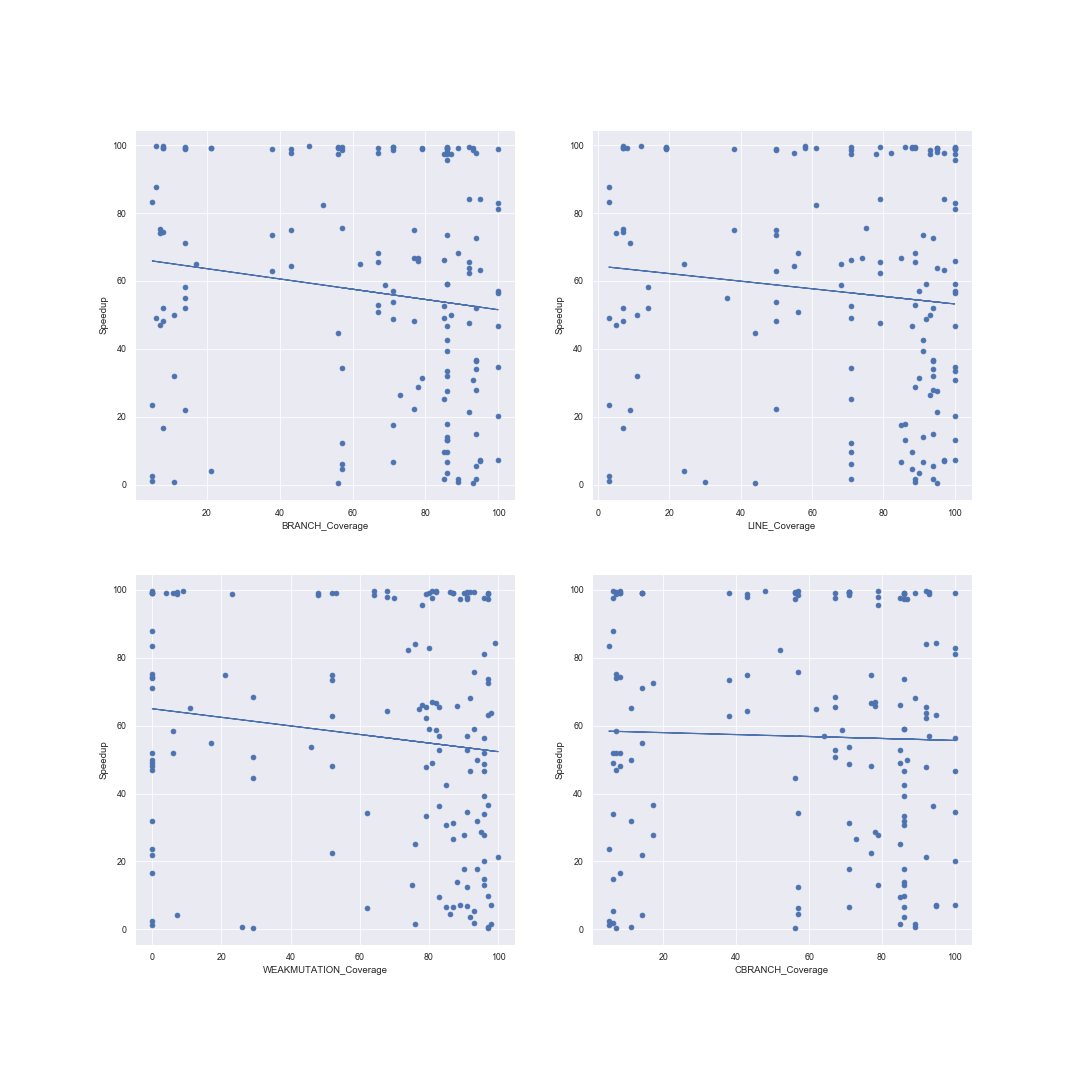
\includegraphics[width=0.8\paperwidth]{q2ScatterCorrectSpeedup.png}}
    \caption{A slight negative correlation is seen between the speedup brought by the patches and test suite coverage metrics. P values for the above lines are 0.03, 0.08, 0.09 and 0.42 for branch, line, weakmutation and cbranch coverage respectively. The exceptionally high p-value on the trend found in cbranch coverage requires additional examination to ascertain the exact relationship}
    \centering
\end{figure}

A comparison of different coverage metrics against the speedup\% observed in the evaluation tests revealed a slightly positive correlation. Using all sampled tests at 100\%, 75\%, 50\% and 25\%, we found the subset of all 528 patches produced by the test suites which did not overfit to the training test suites. The performance of these patches were then represented as data points and plotted against the coverage metrics of the test suites used to generate them. In doing so, we hoped to find correlations between the coverage metrics and the performance increase in the tests. Linear regression was then used to produce a regression-line for the given data. The results of this are shown in Figure 7. 

Another obstacle in obtaining patches with high increases in performance is the CPU clock speed. The typical runtime of the evaluation test is $10^7$ nanoseconds. This means that measuring performance improvement of 1\% requires an accuracy of $10^5$ nanoseconds. Due to the noise from variability in runtime of each run, as well as errors in measurement by the CPU clock, performance improvements in runtime are difficult to measure accurately. Thus, some mutations might be caused by random error in the calculation of the actual runtime of the patched source code. This source of noise results in the unusually high p-values obtained.

Figure 7 shows that with the exception of conditional branch coverage, there is a positive correlation between coverage and the performance of the patches.This can also be explained by the similarity between the training test suites and the evaluation suite. As coverage of the training suite improves, the search process is increasingly limited, as new patches are evaluated on a more stringent set of test cases. However, patches trained to find improvements on a training test suite with high line coverage might also find strong performance improvements on another test suite with high line coverage. Of course, this also varies depending on the context. Conversely, on an evaluation suite with low conditional-branch coverage, conditional-branch coverage on the training test suite might provide an unnecessary hindrance to the improvement process. By restricting the movement of the patch in the improvement process, unnecessary restriction of test suite metrics might result in a weaker patch produced. This begs the question - at which point does an increase in coverage result in negative impacts on the optimisations found? While our results support the idea that such a point exists between the training test suite and the evaluation suite,  more work is needed to obtain a conclusive answer. Another question which needs to be asked is of how many of these patches present universal optimisations, instead of optimisations for just the evaluation suite? While we believe that improvement in the evaluation suite is sufficient evidence that the patch generalises, perhaps a more comprehensive study can be conducted to understand the extent to which this is true.\\

\subsubsection{An overview of results so far: Test suite generation criterion and coverage metrics}
Through the first and second study, we obtained evidence that both test suite generation criteria and test suite coverage metrics indeed have a significant impact on the patches generated by the GI process.  We were able to observe trends between test suite generation criteria and the correctness and speedup of the patches generated. In particular, Test suites optimised for branch coverage performed relatively well against test suites optimised for other forms of coverage, producing patches which overfit the least frequently, as well as patches which brought higher levels of speedup in the program. This result may be used to affect our choice of coverage criteria in generated tests as input to the GI process. 

These results corroborate findings obtained in experiments on program repair. Jooyong Yi et al \cite{yicorrelation} show that there is a negative correlation between traditional test suite coverage metrics and overfitting. Other experiments by Smith et al \cite{cure} also show similar results in the use of GI for program repair. Indeed, the coverage of the provided test suite does seem to have a significant impact on the GI process for program repair. This can be attributed to 2 factors. Firstly, both non-functional improvement and program repair relies on the provided test suite as a measure of functional correctness. While in our study, the context of non-functional improvement means that programs start in a state assumed to already be ‘correct’, and the test-suite generated merely serves as a guide to reduce the search space of improvements, higher coverage of test suites still provides increased assurance about the effectiveness of the test suite in ensuring required functional behaviour is not broken. However automated testing might fail to consider some characteristics of the program, \cite{coveragecombination}. While an increase in coverage of developer written tests typically means that more functionality of the code is tested, an increase in coverage of automated test suites might not lead to a stronger test. That being said, coverage is one measurable aspect of test suites which we can look to optimise to achieve a better test suite in general.

Our experiment also highlighted another finding - many improvements found through the GI process might be contextual, and specialised based on the evaluation suite. In terms of overfitting, patches generated using automated test suites which shared similar characteristics with the evaluation test suite appeared to overfit less to the training test suite. In reality, it might simply be that these patches were coincidentally well-fitted to the evaluation suite as well. The same idea might hold for improvements in runtime.  While it is probable that many of these optimisations are universal and generalise sufficiently, more work is needed to examine the idea that these patches might just provide optimisations specialised to the training and evaluation suite. A useful outcome from this is that we can design the test suite provided to be as close as possible to the application patterns of the actual software. 


\subsection{How do automated test suites compare against user-written test-suites as inputs to the GI Process?}

Given that we have shown that automated test suites can produce quality patches capable of improving non-functional properties of a program. We now want to find out how automated test suites compare against manual tests as input to the Genetic improvement process, and how much better or worse they are at generating good patches. To answer this question, we compared automatic and manual test suites based on 2 criteria.

The first criteria is the test suites’ ability to produce non-overfitting patches. While overfitting to the training test suite to some extent is expected in the GI process, we wanted to see if using manual or automatically generated test suites provided any significant advantage in this area. For fairness, patches generated by automated  test suites were evaluated using a manually written test suite written by humans, while the patches generated by manual test suites were assessed against an automatically generated test suite, optimised for all 4 coverage metrics. Out of 381 patches generated from automated tests and 40 patches from their manual counterparts, we conducted a comparison between these 2 groups of patches and their overfitting rate. 
\begin{figure}
    \begin{center}
        \resizebox{0.8\textwidth}{!}{\input{q3BarManualvsAutoCorrectness.pgf}}
    \end{center}
    \caption{Patches generated using manual test suites overfit much less than those generated using automated test suites}
\end{figure}

Figure 8 shows the number of non-overfitting and overfitting patches generated, grouped by their provenance (automated or manually written). Similar to our first research question, overfitting here refers to both functional overfitting and non-functional overfitting, where the patches degraded performance of the program on the evaluation suite substantially. Here, we see that manual test suites still outperform automated test suites by far, generating overfitting patches only 6 out of 40 times. On the other hand, EvoSuite generated overfitting patches 283 times out of 381. This result confirms what we already know - developer written test suites are more likely to encapsulate and thus specify the behaviour of the program. They thus serve as much stronger test suites. While automated test suites are rapidly improving \cite{evosuitecompetition}, they are still not able to replicate the performance of manually written patches. One caveat to this is that our experiment only used test suites which optimised for a single coverage criterion. The use of automated test suites optimised for more than one coverage criterion might possibly lead to stronger tests, but are still unlikely to trump manual testing for now. \\

The second criteria is the test suites’ ability to generate quality patches which could improve the runtime of the program. Using the same dataset, we grouped the test suites by their provenance and used the data to create a boxplot of all patches generated. These boxplots show the median, upper and lower quartiles of the distribution and upper and lower limits.



\begin{figure}
    \begin{center}
        \resizebox{0.8\textwidth}{!}{%% Creator: Matplotlib, PGF backend
%%
%% To include the figure in your LaTeX document, write
%%   \input{<filename>.pgf}
%%
%% Make sure the required packages are loaded in your preamble
%%   \usepackage{pgf}
%%
%% Figures using additional raster images can only be included by \input if
%% they are in the same directory as the main LaTeX file. For loading figures
%% from other directories you can use the `import` package
%%   \usepackage{import}
%% and then include the figures with
%%   \import{<path to file>}{<filename>.pgf}
%%
%% Matplotlib used the following preamble
%%
\begingroup%
\makeatletter%
\begin{pgfpicture}%
\pgfpathrectangle{\pgfpointorigin}{\pgfqpoint{6.000000in}{4.000000in}}%
\pgfusepath{use as bounding box, clip}%
\begin{pgfscope}%
\pgfsetbuttcap%
\pgfsetmiterjoin%
\definecolor{currentfill}{rgb}{1.000000,1.000000,1.000000}%
\pgfsetfillcolor{currentfill}%
\pgfsetlinewidth{0.000000pt}%
\definecolor{currentstroke}{rgb}{1.000000,1.000000,1.000000}%
\pgfsetstrokecolor{currentstroke}%
\pgfsetdash{}{0pt}%
\pgfpathmoveto{\pgfqpoint{0.000000in}{0.000000in}}%
\pgfpathlineto{\pgfqpoint{6.000000in}{0.000000in}}%
\pgfpathlineto{\pgfqpoint{6.000000in}{4.000000in}}%
\pgfpathlineto{\pgfqpoint{0.000000in}{4.000000in}}%
\pgfpathclose%
\pgfusepath{fill}%
\end{pgfscope}%
\begin{pgfscope}%
\pgfsetbuttcap%
\pgfsetmiterjoin%
\definecolor{currentfill}{rgb}{0.917647,0.917647,0.949020}%
\pgfsetfillcolor{currentfill}%
\pgfsetlinewidth{0.000000pt}%
\definecolor{currentstroke}{rgb}{0.000000,0.000000,0.000000}%
\pgfsetstrokecolor{currentstroke}%
\pgfsetstrokeopacity{0.000000}%
\pgfsetdash{}{0pt}%
\pgfpathmoveto{\pgfqpoint{0.750000in}{0.500000in}}%
\pgfpathlineto{\pgfqpoint{5.400000in}{0.500000in}}%
\pgfpathlineto{\pgfqpoint{5.400000in}{3.520000in}}%
\pgfpathlineto{\pgfqpoint{0.750000in}{3.520000in}}%
\pgfpathclose%
\pgfusepath{fill}%
\end{pgfscope}%
\begin{pgfscope}%
\pgfpathrectangle{\pgfqpoint{0.750000in}{0.500000in}}{\pgfqpoint{4.650000in}{3.020000in}}%
\pgfusepath{clip}%
\pgfsetroundcap%
\pgfsetroundjoin%
\pgfsetlinewidth{0.803000pt}%
\definecolor{currentstroke}{rgb}{1.000000,1.000000,1.000000}%
\pgfsetstrokecolor{currentstroke}%
\pgfsetdash{}{0pt}%
\pgfpathmoveto{\pgfqpoint{1.912500in}{0.500000in}}%
\pgfpathlineto{\pgfqpoint{1.912500in}{3.520000in}}%
\pgfusepath{stroke}%
\end{pgfscope}%
\begin{pgfscope}%
\definecolor{textcolor}{rgb}{0.150000,0.150000,0.150000}%
\pgfsetstrokecolor{textcolor}%
\pgfsetfillcolor{textcolor}%
\pgftext[x=1.912500in,y=0.384722in,,top]{\color{textcolor}\rmfamily\fontsize{12.500000}{15.000000}\selectfont Automated Test Suites}%
\end{pgfscope}%
\begin{pgfscope}%
\pgfpathrectangle{\pgfqpoint{0.750000in}{0.500000in}}{\pgfqpoint{4.650000in}{3.020000in}}%
\pgfusepath{clip}%
\pgfsetroundcap%
\pgfsetroundjoin%
\pgfsetlinewidth{0.803000pt}%
\definecolor{currentstroke}{rgb}{1.000000,1.000000,1.000000}%
\pgfsetstrokecolor{currentstroke}%
\pgfsetdash{}{0pt}%
\pgfpathmoveto{\pgfqpoint{4.237500in}{0.500000in}}%
\pgfpathlineto{\pgfqpoint{4.237500in}{3.520000in}}%
\pgfusepath{stroke}%
\end{pgfscope}%
\begin{pgfscope}%
\definecolor{textcolor}{rgb}{0.150000,0.150000,0.150000}%
\pgfsetstrokecolor{textcolor}%
\pgfsetfillcolor{textcolor}%
\pgftext[x=4.237500in,y=0.384722in,,top]{\color{textcolor}\rmfamily\fontsize{12.500000}{15.000000}\selectfont Manual Test Suites}%
\end{pgfscope}%
\begin{pgfscope}%
\pgfpathrectangle{\pgfqpoint{0.750000in}{0.500000in}}{\pgfqpoint{4.650000in}{3.020000in}}%
\pgfusepath{clip}%
\pgfsetroundcap%
\pgfsetroundjoin%
\pgfsetlinewidth{0.803000pt}%
\definecolor{currentstroke}{rgb}{1.000000,1.000000,1.000000}%
\pgfsetstrokecolor{currentstroke}%
\pgfsetdash{}{0pt}%
\pgfpathmoveto{\pgfqpoint{0.750000in}{0.870330in}}%
\pgfpathlineto{\pgfqpoint{5.400000in}{0.870330in}}%
\pgfusepath{stroke}%
\end{pgfscope}%
\begin{pgfscope}%
\definecolor{textcolor}{rgb}{0.150000,0.150000,0.150000}%
\pgfsetstrokecolor{textcolor}%
\pgfsetfillcolor{textcolor}%
\pgftext[x=0.553126in,y=0.812460in,left,base]{\color{textcolor}\rmfamily\fontsize{12.500000}{15.000000}\selectfont \(\displaystyle 0\)}%
\end{pgfscope}%
\begin{pgfscope}%
\pgfpathrectangle{\pgfqpoint{0.750000in}{0.500000in}}{\pgfqpoint{4.650000in}{3.020000in}}%
\pgfusepath{clip}%
\pgfsetroundcap%
\pgfsetroundjoin%
\pgfsetlinewidth{0.803000pt}%
\definecolor{currentstroke}{rgb}{1.000000,1.000000,1.000000}%
\pgfsetstrokecolor{currentstroke}%
\pgfsetdash{}{0pt}%
\pgfpathmoveto{\pgfqpoint{0.750000in}{1.378226in}}%
\pgfpathlineto{\pgfqpoint{5.400000in}{1.378226in}}%
\pgfusepath{stroke}%
\end{pgfscope}%
\begin{pgfscope}%
\definecolor{textcolor}{rgb}{0.150000,0.150000,0.150000}%
\pgfsetstrokecolor{textcolor}%
\pgfsetfillcolor{textcolor}%
\pgftext[x=0.471529in,y=1.320355in,left,base]{\color{textcolor}\rmfamily\fontsize{12.500000}{15.000000}\selectfont \(\displaystyle 20\)}%
\end{pgfscope}%
\begin{pgfscope}%
\pgfpathrectangle{\pgfqpoint{0.750000in}{0.500000in}}{\pgfqpoint{4.650000in}{3.020000in}}%
\pgfusepath{clip}%
\pgfsetroundcap%
\pgfsetroundjoin%
\pgfsetlinewidth{0.803000pt}%
\definecolor{currentstroke}{rgb}{1.000000,1.000000,1.000000}%
\pgfsetstrokecolor{currentstroke}%
\pgfsetdash{}{0pt}%
\pgfpathmoveto{\pgfqpoint{0.750000in}{1.886121in}}%
\pgfpathlineto{\pgfqpoint{5.400000in}{1.886121in}}%
\pgfusepath{stroke}%
\end{pgfscope}%
\begin{pgfscope}%
\definecolor{textcolor}{rgb}{0.150000,0.150000,0.150000}%
\pgfsetstrokecolor{textcolor}%
\pgfsetfillcolor{textcolor}%
\pgftext[x=0.471529in,y=1.828251in,left,base]{\color{textcolor}\rmfamily\fontsize{12.500000}{15.000000}\selectfont \(\displaystyle 40\)}%
\end{pgfscope}%
\begin{pgfscope}%
\pgfpathrectangle{\pgfqpoint{0.750000in}{0.500000in}}{\pgfqpoint{4.650000in}{3.020000in}}%
\pgfusepath{clip}%
\pgfsetroundcap%
\pgfsetroundjoin%
\pgfsetlinewidth{0.803000pt}%
\definecolor{currentstroke}{rgb}{1.000000,1.000000,1.000000}%
\pgfsetstrokecolor{currentstroke}%
\pgfsetdash{}{0pt}%
\pgfpathmoveto{\pgfqpoint{0.750000in}{2.394017in}}%
\pgfpathlineto{\pgfqpoint{5.400000in}{2.394017in}}%
\pgfusepath{stroke}%
\end{pgfscope}%
\begin{pgfscope}%
\definecolor{textcolor}{rgb}{0.150000,0.150000,0.150000}%
\pgfsetstrokecolor{textcolor}%
\pgfsetfillcolor{textcolor}%
\pgftext[x=0.471529in,y=2.336147in,left,base]{\color{textcolor}\rmfamily\fontsize{12.500000}{15.000000}\selectfont \(\displaystyle 60\)}%
\end{pgfscope}%
\begin{pgfscope}%
\pgfpathrectangle{\pgfqpoint{0.750000in}{0.500000in}}{\pgfqpoint{4.650000in}{3.020000in}}%
\pgfusepath{clip}%
\pgfsetroundcap%
\pgfsetroundjoin%
\pgfsetlinewidth{0.803000pt}%
\definecolor{currentstroke}{rgb}{1.000000,1.000000,1.000000}%
\pgfsetstrokecolor{currentstroke}%
\pgfsetdash{}{0pt}%
\pgfpathmoveto{\pgfqpoint{0.750000in}{2.901912in}}%
\pgfpathlineto{\pgfqpoint{5.400000in}{2.901912in}}%
\pgfusepath{stroke}%
\end{pgfscope}%
\begin{pgfscope}%
\definecolor{textcolor}{rgb}{0.150000,0.150000,0.150000}%
\pgfsetstrokecolor{textcolor}%
\pgfsetfillcolor{textcolor}%
\pgftext[x=0.471529in,y=2.844042in,left,base]{\color{textcolor}\rmfamily\fontsize{12.500000}{15.000000}\selectfont \(\displaystyle 80\)}%
\end{pgfscope}%
\begin{pgfscope}%
\pgfpathrectangle{\pgfqpoint{0.750000in}{0.500000in}}{\pgfqpoint{4.650000in}{3.020000in}}%
\pgfusepath{clip}%
\pgfsetroundcap%
\pgfsetroundjoin%
\pgfsetlinewidth{0.803000pt}%
\definecolor{currentstroke}{rgb}{1.000000,1.000000,1.000000}%
\pgfsetstrokecolor{currentstroke}%
\pgfsetdash{}{0pt}%
\pgfpathmoveto{\pgfqpoint{0.750000in}{3.409808in}}%
\pgfpathlineto{\pgfqpoint{5.400000in}{3.409808in}}%
\pgfusepath{stroke}%
\end{pgfscope}%
\begin{pgfscope}%
\definecolor{textcolor}{rgb}{0.150000,0.150000,0.150000}%
\pgfsetstrokecolor{textcolor}%
\pgfsetfillcolor{textcolor}%
\pgftext[x=0.389933in,y=3.351938in,left,base]{\color{textcolor}\rmfamily\fontsize{12.500000}{15.000000}\selectfont \(\displaystyle 100\)}%
\end{pgfscope}%
\begin{pgfscope}%
\definecolor{textcolor}{rgb}{0.150000,0.150000,0.150000}%
\pgfsetstrokecolor{textcolor}%
\pgfsetfillcolor{textcolor}%
\pgftext[x=0.334378in,y=2.010000in,,bottom,rotate=90.000000]{\color{textcolor}\rmfamily\fontsize{13.000000}{15.600000}\selectfont \% Speedup on evaluation test}%
\end{pgfscope}%
\begin{pgfscope}%
\pgfpathrectangle{\pgfqpoint{0.750000in}{0.500000in}}{\pgfqpoint{4.650000in}{3.020000in}}%
\pgfusepath{clip}%
\pgfsetroundcap%
\pgfsetroundjoin%
\pgfsetlinewidth{1.003750pt}%
\definecolor{currentstroke}{rgb}{0.000000,0.000000,0.000000}%
\pgfsetstrokecolor{currentstroke}%
\pgfsetdash{}{0pt}%
\pgfpathmoveto{\pgfqpoint{1.738125in}{0.876448in}}%
\pgfpathlineto{\pgfqpoint{2.086875in}{0.876448in}}%
\pgfpathlineto{\pgfqpoint{2.086875in}{1.982504in}}%
\pgfpathlineto{\pgfqpoint{1.738125in}{1.982504in}}%
\pgfpathlineto{\pgfqpoint{1.738125in}{0.876448in}}%
\pgfusepath{stroke}%
\end{pgfscope}%
\begin{pgfscope}%
\pgfpathrectangle{\pgfqpoint{0.750000in}{0.500000in}}{\pgfqpoint{4.650000in}{3.020000in}}%
\pgfusepath{clip}%
\pgfsetroundcap%
\pgfsetroundjoin%
\pgfsetlinewidth{1.003750pt}%
\definecolor{currentstroke}{rgb}{0.000000,0.000000,0.000000}%
\pgfsetstrokecolor{currentstroke}%
\pgfsetdash{}{0pt}%
\pgfpathmoveto{\pgfqpoint{1.912500in}{0.876448in}}%
\pgfpathlineto{\pgfqpoint{1.912500in}{0.637273in}}%
\pgfusepath{stroke}%
\end{pgfscope}%
\begin{pgfscope}%
\pgfpathrectangle{\pgfqpoint{0.750000in}{0.500000in}}{\pgfqpoint{4.650000in}{3.020000in}}%
\pgfusepath{clip}%
\pgfsetroundcap%
\pgfsetroundjoin%
\pgfsetlinewidth{1.003750pt}%
\definecolor{currentstroke}{rgb}{0.000000,0.000000,0.000000}%
\pgfsetstrokecolor{currentstroke}%
\pgfsetdash{}{0pt}%
\pgfpathmoveto{\pgfqpoint{1.912500in}{1.982504in}}%
\pgfpathlineto{\pgfqpoint{1.912500in}{3.382727in}}%
\pgfusepath{stroke}%
\end{pgfscope}%
\begin{pgfscope}%
\pgfpathrectangle{\pgfqpoint{0.750000in}{0.500000in}}{\pgfqpoint{4.650000in}{3.020000in}}%
\pgfusepath{clip}%
\pgfsetroundcap%
\pgfsetroundjoin%
\pgfsetlinewidth{1.003750pt}%
\definecolor{currentstroke}{rgb}{0.000000,0.000000,0.000000}%
\pgfsetstrokecolor{currentstroke}%
\pgfsetdash{}{0pt}%
\pgfpathmoveto{\pgfqpoint{1.825313in}{0.637273in}}%
\pgfpathlineto{\pgfqpoint{1.999688in}{0.637273in}}%
\pgfusepath{stroke}%
\end{pgfscope}%
\begin{pgfscope}%
\pgfpathrectangle{\pgfqpoint{0.750000in}{0.500000in}}{\pgfqpoint{4.650000in}{3.020000in}}%
\pgfusepath{clip}%
\pgfsetroundcap%
\pgfsetroundjoin%
\pgfsetlinewidth{1.003750pt}%
\definecolor{currentstroke}{rgb}{0.000000,0.000000,0.000000}%
\pgfsetstrokecolor{currentstroke}%
\pgfsetdash{}{0pt}%
\pgfpathmoveto{\pgfqpoint{1.825313in}{3.382727in}}%
\pgfpathlineto{\pgfqpoint{1.999688in}{3.382727in}}%
\pgfusepath{stroke}%
\end{pgfscope}%
\begin{pgfscope}%
\pgfpathrectangle{\pgfqpoint{0.750000in}{0.500000in}}{\pgfqpoint{4.650000in}{3.020000in}}%
\pgfusepath{clip}%
\pgfsetroundcap%
\pgfsetroundjoin%
\pgfsetlinewidth{1.003750pt}%
\definecolor{currentstroke}{rgb}{0.000000,0.000000,0.000000}%
\pgfsetstrokecolor{currentstroke}%
\pgfsetdash{}{0pt}%
\pgfpathmoveto{\pgfqpoint{4.063125in}{0.821635in}}%
\pgfpathlineto{\pgfqpoint{4.411875in}{0.821635in}}%
\pgfpathlineto{\pgfqpoint{4.411875in}{0.992468in}}%
\pgfpathlineto{\pgfqpoint{4.063125in}{0.992468in}}%
\pgfpathlineto{\pgfqpoint{4.063125in}{0.821635in}}%
\pgfusepath{stroke}%
\end{pgfscope}%
\begin{pgfscope}%
\pgfpathrectangle{\pgfqpoint{0.750000in}{0.500000in}}{\pgfqpoint{4.650000in}{3.020000in}}%
\pgfusepath{clip}%
\pgfsetroundcap%
\pgfsetroundjoin%
\pgfsetlinewidth{1.003750pt}%
\definecolor{currentstroke}{rgb}{0.000000,0.000000,0.000000}%
\pgfsetstrokecolor{currentstroke}%
\pgfsetdash{}{0pt}%
\pgfpathmoveto{\pgfqpoint{4.237500in}{0.821635in}}%
\pgfpathlineto{\pgfqpoint{4.237500in}{0.638963in}}%
\pgfusepath{stroke}%
\end{pgfscope}%
\begin{pgfscope}%
\pgfpathrectangle{\pgfqpoint{0.750000in}{0.500000in}}{\pgfqpoint{4.650000in}{3.020000in}}%
\pgfusepath{clip}%
\pgfsetroundcap%
\pgfsetroundjoin%
\pgfsetlinewidth{1.003750pt}%
\definecolor{currentstroke}{rgb}{0.000000,0.000000,0.000000}%
\pgfsetstrokecolor{currentstroke}%
\pgfsetdash{}{0pt}%
\pgfpathmoveto{\pgfqpoint{4.237500in}{0.992468in}}%
\pgfpathlineto{\pgfqpoint{4.237500in}{1.219831in}}%
\pgfusepath{stroke}%
\end{pgfscope}%
\begin{pgfscope}%
\pgfpathrectangle{\pgfqpoint{0.750000in}{0.500000in}}{\pgfqpoint{4.650000in}{3.020000in}}%
\pgfusepath{clip}%
\pgfsetroundcap%
\pgfsetroundjoin%
\pgfsetlinewidth{1.003750pt}%
\definecolor{currentstroke}{rgb}{0.000000,0.000000,0.000000}%
\pgfsetstrokecolor{currentstroke}%
\pgfsetdash{}{0pt}%
\pgfpathmoveto{\pgfqpoint{4.150313in}{0.638963in}}%
\pgfpathlineto{\pgfqpoint{4.324688in}{0.638963in}}%
\pgfusepath{stroke}%
\end{pgfscope}%
\begin{pgfscope}%
\pgfpathrectangle{\pgfqpoint{0.750000in}{0.500000in}}{\pgfqpoint{4.650000in}{3.020000in}}%
\pgfusepath{clip}%
\pgfsetroundcap%
\pgfsetroundjoin%
\pgfsetlinewidth{1.003750pt}%
\definecolor{currentstroke}{rgb}{0.000000,0.000000,0.000000}%
\pgfsetstrokecolor{currentstroke}%
\pgfsetdash{}{0pt}%
\pgfpathmoveto{\pgfqpoint{4.150313in}{1.219831in}}%
\pgfpathlineto{\pgfqpoint{4.324688in}{1.219831in}}%
\pgfusepath{stroke}%
\end{pgfscope}%
\begin{pgfscope}%
\pgfpathrectangle{\pgfqpoint{0.750000in}{0.500000in}}{\pgfqpoint{4.650000in}{3.020000in}}%
\pgfusepath{clip}%
\pgfsetroundcap%
\pgfsetroundjoin%
\pgfsetlinewidth{1.003750pt}%
\definecolor{currentstroke}{rgb}{0.866667,0.517647,0.321569}%
\pgfsetstrokecolor{currentstroke}%
\pgfsetdash{}{0pt}%
\pgfpathmoveto{\pgfqpoint{1.738125in}{1.166914in}}%
\pgfpathlineto{\pgfqpoint{2.086875in}{1.166914in}}%
\pgfusepath{stroke}%
\end{pgfscope}%
\begin{pgfscope}%
\pgfpathrectangle{\pgfqpoint{0.750000in}{0.500000in}}{\pgfqpoint{4.650000in}{3.020000in}}%
\pgfusepath{clip}%
\pgfsetroundcap%
\pgfsetroundjoin%
\pgfsetlinewidth{1.003750pt}%
\definecolor{currentstroke}{rgb}{0.866667,0.517647,0.321569}%
\pgfsetstrokecolor{currentstroke}%
\pgfsetdash{}{0pt}%
\pgfpathmoveto{\pgfqpoint{4.063125in}{0.885379in}}%
\pgfpathlineto{\pgfqpoint{4.411875in}{0.885379in}}%
\pgfusepath{stroke}%
\end{pgfscope}%
\begin{pgfscope}%
\pgfsetrectcap%
\pgfsetmiterjoin%
\pgfsetlinewidth{1.003750pt}%
\definecolor{currentstroke}{rgb}{1.000000,1.000000,1.000000}%
\pgfsetstrokecolor{currentstroke}%
\pgfsetdash{}{0pt}%
\pgfpathmoveto{\pgfqpoint{0.750000in}{0.500000in}}%
\pgfpathlineto{\pgfqpoint{0.750000in}{3.520000in}}%
\pgfusepath{stroke}%
\end{pgfscope}%
\begin{pgfscope}%
\pgfsetrectcap%
\pgfsetmiterjoin%
\pgfsetlinewidth{1.003750pt}%
\definecolor{currentstroke}{rgb}{1.000000,1.000000,1.000000}%
\pgfsetstrokecolor{currentstroke}%
\pgfsetdash{}{0pt}%
\pgfpathmoveto{\pgfqpoint{5.400000in}{0.500000in}}%
\pgfpathlineto{\pgfqpoint{5.400000in}{3.520000in}}%
\pgfusepath{stroke}%
\end{pgfscope}%
\begin{pgfscope}%
\pgfsetrectcap%
\pgfsetmiterjoin%
\pgfsetlinewidth{1.003750pt}%
\definecolor{currentstroke}{rgb}{1.000000,1.000000,1.000000}%
\pgfsetstrokecolor{currentstroke}%
\pgfsetdash{}{0pt}%
\pgfpathmoveto{\pgfqpoint{0.750000in}{0.500000in}}%
\pgfpathlineto{\pgfqpoint{5.400000in}{0.500000in}}%
\pgfusepath{stroke}%
\end{pgfscope}%
\begin{pgfscope}%
\pgfsetrectcap%
\pgfsetmiterjoin%
\pgfsetlinewidth{1.003750pt}%
\definecolor{currentstroke}{rgb}{1.000000,1.000000,1.000000}%
\pgfsetstrokecolor{currentstroke}%
\pgfsetdash{}{0pt}%
\pgfpathmoveto{\pgfqpoint{0.750000in}{3.520000in}}%
\pgfpathlineto{\pgfqpoint{5.400000in}{3.520000in}}%
\pgfusepath{stroke}%
\end{pgfscope}%
\end{pgfpicture}%
\makeatother%
\endgroup%
}
    \end{center}
    \caption{Patches from automatically generated tests showed a significantly higher increase in performance than those generated from manual test suites. These results have a p-value of 0.0003, which show that there is sufficient evidence to support our conclusion that automated test suites produce patches which produce a higher increase in performance. }
\end{figure}

Figure 9 shows a boxplot which compares the performance gains of programs patched with patches generated using automatically generated test suites as input to Gin, as well as those patched with manually written test suites as input to Gin. The boxplot shows that automatically generated test suites boast a significant advantage in producing patches which provide a larger speedup\%. As a whole, automated test suites provide a mean of 26\% speedup with a standard deviation of 33\%, while manual test suites provide only an average of 3\% improvement, albeit with a much lower standard deviation at 13\%.This provides evidence that automatically generated test suites could be more effective in finding better patches than manually written test suites. One reason for this could be that automatically generated test suites are not as restrictive as manual test suites. This means that during the evolution process, the patches are allowed to mutate in more ways, which allow them to find solutions which lead to higher increases in speed, at the cost of correctness. Thus, those patches which managed to pass the evaluation suite eventually show a higher increase in speedup\%. 

Another notable point is that the coverage of the manual test suites here were lower than that of the automated test suites. Taking an aggregated coverage value across all 4 coverage criteria collected, we see that the average coverage of the manual test suites is 88\% compared to 91\% for automated test suites. Despite this difference in coverage, the manual test suites still generate patches which overfit much less than the automated test suites. Literature on automated test suites point to the fact that automatically generated unit tests are not as effective in finding faults as manually written ones \cite{evosuitefaults}.  Other studies by Holmes et al \cite{coveragenotcorrelated} argue that traditional coverage metrics are not an accurate way of measuring the effectiveness of a test suite. Despite the high coverage values of our generated automated tests, perhaps we should look to other less- conventional metrics to determine the effectiveness of a test suite in the context of genetic improvement. \\

\begin{table}[h]
\centering
\resizebox{\textwidth}{!}{%
\begin{tabular}{l | l | l | l | l | l | l | l | l | l}
         & Count & Avg Speedup & Std & Overfit Rate & Branch & Line  & Weakmutation & C-Branch & Avg Coverage \\
EvoSuite & 98.0        & 25.57        & 33.30  & 0.74             & 93.61  & 94.01 & 90.59        & 85.56    & 90.94        \\
Manual   & 34.0        & 3.449        & 13.42  & 0.15             & 89.53  & 89.32 & 95.68        & 79.29    & 88.46       
\end{tabular}%
}
\caption{Head to head comparision between automated and manual tests used in the study. Taking the mean of all 4 coverage metrics, we see that manual tests had slightly lower average coverage at 88\% compared to that of EvoSuite-generated tests at 90\%. Despite this manual test, suites still managed to produce patches which overfit far less often}
\label{tab:table3}
\end{table}

The data obtained indicates that automatically generated test suites provide some upsides when used as inputs to the GI process. Due to the less restrictive nature of automatically generated tests, the GI process is able to spawn more mutations of the original source code which allows it to cover the search space more freely. This leads to higher quality patches when these patches do pass the evaluation suite. On the other hand, this leads to some tradeoffs. The decrease in the strength of the tests also means that a larger proportion of the automated tests fail to pass the evaluation suite. This means that a larger proportion of the generated tests overfit to the training suite. 

An implication of these results is that a two-layered approach could be used for the genetic improvement process. During the mutation process, the automated test suite can be used as a loose guide to inform the mutation process. Once patches are generated, they can be checked against the manually written evaluation suite to ensure that they still retain all functional properties. This two layered approach could allow us to reap the benefits automated test suites provide - a significant reduction in the search space, while still allowing for freedom of improvement, while maintaining the functional properties specified in the manual tests suite.



\section{Threats to Validity}
\begin{enumerate}
	\item Small Sample size \\
Due to the time and computational power needed to run the GI process, we were limited by the timeframe of our project as well as the computing resources available to us. As such, we could only run our experiments on the small number of test programs in the LocoGP benchmark set, generating 2 test suites per test. This limited the sample size of our project. In our setup, we only managed to procure one manual test suite per program, for a total of 11 programs. This meant that the strength of the manual test suites in this experiment were highly reliant on the quality of each and every manual test suite provided. Given that developers’ skills and practices vary greatly from person to person, these manual test suites might not have been representative of all manual test suites. Despite this, the programs and test suites provided in the LocoGP benchmark set has been used to benchmark various other experiments around GI \cite{locogp}. This allows our results to be directly and easily compared across other studies. The small programs chosen were sufficiently general and present a class of commonly used algorithms in computing (sorting algorithms). Moreover, we managed to generate a large enough dataset to mitigate the small sample size. 

	\item Small tests, research limited to Gin and Evosuite\\
Since our experiments were centered around Gin and subsequently EvoSuite, it might not generalise to all Genetic Improvement tools and Automated test generation tools. EvoSuite’s approach to test generation might not be replicated by other automated test generation tools. It might be the case that the similarities between the programs might reveal some sort of bias when generating patches using Gin and test cases using EvoSuite. That being said, EvoSuite is currently one of the most widely used test generation tools and the winner of multiple Search-Based Software Testing Competitions \cite{evosuitecompetition}.

	\item Low search budget for Gin \\
The search space for patches in Gin is extremely large, especially with Statement coverage used, due to the different levels of abstraction available in an AST. Despite this, we limited the number of iterations Gin made to 100 per run. This small search budget might have hindered otherwise strong test suites from generating better patches, given a larger search budget to allow Gin to traverse the search space. This could overcome the speed limitations of manual patches, but might cause further overfitting in automated test suites with less stringent test cases. Despite these limitations in compute and time, 100 generations is typically a good indicator for allowing Gin to find small optimisations. Since the programs used in our experiment were all small programs, the search space for improvements is reduced, and 100 generations should be more than sufficient to find differences.

	\item Search Strategy \\
In our experiment, we used LocalSearch as our search strategy for the GI process. The use of other search strategies such as Genetic programming and tabu search could lead to different results. 

	\item Runtime \\
As mentioned above, the limitations of the CPU clock’s accuracy make determining the exact runtime of a program hard to measure. Since runtime improvements are in the magnitude of $10^5$ nanoseconds, using the CPU clock to assess the improvements in runtime might not yield accurate results, generating noise in the data. We mitigated this  problem by conducting 10 repeated runs of the evaluation test and then taking the average runtime of these runs as an estimate of the actual runtime of the patched program. This reduces the random error, and increases the accuracy of our estimation. We also made all efforts to switch off all running background processes during the conduct of the experiment to minimise experimental noise.

\end{enumerate}
\section{Conclusions and Future Work}

Genetic Programming has seen success across many fields, in the creation and improvement of programs, as well as the improvement of various Non-functional properties of programs. In many of these fields, we have seen its efficacy in finding and repairing software bugs (cure), reduce power consumption in programs (cite bruce) and reduce memory consumption and runtime.\cite{yuewu2015}
The use of automatically generated test suites as input to the Genetic Improvement process is an exciting proposition which opens up many possibilities in software optimisation, and one which shows promise.

\subsection{Conclusion}

In this paper, we used automatic tests as inputs to the GI process and showed that it can be an effective way to develop quality patches which are able to improve the performance of programs. Patches generated with automated tests as inputs consistently show higher levels of performance gains than those generated with their manual counterparts. On the other hand, these patches suffer substantially from the overfitting problem, which needs to be addressed should the idea of using automated tests in place of manual tests be adopted, or for automated tests to be used alongside manual tests be considered. As the first study focusing on the use of automated test suites in non-functional improvement tasks, this study provides a foothold into the realm of possibilities provided by this approach. However, more work is needed to be done to analyse the impact a combination of optimisation criterion might have on generated patches, on a larger range of test programs and with varying search budgets for the GI process.

In section 1 and 2, we provided the motivation for our study and laid out the existing research in the field which motivated our study through a brief survey of current literature in the field. This allowed us to obtain insights and lessons which guided our approach in this study.
In sections 3 and 4, we provided a look at the project goals as well as the tools relevant to the study. This set the foundation for the our study and how it was to be conducted.
In section 5, we detailed the modifications made to Gin and described the experimental setup we used to conduct this study to give insight into the experimental procedure. 
In section 6, we conducted an in-depth analysis of the various factors at the Test generation stage and of generated tests which influence the quality of patches generated by Gin, through the generation of a large number of patches through a smaller number of automatically generated test suites. Here we discussed the trends observed between test generation criterion, test suite coverage and overfitting and speedup in the patches obtained.
Here, we obtained some key results from our research questions: \\

\textbf{Test generation criteria has a significant impact on overfitting rates in the generated patches. Higher coverage in automated test suites lead to lower rates of overfitting in the generated patches.} 
	
We established that test suites which optimised for branch coverage produced patches which tend to overfit less than its peers while also providing higher improvements in performance than its peers. We also confirmed that an increase in coverage metrics of automated test suites generally led to lower rates of overfitting and larger performance gains on the evaluation test suites. With that being said, the exception of conditional-branch coverage shows that test suite coverage metrics cannot be taken at face value as a measure of effectiveness of the test suites - improvements on coverage metrics which are not as relevant to the actual use of the program, represented in this case by the evaluation test suite, might not reduce overfitting by as much, and might instead cause it to overfit to the training suite. We advocate for the further study of branch coverage as a point of emphasis in the test generation process, as well as the use of high-coverage test suites where automated test suites are used as input to the GI process. \\

\textbf{Automated test suite coverage has a positive correlation with runtime improvements in generated patches.} 
	
We showed that there is a relationship between test suite coverage and runtime improvements in generated patches through our correlation study. We presumed that the improvements in runtime could be due to micro-optimisations made on the training suite which were specifically relevant to the evaluation suite. Despite this, the lack of a clear understanding of this relationship prompts us to conduct further investigation into this relationship.  \\

\textbf{Using manual test suites produce overfitting patches much less frequently, but using automated test suites produce patches which provide significantly higher increases in performance.} 
	
The idea that test suite coverage was not the best indicator of the strength of a test suite was echoed in our comparison of automated and manually written test suites, where automated test suites definitively beat manual test suites in finding patches which yield larger performance improvements, but were shown to generate overfitting patches a larger proportion of the time despite having higher coverage on average. Through this results, we are made aware of the trade offs present between both modes of test suite provenance. In doing so, we also devised a potential strategy to maximise performance gains of generated patches while ensuring the functional correctness of these patches, through a 2 layered approach. By using the automated test suite during the GI process and the manual test suite as a filter for functional properties, we might be able to reap the benefits provided by both test suites. \\\\
All data and scripts used in this study are made available at the following link:\\\\
https://github.com/mingyi850/gin




\subsection{Future Work}
Looking forward, there are further questions which need to be addressed to build on our results. \\\\
\textbf{The impact of automatically generated test suites with multiple optimisation criterion}

While our research aimed to provide some intuition for the test suite generation parameters which produced the best patches on the LocoGP benchmark suite, we were unable to test for different combinations of optimisation parameters. In doing so, the study does not account for combinatorial effects of multiple optimisation parameters, which might provide a better representation of the strength of automatically generated test suites. Moreover, more criteria could be investigated. To better understand the effect automated test suites might have on the GI process, future studies can be done on  how automatically generated test suites with multiple optimisation criterion (which more realistically depicts automatically generated test suites) might have on the generated patches.\\\\
\textbf{The relationship between the test suite coverage and increases in performance}

A closer look is needed at the effect test suite coverage has on the improvement of non-functional properties in GI. While we were able to establish that a positive correlation between the 2 does exist, we need to examine the exact relationship between the 2 and the reasons for this correlation. Achieving a solid understanding of how test suite coverage affects performance benefits in generated patches and the conditions where this holds can potentially allow us to develop test suites which are better suited to the GI process. \\\\
\textbf{Generalisation of results to larger programs}

Due to the small size of the benchmarks in the study, the runtimes of programs are of an extremely small magnitude. This can pose problems for CPU clocks to accurately measure these runtimes leading to inaccuracies in the GI process or in our measurement of runtimes. Aside from this, we also want to learn if the results we obtain during this study can generalise to larger programs. Doing so, we can increase our confidence in the ability of automated tests to be viable options in the application of GI techniques to  improve larger software.




\appendix

\begin{thebibliography}{99}

\bibitem{petkesurvey}
Petke, J., Haraldsson, S. O., Harman, M., Langdon, W. B., White, D. R., \&; Woodward, J. R. (2018). Genetic Improvement of Software: A Comprehensive Survey. IEEE Transactions on Evolutionary Computation, 22(3), 415-432. doi:10.1109/tevc.2017.2693219

\bibitem{harman2012}  
Harman, M., Mansouri, S. A. \&; Zhang, Y. (2012). Search-based software engineering: A Comprehensive Analysis and Review of Trends Techniques and Applications. ACM Computing Surveys, 45(1), 1-61. doi:10.1145/2379776.2379787

\bibitem{harman2007}
Harman, M. (2007). The Current State and Future of Search Based Software Engineering. Future of Software Engineering (FOSE '07). doi:10.1109/fose.2007.29

\bibitem{bruceenergy}
Bobby R. Bruce, Justyna Petke, and Mark Harman. 2015. Reducing Energy Consumption Using Genetic Improvement. In Proceedings of the 2015 Annual Conference on Genetic and Evolutionary Computation (GECCO '15), Sara Silva (Ed.). ACM, New York, NY, USA, 1327-1334. DOI: https://doi.org/10.1145/2739480.2754752

\bibitem{langdonharman2015}
W. B. Langdon and M. Harman, "Optimizing Existing Software With Genetic Programming," in IEEE Transactions on Evolutionary Computation, vol. 19, no. 1, pp. 118-135, Feb. 2015. doi: 10.1109/TEVC.2013.2281544

\bibitem{yuewu2015}
Wu, F., Weimer, W., Harman, M., Jia, Y., \&; Krinke, J. (2015). Deep Parameter Optimisation. Proceedings of the 2015 on Genetic and Evolutionary Computation Conference - GECCO '15. doi:10.1145/2739480.2754648

\bibitem{qireiss2017}
Qi Xin and Steven P. Reiss. 2017. Identifying test-suite-overfitted patches through test case generation. In Proceedings of the 26th ACM SIGSOFT International Symposium on Software Testing and Analysis (ISSTA 2017). ACM, New York, NY, USA, 226-236. DOI: https://doi.org/10.1145/3092703.3092718

\bibitem{petkegin}
Petke, J \& Brownlee, AEI. (2019). Software Improvement with Gin: a Case Study.

\bibitem{cure}
Edward K. Smith, Earl T. Barr, Claire Le Goues, and Yuriy Brun. 2015. Is the cure worse than the disease? overfitting in automated program repair. In Proceedings of the 2015 10th Joint Meeting on Foundations of Software Engineering (ESEC/FSE 2015). ACM, New York, NY, USA, 532-543. DOI: https://doi.org/10.1145/2786805.2786825

\bibitem{genprog}
Goues, C. L., Nguyen, T., Forrest, S., \&; Weimer, W. (2012). GenProg: A Generic Method for Automatic Software Repair. IEEE Transactions on Software Engineering, 38(1), 54-72. doi:10.1109/tse.2011.104

\bibitem{petkespecialise}
Petke, J., Harman, M., Langdon, W. B., \&; Weimer, W. (2018). Specialising Software for Different Downstream Applications Using Genetic Improvement and Code Transplantation. IEEE Transactions on Software Engineering, 44(6), 574-594. doi:10.1109/tse.2017.2702606

\bibitem{fitnessfunction}
Fast, E., Gouse, C. L., Forrest, S., \&; Weimer, W. (2010). Designing better fitness functions for automated program repair. Proceedings of the 12th Annual Conference on Genetic and Evolutionary Computation - GECCO '10. doi:10.1145/1830483.1830654

\bibitem{yicorrelation}
Yi, J., Tan, S.H., Mechtaev, S. et al. Empir Software Eng (2018) A correlation study between automated program repair and test-suite metrics 23: 2948. https://doi.org/10.1007/s10664-017-9552-y

\bibitem{xiongliu2018}
Yingfei Xiong, Xinyuan Liu, Muhan Zeng, Lu Zhang, and Gang Huang. 2018. Identifying patch correctness in test-based program repair. In Proceedings of the 40th International Conference on Software Engineering (ICSE '18). ACM, New York, NY, USA, 789-799. DOI: https://doi.org/10.1145/3180155.3180182

\bibitem{yumartinez2019}
Yu, Z., Martinez, M., Danglot, B. et al. Empir Software Eng (2019) Alleviating patch overfitting with automatic test generation: a study of feasibility and effectiveness for the Nopol repair system 24: 33. https://doi.org/10.1007/s10664-018-9619-4

\bibitem{evosuitefaults}
Shamshiri, S., Just, R., Rojas, J. M., Fraser, G., Mcminn, P., \&; Arcuri, A. (2015). Do Automatically Generated Unit Tests Find Real Faults? An Empirical Study of Effectiveness and Challenges (T). 2015 30th IEEE/ACM International Conference on Automated Software Engineering (ASE). doi:10.1109/ase.2015.86

\bibitem{coveragecombination}
Gay, G. (2017). Generating Effective Test Suites by Combining Coverage Criteria. Search Based Software Engineering Lecture Notes in Computer Science, 65-82. doi:10.1007/978-3-319-66299-2\_5

\bibitem{gincasestudy}
Petke, J., \&; Brownlee, A. E. (2019). Software Improvement with Gin: A Case Study. Search-Based Software Engineering Lecture Notes in Computer Science, 183-189. doi:10.1007/978-3-030-27455-9\_14

\bibitem{plasticsurgery}
Barr, E. T., Brun, Y., Devanbu, P., Harman, M., \&; Sarro, F. (2014). The plastic surgery hypothesis. Proceedings of the 22nd ACM SIGSOFT International Symposium on Foundations of Software Engineering - FSE 2014. doi:10.1145/2635868.2635898

\bibitem{bobbyblind}
Bruce, Bobby. (2018). The Blind Software Engineer: Improving the Non-Functional Properties of Software by Means of Genetic Improvement. 

\bibitem{pyggi2}
An, G., Blot, A., Petke, J., \&; Yoo, S. (2019). PyGGI 2.0: Language independent genetic improvement framework. Proceedings of the 2019 27th ACM Joint Meeting on European Software Engineering Conference and Symposium on the Foundations of Software Engineering - ESEC/FSE 2019. doi:10.1145/3338906.3341184

\bibitem{testingtextbook}
Pezze, M., \&; Young, M. (2008). 14. In Software testing and analysis: Process, principles, and techniques (pp. 39-111). Hoboken, NJ: Wiley.

\bibitem{mutation1}
Jia, Y., \&; Harman, M. (2011). An Analysis and Survey of the Development of Mutation Testing. IEEE Transactions on Software Engineering, 37(5), 649-678. doi:10.1109/tse.2010.62

\bibitem{mutation2}
Zhu, Q., Panichella, A., \&; Zaidman, A. (2016). A systematic literature review of how mutation testing supports test activities. doi:10.7287/peerj.preprints.2483

\bibitem{strongweakmutation}
Offutt, A. J., \&; Lee, S. D. (1991). How strong is weak mutation? Proceedings of the Symposium on Testing, Analysis, and Verification - TAV4. doi:10.1145/120807.120826

\bibitem{outputdiversity}
Alshahwan, N., \&; Harman, M. (2012). Augmenting test suites effectiveness by increasing output diversity. 2012 34th International Conference on Software Engineering (ICSE). doi:10.1109/icse.2012.6227083

\bibitem{souzagouesgenprog2018}
Oliveira, V. P., Souza, E. F., Goues, C. L., \&; Camilo-Junior, C. G. (2018). Improved representation and genetic operators for linear genetic programming for automated program repair. Empirical Software Engineering, 23(5), 2980-3006. doi:10.1007/s10664-017-9562-9

\bibitem{statsmodel}
Seabold, Skipper, and Josef Perktold. “statsmodels: Econometric and statistical modeling with python.” Proceedings of the 9th Python in Science Conference. 2010.

\bibitem{gouesrepair2013}
Goues, C. L. (2013). Automatic Program Repair Using Genetic Programming. doi:10.18130/v3kz3c

\bibitem{coveragenotcorrelated}
Inozemtseva, L., \&; Holmes, R. (2014). Coverage is not strongly correlated with test suite effectiveness. Proceedings of the 36th International Conference on Software Engineering - ICSE 2014. doi:10.1145/2568225.2568271

\bibitem{evosuitecompetition}
G. Fraser and A. Arcuri, “EvoSuite at the SBST 2017 Tool Competition,” in 10th International Workshop on Search-Based Software Testing (SBST’17) at ICSE’17, 2017, pp. 39-42.

\bibitem{locogp}
Cody-Kenny, B., Galván-López, E., \&; Barrett, S. (2015). LocoGP. Proceedings of the Companion Publication of the 2015 on Genetic and Evolutionary Computation Conference - GECCO Companion '15. doi:10.1145/2739482.2768419

\end{thebibliography}
\section{Appendix}

All data and scripts needed for replication is available on the accompanying repository: \\
https://github.com/mingyi850/gin \\\\
All generated data used in this study is available at: \\
https://github.com/mingyi850/gin/tree/master/experiments/experiment-results/analysis-ready \\\\
All data analysis and graphs are available at: \\
https://github.com/mingyi850/gin/tree/master/experiments/data-analysis

\end{document}